\documentclass[ngerman]{latex-classes/prose}

\title{Notizen zu Algorithmen II}
\author{Jens Ochsenmeier}

\begin{document}

  \maketitle

  \tableofcontents

  % chapters
  \chapter{Randomisierte Algorithmen}

\newcommand{\E}{\text{\textbf{E}}}

\section{Neue Grundlagen}

\begin{itemize}
  \item \textbf{Zufallszahlen}: $ \text{\code{randInt}}(c : \N) $ liefere zufälliges $ n \in \{ 0, 1, \dots, c-1 \} $
  \item \textbf{Nichtdeterminismus}: Mehrere Ausführungen des \emph{gleichen} randomisierten Algorithmus für \emph{gleiche} Eingabe evtl. verschieden!
  \item \textbf{Zufallsvariablen}: Für feste Eingabe sind Laufzeit, Speicherplatzbedarf, Ergebnis Zufallsvariablen
\end{itemize}

\section{Recap Wahrscheinlichkeitstheorie}

\begin{itemize}
  \item \textbf{Elementareregnisse}: Menge $ \Omega $
  \item \textbf{$ \sigma $-Algebra}: Menge von Ereignissen $ E \subseteq 2^\Omega $ (Potenzmenge von $ \Omega $)
  \begin{itemize}
    \item \emph{diskret}, wenn $ E = 2^\Omega $ und $ \vert \Omega \vert \leq \vert \N \vert $
  \end{itemize}
  \item \textbf{Wahrscheinlichkeitsmaß}: $ \Pr: E \to [0,1]$ ($ \sigma $-additiv, $ \Pr(\Omega) = 1 $)
  \item \textbf{Zufallsvariable}: $ X : \Omega \to \R $ mit Eigenschaften \dots
  \begin{itemize}
    \item Eigenschaften erfüllt, falls $ \sigma $-Algebra diskret (hier immer der Fall)
  \end{itemize}
  \item \textbf{Schreibweisen}:
  \begin{itemize}
    \item $ \Pr(X \leq x) $ statt $ \Pr(\{ \omega \mid X(\omega) \leq x \}) $
    \item $ \Pr(X = x) $ statt $ \Pr(\{ \omega \mid X(\omega) = x \}) $
  \end{itemize}
  \item \textbf{Beispiel}: Würfeln
  \begin{itemize}
    \item $ \Omega = \{ 1, 2, 3, 4, 5, 6 \} $
    \item $ E = 2^\Omega $ disket, z.B. $ E \ni g = \{ 2, 4, 6 \} $ (gerade Zahl gewürfelt)
    \item fairer Würfel: $ \forall w \in \Omega : \Pr(\omega) = \frac{1}{6} $
    \item Beispiel: $ X(\omega) = \begin{cases}
      0\text{,} \quad &\text{falls $ \omega $ Produkt zweier Primfaktoren} \\
      1\text{,} \quad &\text{sonst}
    \end{cases} $
    \item z.B. $ \Pr(X = 1) = \Pr(\{ 1, 2, 3, 5 \}) = \frac{2}{3} $
  \end{itemize}
  \item \textbf{Erwartungswert} von X: $ \E(X) = \sum_{x \in \R}x\Pr(X = x) $
  \begin{itemize}
    \item $ \E(X + Y) = \E(X) + \E(Y) $
    \item \emph{unabhängig}, falls $ \forall x, y \in \R : \Pr(X = y \wedge Y = y) = \Pr(X = x) * \Pr(Y = y) $
    \item falls $ X, Y $ unabhängig: $ \E(X * Y) = E(X) * E(Y) $
  \end{itemize}
  \item \textbf{Indikator-Zufallsvariable}: $ 0 $ und $ 1 $ einzig mögliche Funktionswerte
\end{itemize}

\section{Ausführung randomisierter Algorithmen}

\begin{itemize}
  \item randomisierter Algorithmus $ R $, Eingabe $ x $
  \item $ \Omega = \{ \text{``Programmlauf'' von } R \text{ für Eingabe } x \} $
  \begin{itemize}
    \item \emph{Programmlauf}: Folge der durchlaufenen globalen Speicherzustände
  \end{itemize}
  \item $ E = 2^\Omega $
  \item Mögliche Zufallsvariablen:
  \begin{itemize}
    \item $ X(\text{Prog.lauf}) = $ Anzahl Schritte
    \item $ X(\text{Prog.lauf}) = $ Ausgabe
  \end{itemize}
  \item \textbf{Unbekannte Laufzeit}: Gewollt? Mögliche Quantifizierung?
  \item \textbf{Variierende Ausgaben}: Oft gewollt (Erzeugung zufälliger Objekte, Optimierung)
  \item \textbf{Fehlerhafte Ausgaben}: Fehlerwahrscheinlichkeit?
  \item[$ \to $] \emph{Quantifizierung}
  \item \textbf{Vorteile}: manchmal
  \begin{itemize}
    \item leichter zu formulieren/implementieren
    \item ``schneller'', ``besser''
    \item einzige Möglichkeit
  \end{itemize}
\end{itemize}

\section{Markov-/Chebyshev-Ungleichung}

\begin{itemize}
  \item \textbf{Markov}: ZV $ Y \geq 0 $, Erwartungswert $ \mu_Y $. Dann gilt $ \forall t,k \in \R_+ $:
  \begin{equation*}
    \Pr(Y \geq t) \leq \tfrac{\mu_Y}{t} \text{ bzw } \Pr(Y \geq k\mu_Y) \leq \tfrac{1}{k}
  \end{equation*}
  \item \textbf{Chebyshev}: ZV $ X $ mit EW $ \mu_X $, Standardabweichung $ \sigma_X $. Dann gilt $ \forall t \in \R_+ $:
  \begin{equation*}
    \Pr(\vert X - \mu_X \vert \geq t\sigma_X) \leq \tfrac{1}{t^2} \text{ bzw } \Pr(\vert X - \mu_X \vert \geq t) \leq \tfrac{\sigma^2_X}{t^2}
  \end{equation*}
\end{itemize}

\section{Chernoff-Schranken}

\begin{itemize}
  \item $ X_1, \dots, X_n $ unabhängige Indikator-ZV mit $ \Pr(X_i = 1) = p_i $
  \item $ X = \sum_{i=1}^nX_i $ und $ \mu = \E(X) = \sum p_i $
  \item Dann gilt für alle $ 0 \leq \delta $:
  \begin{equation*}
    \Pr(X \geq (1+\delta)\mu) \leq \left( \tfrac{e^\delta}{(1+\delta)^{1+\delta}} \right)^\mu
  \end{equation*}
  \item Dann gilt für alle $ 1 > \delta \geq 0 $, also $ 0 < 1-\delta \leq 1 $:
  \begin{equation*}
    \Pr(X \leq (1-\delta)\mu) \leq \left( \tfrac{e^{-\delta}}{(1-\delta)^{1-\delta}} \right)^\mu
  \end{equation*}
  \item \textbf{Vereinfachung}: Betrachte $ f(\delta) = \delta - (1 \pm \delta)\ln(1\pm\delta) $ statt $ \left( \frac{e^\delta}{(1\pm\delta)^{1\pm\delta}} \right)^\mu $
  \begin{itemize}
    \item je nach Bereich, aus dem $ \delta $ stammt, kann man $ f(\delta) $ nach oben durch $ -\frac{\delta^2}{c} $ abschätzen
  \end{itemize}
  \item \textbf{Korollar}: Für $ 1 > \delta \geq 0 $ gilt:
  \begin{equation*}
    \Pr(X \leq (1-\delta)\mu) \leq \left( \tfrac{e^{-\delta}}{(1-\delta)^{1-\delta}} \right)^\mu \leq e^{-\delta^2\tfrac{\mu}{2}}
  \end{equation*}
\end{itemize}

\section{Und-Oder-Bäume}

\begin{itemize}
  \item \textbf{Aufbau}: $ T_k $ vollständiger binärer Baum, Höhe $ 2k $
  \begin{itemize}
    \item \emph{innere Knoten}: abwechselnd mit $ \wedge $ und $ \vee $ markiert
    \item \emph{Wurzel} von $ T_1 $: $ \wedge $-Knoten mit zwei nachfolgenden $ \vee $-Knoten
    \item $ T_{k-1} \to T_k $: Blätter werden durch Kopien von $ T_{k-1} $ ersetzt
    \item \emph{Knoten}: $ T_K $ hat $ n = 4^k $ Blätter (im Folgenden $ x_1, \dots, x_{4^k} $)
  \end{itemize}
  \item \textbf{Auswertung}:
  \begin{itemize}
    \item \emph{gegeben}: Werte $ x_1, \dots, x_n $ an den Blättern
    \item \emph{gesucht}: Wert $ T_k(x_1, \dots, x_n) $ an der Wurzel
    \item Berechnung: bottom-up durch Besuch aller Blätter + Berechnung der inneren Knoten
    \item \emph{Frage}: geht es besser?
  \end{itemize}
  \item \textbf{Problem}: für jeden \emph{deterministischen} Algorithmus $ A $ und jedes $ k \geq 1 $ gibt es eine Bitfolge $ x_1, \dots, x_n $, sodass $ A $ zur Berechnung von $ T_k $ alle $ 4^k $ Blätter besucht
  \item \textbf{Aber}: jede Liste $ x_1, \dots, x_{4^k} $ enthält Teilfolge $ x_1, \dots, y_{2^k} $, die schon Wurzelwert festlegt!
  \begin{itemize}
    \item diese $ y_i $ sind schwer zu finden $ \leadsto $ \textbf{Randomisierung}?
  \end{itemize}
  \item \textbf{Satz}: Für jede randomisierte UOB-Auswertung gilt: Für \emph{jede} Folge $ x_1, \dots, x_{4^k} $ ist Erwartungswert für die Anzahl besuchter Blätter $ \leq 3^k = n^{\log_4 3} \approx n^{0.792\dots} $. Das ist beweisbar optimal.
\end{itemize}

\section{Erd\H{o}s-Rényi-Zufallsgraphen}

\begin{itemize}
  \item \textbf{Initialisierung}: $ G = (\{ 1, \dots, n \}, \varnothing) $
  \item \textbf{Aufbauen}:
    \begin{lstlisting}[escapeinside={(*}{*)}]
for (*$ i \leftarrow 1 $*) to (*$ n - 1 $*) do
  for (*$ j \leftarrow i + 1 $*) to (*$ n $*) do
    add (*$ \{ i,j \} $*) to (*$ E $*) with probability (*$ p = p(n) $*)
return (*$ (V, E) $*)
  \end{lstlisting}
  \item \textbf{Eigenschaften}:
  \begin{itemize}
    \item Wahrscheinlichkeit für bestimmten Graphen mit $ n $ Knoten und $ m $ Kanten:
    \begin{equation*}
      p^m(1-p)^{\left( \begin{smallmatrix}
        n \\ 2
      \end{smallmatrix} \right)-m}
    \end{equation*}
    \item Erwartete Kantenzahl: $ p\left( \begin{smallmatrix}
      n \\ 2
    \end{smallmatrix} \right) $
    \item erwarteter Knotengrad: $ p(n-1) $
    \item Wahrscheinlichkeit für Knotengrad $ d $: $ \left( \begin{smallmatrix}
      n-1 \\ d
    \end{smallmatrix} \right)p^d(1-p)^{n-1-d} $
  \end{itemize}
\end{itemize}
  \chapter{Approximationsalgorithmen}

\section{Suchprobleme}

\begin{itemize}
  \item Für Probleminstanz $ I \in M_I $ gibt es Menge $ M_S(I) $ möglicher Lösungen $ S \in M_S(I) $
  \item \textbf{Zielfunktion} $ f: \bigcup_{I \in M_I} M_S(I) \to \R_+ $
  \item \textbf{Minimierungsproblem}: $ \forall I \in M_I \ \exists \ f^*(I) \coloneqq \min\{ f(S) : S \in M_S(I) \} $
  \begin{itemize}
    \item gegeben: $ I $
    \item gesucht: $ S $ mit $ f(S) = f^*(I) $
  \end{itemize}
  \item \textbf{Maximierungsproblem}: analog
\end{itemize}

\subsection{Approximation}

\begin{itemize}
  \item Lösungen $ S $ mit $ f(S) = f^*(I) $ oft schwer zu finden (z.B. \textbf{NP}-schwer)
  \item \textbf{Auswege}:
  \begin{itemize}
    \item \emph{naiv}: alle möglichen Lösungen betrachten $ \leadsto $ oft zu aufwändig
    \item \emph{ad-hoc-Heuristiken}: Qualität der Antwort eventuell unklar
    \item \emph{Approximationsalgorithmus} $ A $:
    \begin{itemize}
      \item $ f(A(I)) $ ``möglichst nah an'' $ f^*(I) $
      \item \textbf{Optimierungsaufgabe}
      \item möglichst polynomielle Laufzeit
      \item Garantie für Lösungsgüte
    \end{itemize}
  \end{itemize}
\end{itemize}

\section{Job Scheduling}

\begin{itemize}
  \item \textbf{Problem}: $ m $ Maschinen sollen $ n $ Jobs abarbeiten, möglichst alle gleichzeitig fertig
  \begin{itemize}
    \item \emph{Maschinen} $ M_1, \dots, M_m $
    \item \emph{Jobs} $ J_1, \dots, J_n $
    \item \emph{Lösung} $ S: \{ 1,\dots,n \} \to \{ 1,\dots,m \} $
    \item \emph{Last} von Maschine $ i $: $ L_i = \sum_{S(j) = i}t_j $
    \item \emph{Zielfunktion}: minimiere Makespan $ L_\text{max} = \text{max}_iL_i $ (Wann ist letzte Maschine fertig?)
    \item \emph{einfacher Fall}: identische Maschinen, unabhängige Jobs
    \item Problem ist \textbf{NP}-hart
  \end{itemize}
  \item \textbf{Approximationsfaktor}: Approximationsalgorithmus $ A $ für Minimierungsproblem mit Zielfunktion $ f $ erzielt \emph{Approximationsfaktor} $ \rho $, falls
  \begin{equation*}
    \forall I \in M_I : \tfrac{f(A(I))}{f^\ast(I)} \leq \rho
  \end{equation*}
  \begin{itemize}
    \item \emph{einfacher Fall}: $ \rho = 1 \leadsto A $ liefert stets optimale Lösung
  \end{itemize}
\end{itemize}

\section{Turing-Reduzierbarkeit}

\begin{itemize}
  \item \textbf{Definition}: Suchproblem $ \Pi $ \emph{\textbf{NP}-schwer} oder \emph{\textbf{NP}-hart}, falls ein \textbf{NP}-vollständiges Entscheidungsproblem $ L $ existiert mit $ L \leq_T^p \Pi $, d.h.
  \begin{itemize}
    \item \emph{Orakel-Turingmaschine} für $ L $ mit Orakel für $ \Pi $ (eine Befragung = 1 Schritt) in polynomieller Laufzeit
    \item[$ \leadsto $] Turing-Reduktion in Polynomialzeit
    \item[$ \leadsto $] Wenn $ \Pi $ polynomiell lösbar ist, dann auch $ L $
  \end{itemize}
\end{itemize}

\section{Allgemeines Travelling Salesman-Problem}

\begin{itemize}
  \item \textbf{Probleminstanz}: Graph $ G = (V, E \coloneqq V \times V) $, Längenfunktion $ c: E \to \Z_+ $
  \item \textbf{Zielfunktion} für Permutation $ \pi $ von $ V $:
  \begin{align*}
    f(\pi) &= \textstyle\sum_{i=1}^{ n-1 }c(\pi(i), \pi(i+1)) + c(\pi(n),\pi(1)) \\
     &\leadsto f^*(G,c) = \text{min}_\pi f(\pi)
  \end{align*}
  \item \textbf{Gesucht}: Permutation $ \pi $ mit minimalem $ f(\pi) = f^*(G,c) $
\end{itemize}

\subsection{Approximation}

\begin{itemize}
  \item \textbf{Gegeben}:
  \begin{itemize}
    \item $ a \geq 1 $
    \item \emph{Probleminstanz} (wie oben)
    \item \emph{Zielfunktion} (wie oben)
  \end{itemize}
  \item \textbf{Gesucht}: Permutation $ \pi $ mit $ f(\pi) \leq a*f^*(G,c) $
  \item \textbf{Satz}: Für jedes $ a \geq 1 $ ist TSP-$ a $-Approximations-Suchproblem \textbf{NP}-hart.
\end{itemize}

\section{Entscheidungsproblem --- Hamiltonkreis}

\begin{itemize}
  \item \textbf{Probleminstanz}: Graph $ G = (V,E) $
  \item \textbf{Frage}: Gibt es Hamilton-Kreis in $ G $?
  \begin{itemize}
    \item[$ \cong $] Permutation $ \pi $ derart, dass $ \pi(1), \dots,\pi(n),\pi(1) $ Kreis
  \end{itemize}
  \item Problem ist \textbf{NP}-vollständig
\end{itemize}

\section{Metrisches TSP}

\begin{itemize}
  \item \textbf{Definition}: Wie TSP, aber \emph{Dreiecksungleichung} wird von $ c $ verlangt:
  \begin{equation*}
    \forall x, y, z \in V : c(x,y) + c(y,z) \geq c(x,z)
  \end{equation*}
  \item \textbf{Satz}: Für Instanzen des Problems kann man in Polynomialzeit eine $ 2 $-Approximation berechnen
\end{itemize}

\section{Pseudopolynomielle Laufzeit}

\begin{itemize}
  \item \textbf{Laufzeitabhängigkeit}: Laufzeit $ t(I) $ für Eingabe $ I $ abhängig von \emph{Größe} $ n(I) $ der Repräsentation von $ I $
  \item \textbf{Binäre Codierung}: Codierung von $ k \in \N $ braucht $ n(I) = \bm{n_2(I)} = \Theta(\log_2 k) $ Bits
  \item \textbf{Unäre Codierung}: Codierung von $ k \in \N $ braucht $ n(I) = \bm{n_1(I)} = k $ Bits
  \item \textbf{Polynomielle Laufzeit} $ t(n) $, wenn
    \begin{equation*}
      \exists \text{ Polynom } p(n) \forall I : t(I) \leq p(n_2(I))
    \end{equation*}
  \item \textbf{Pseudopolynomielle Laufzeit} $ t(n) $, wenn
    \begin{equation*}
      \exists \text{ Polynom } p(n) \forall I : t(I) \leq p(n_1(I))
    \end{equation*}
  \item \textbf{Achtung}!
  \begin{itemize}
    \item \emph{Pseudopolynomielle Laufzeit}: Tatsächliche Form der Eingabe? 
    \item Nicht verwechseln mit \emph{quasipolynomieller Laufzeit} $ t(n) = 2^{O((\log n)^c)} $ (Konstante $ c > 0 $)
  \end{itemize}
\end{itemize}

\section{Knapsack}

\begin{itemize}
  \item \textbf{Probleminstanz}:
  \begin{itemize}
    \item \emph{Gegenst"ande} $ M = \{ 1,\dots,n \} $ 
    \item \emph{Maximalgr"o"se} $ W \in \N $ (Rucksackgr"o"se)
    \item \emph{Gr"o"sen} $ w_i \in \N $ (oBdA jedes $ w_i \leq W $)
    \item \emph{Profite} $ p_i \in \N $
    \item[$ \leadsto $] Gegenstand $ i $ hat Gr"o"se $ w_i $ und Profit $ p_i $
  \end{itemize}
  \item \textbf{L"osungen}: Teilmenge $ M' \subseteq M $ mit
    \begin{equation*}
      w(M') = \textstyle\sum_{i \in M'}w_i \leq W
    \end{equation*}
  \item \textbf{Gesucht}:
  \begin{itemize}
    \item \emph{Teilmengen} mit m"oglichst gro"sem Profit
    \item \emph{Zielfunktion} $ f(M') = p(M') = \sum_{i \in M'}p_i $
    \item \emph{Maximierungsproblem} $ f^*(I) $
  \end{itemize}
  \item \textbf{Codierung} ($ \hat{P} \coloneqq \sum_i p_i $)
  \begin{center}
    \begin{tabular}{ c c c } 
      \hline    
      Bestandteil & $ u_2(T) $ & $ u_1(T) $ \\
      \hline
      $ \{ 1,\dots,n \} $ & $ \log n $ & $ n $ \\
      $ W $ & $ \log W $ & $ W $ \\
      $ \langle w_1, \dots, w_n \rangle $ & $ n\log W $ & $ nW $ \\
      $ \langle p_1, \dots, p_n \rangle $ & $ n\log \hat{P} $ & $ n \hat{P} $ \\
      \hline
      \textbf{insgesamt} & $ \Theta(n\log W + n\log \hat{P}) $ & $ \Theta(nW + n\hat{P}) $
    \end{tabular}
  \end{center}
  \item \textbf{Schwere}: \textbf{NP}-schwer
  \begin{itemize}
    \item bei ``normaler'' Messung der Eingabegr"o"se
    \item \emph{aber}: pseudopolynomielle Laufzeit erreichbar
    \item[$ \leadsto $] \emph{schwach \textbf{NP}-schwer}
  \end{itemize}
  \item \textbf{Pseudopolynomielle Laufzeit} durch \emph{dynamische Programmierung}:
  \begin{equation*}
    C(i,P) \coloneqq \min\{ w(M') : M \subseteq \{ 1, \dots, i \} \wedge p(M') \geq P \}
  \end{equation*}
  falls ein solches $ M' $ existiert, $ \infty $ sonst.
  \begin{align*}
    C(1,P) &= \begin{cases}
      w_1, &\text{falls } p_1 \geq P \\
      \infty, &\text{sonst}
    \end{cases} \\
    C(i+1, P) &= \min\{ C(i,P), w_{i+1}+C(i,P-p_{i+1}) \}
  \end{align*}
  \begin{pseudocode}
    \textsc{\textbf{dynProgKnapsack}}($ n $, $ W $, $ \langle w_1, \dots, w_n \rangle, \langle p_1, \dots, p_n \rangle $) \\
    \textbf{for} $ P \leftarrow 1 $ \textbf{to} $ \hat{P} $ \textbf{do} \\
    \phantom{\quad} $ C(1,P) \leftarrow \cdots $ \\
    \textbf{for} $ i \leftarrow 1 $ \textbf{to} $ n - 1 $ \textbf{do} \\
    \phantom{\quad} \textbf{for} $ P \leftarrow 1 $ \textbf{to} $ \hat{P} $ \textbf{do} \\
    \phantom{\quad} \phantom{\quad} $ C(i+1, P) \leftarrow \min\{ C(i,P), w_{i+1}+C(i,P-p_{i+1}) \} $ \\
    \textbf{return} $ \max\{ P : C(n,P) \leq W \} $
  \end{pseudocode}
  \begin{itemize}
    \item \emph{Erweiterung}: in $ C(i,P) $ speichern, welche Objekte der $ 1,\dots,i $ benutzt werden
    \item[$ \leadsto $] Skalarprodukt Objekt-Bitvektor und Profit ist maximaler Profit
  \end{itemize}
\end{itemize}

\section{(Voll) Polynomielle Approximationsschemata}

\begin{itemize}
  \item \textbf{Vorgaben}:
  \begin{itemize}
    \item $ \left\{ \begin{smallmatrix}
      \text{\emph{Minimierungs}} \\
      \text{\emph{Maximierungs}}
    \end{smallmatrix} \right\} $-\emph{Problem} $ \Pi = \{ D, S, f \} $
    \begin{itemize}
      \item Eingabemenge $ D $
      \item $ S \ni S_I $ Menge der für Eingabe $ I \in D $ gültigen Lösungen
      \item Bewertungsfunktion $ f: S_I \to \N $
    \end{itemize}
    \item \emph{Algorithmus} $ \mathcal{A}(I,\epsilon) $ mit $ \epsilon \in \R_{+} $, $ I \in \Pi_D $
  \end{itemize}
  \item \textbf{PTAS} $ \mathcal{A} $ (\emph{pol. Approx.-Schema}), falls $ \forall \epsilon > 0 \ \exists \text{ Polynom } p(n) : \forall I \in \Pi_D: $
  \begin{enumerate}
    \item $ f(\mathcal{A}(I,\epsilon))\begin{smallmatrix}
      \leq \\ \geq
    \end{smallmatrix}\left( \begin{smallmatrix}
      1+\epsilon \\
      1-\epsilon
    \end{smallmatrix} \right)f^*(I) $ 
    \item Laufzeit $ t(I, \epsilon) \leq p(n_2(I)) $
  \end{enumerate}
  \item \textbf{FPTAS} $ \mathcal{A} $ (\emph{voll pol. Approx.-Schema}), falls $ \exists $ Polynom $ p(n,x) : \forall I \in \Pi_D, \epsilon > 0: $
  \begin{enumerate}
    \item $ f(\mathcal{A}(I,\epsilon))\begin{smallmatrix}
      \leq \\ \geq
    \end{smallmatrix}\left( \begin{smallmatrix}
      1+\epsilon \\
      1-\epsilon
    \end{smallmatrix} \right)f^*(I) $
    \item Laufzeit $ t(I,\epsilon) \leq p(n_2(I),\smallfrac{1}{\epsilon}) $
  \end{enumerate}
  \item Jedes FPTAS ist PTAS, aber nicht umgekehrt
\end{itemize}

\subsection{Knapsack --- FPTAS}
\begin{itemize}
  \item \textbf{Implementierung}:
  \begin{pseudocode}
    \textsc{\textbf{epsApproxKnapsack}}($ \epsilon, n, W, w, p $) \\
    $ P \leftarrow \max_ip_i $ \\
    $ K \leftarrow \epsilon\tfrac{P}{n} $ \\
    \textbf{each} $ p_i' \leftarrow \left\lfloor \tfrac{p_i}{K} \right\rfloor $ \\
    $ x' \leftarrow $ \textsc{dynProgKnapsack}($ n, W, w, p' $) \\
    \textbf{return} x'  
  \end{pseudocode}
  \item \textbf{Analyse}:
  \begin{itemize}
    \item $ x^* $ optimale Lösung für ursprüngliches $ p $, $ x' $ optimale Lösung für $ p' $
    \item $ px^* = \sum_{i : x_i^* = 1}p_i = $ max. Profit des Originalproblems
    \item \emph{Frage}: Wie gut ist $ px' $ im Vergleich zu $ px^* $?
    \begin{itemize}
      \item[$ \to $] $ px' \geq (1-\epsilon)px^* $ 
    \end{itemize}
  \end{itemize}
  \item \textbf{Laufzeit}: $ O(n^3\tfrac{1}{\epsilon}) $
  \begin{itemize}
    \item dyn. Programmierung für $ p' $ Problem dominiert $ \to $ Laufzeit $ n\hat{P}' $
    \item $ n\hat{P}' = n\sum{i : x_i' = 1}p_i' \leq n^2\max_ip_i' = n^2\left\lfloor \tfrac{\hat{P}}{K}\right\rfloor = n^2\left\lfloor \tfrac{\hat{P}n}{\epsilon \hat{P}} \right\rfloor \leq n^3\tfrac{1}{\epsilon} $
  \end{itemize}
\end{itemize}
  \chapter{Stringology}

\begin{tcolorbox}[colframe=black!3!white]
  \textbf{Inhalt dieses Kapitels}:
  \tcblower
  \begin{itemize}
    \item Strings sortieren
    \item Patterns suchen
    \item Datenkompression
  \end{itemize}
\end{tcolorbox}

\section{Strings sortieren}\label{sec:stringSorting}

Naive Sortierverfahren, wie sie aus der Vorlesung ``Algorithmen 1'' bekannt sind, sind beim Sortieren von Strings ineffizient, deswegen gibt es für das Sortieren von Strings andere Algorithmen. Ein solcher ist der \term{Multikey Quicksort}\label{def:multikeyQuicksort}\index{Multikey Quicksort}-Algorithmus:

\begin{figure}[H]
  \begin{pseudocode}
    \textbf{\textsc{mkqSort}} (\( S \): String Seq, \( l : \N \)): String Seq \\
    \textbf{assert} \( \forall e, e' \in S : e[1\dots l-1] = e'[1\dots l-1] \) \\
    \textbf{if} \( \left\vert S \right\vert \leq 1 \) \textbf{then return} \( S \) \\
    pick \( p \in S \) randomly \\
    \textbf{return} concatenation of \\
    \phantom{\quad} \textsc{mkqSort} (\( \langle e \in S : e[l] < p[l] \rangle, l \)), \\
    \phantom{\quad} \textsc{mkqSort} (\( \langle e \in S : e[l] = p[l] \rangle, l+1 \)), \\
    \phantom{\quad} \textsc{mkqSort} (\( \langle e \in S : e[l] > p[l] \rangle, l \))
  \end{pseudocode}
  \caption{Pseudocode-Implementierung des Multikey-Quicksort-Algorithmus}
\end{figure}

Dieser Algorithmus sortiert eine String-Sequenz und nimmt an, dass die ersten \( l-1 \) Buchstaben bereits sortiert wurden. \\
Zuerst wird ein zufälliges Pivotelement gewählt. Danach wird die übergebene Sequenz an Strings wird in drei Teilsequenzen geteilt:
\begin{enumerate}
  \item Sequenz an Strings, deren \( l \)-ter Buchstabe kleiner ist als der \( l \)-te Buchstabe des Pivotelements.
  \item Sequenz an Strings, deren \( l \)-ter Buchstabe derselbe ist wie der \( l \)-te Buchstabe des Pivotelements.
  \item Sequenz an Strings, deren \( l \)-ter Buchstabe größer ist als der \( l \)-te Buchstabe des Pivotelements.
\end{enumerate}
Auf die erste und dritte Teilsequenz wird der Algorithmus nun rekursiv mit dem selben Parameter \( l \) ausgeführt, da die Buchstaben an der \( l \)-ten Position nicht übereinstimmen (müssen) --- auf die zweite Teilsequenz wird der Algorithmus rekursiv mit dem Parameter \( l+1 \) ausgeführt, weil hier die \( l \)-ten Buchstaben aller Wörter in der Sequenz gleich sind. \\
Die Laufzeit des Algorithmus ist in \( O(\left\vert S \right\vert \log \left\vert S \right\vert + d) \), wobei \( d \) die Summe der eindeutigen Präfixe der Strings in \( S \) ist.

\section{Pattern Matching}\label{sec:patternMatching}

\emph{Hinweis}: In diesem Abschnitt sind Arrays \( 1 \)-basiert. \\

In diesem Abschnitt wird es darum gehen, alle oder zumindest ein Vorkommen eines \term{Patterns}\index{Pattern} \( P = p_1\dots p_m \) in einem gegebenen \term{Text}\index{Text} \( T = t_1\dots t_n \) zu finden. Im Allgemeinen ist \( n \gg m \), also der Text wesentlich länger als das Pattern, das wir in ihm suchen. 

\subsection{Naives Pattern Matching}
Das naive Vorgehen ist, an jeder Position von \( T \) zu schauen, ob an dieser das gesuchte Pattern vorkommt. Offensichtlich ist dieser Algorithmus in \( O(nm) \), da im schlimmsten Fall für jede Position des Textes das gesamte Pattern durchlaufen werden muss. Dieser Algorithmus kann folgendermaßen implementiert werden:
\begin{figure}[H]
  \begin{pseudocode}
    \textbf{\textsc{naivePatternMatch}} (\( P \), \( T \)) \\
    \( i \),\( j \coloneqq 1 \) \\
    \textbf{while} \( i \leq n-m+1 \) \\
    \phantom{\quad} \textbf{while \( j \leq m \wedge t_{i+j-1} = p_j \)} \textbf{do} \( j \)++ \\
    \phantom{\quad} \textbf{if \( j > m \)} \textbf{then return} ``\( P \) occurs at pos \( i \) in \( T \)'' \\
    \phantom{\quad} \( i \)++ \\
    \phantom{\quad} \( j \coloneqq 1 \)
  \end{pseudocode}
  \caption{Pseudocode-Implementierung des naiven Pattern-Matching-Algorithmus}
\end{figure}

\subsection{Knuth-Morris-Pratt}
Ein anderer Algorithmus zum Finden von Patterns in einem gegebenen Text ist der \term{Knuth-Morris-Pratt-Algorithmus}\label{def:kmpAlgorithmus}\index{Knuth-Morris-Pratt-Algorithmus}. Dieser hat sogar optimale Laufzeit, nämlich \( O(n+m) \). \\
Idee dieses Algorithmus ist es, das Pattern eleganter nach vorne zu verschieben, wenn es einen Mismatch zwischen Text und Pattern gibt. Hierfür brauchen wir ein Hilfswerkzeug: \\
Für einen String \( S \) mit Länge \( k \) sei \( \alpha(S) \) die Länge des Längsten Präfixes von \( S_{1\dots k-1} \), das auch Suffix von \( S_{2\dots k} \) ist.\footnote{Wir lassen absichtlich bei Betrachtung des Präfixes den letzten und bei Betrachtung des Suffixes den ersten Buchstaben weg, damit \( \alpha(S) = 0 \) ist, wenn \( \left\vert S \right\vert = k = 1 \) ist.} 

\begin{figure}[H]
  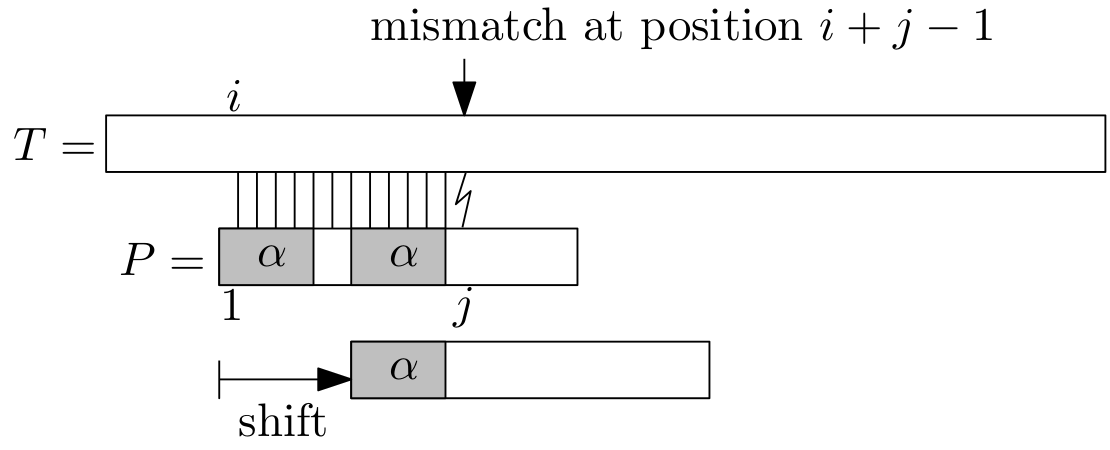
\includegraphics[width=0.7\textwidth]{KMP}
  \caption{Idee beim Verschieben des Patterns: \( \alpha \) wurde bereits gematcht. Früher als mit dem bereits gematchten Suffix kann das nächste Vorkommen von \( P \) nicht auftauchen, also kann mann \( P \) direkt um \( j - 1 - \alpha \) verschieben}
\end{figure}

Der Algorithmus besteht aus zwei Teilen:
\begin{enumerate}
  \item \textbf{Border-Array berechnen} (\( O(m) \)). Damit die oben erläuterten Verschiebungen nachher effizient durchgeführt werden können, berechnen wir für das leere Wort \emph{und} jeden Buchstaben in \( P \) einen \( \alpha \)-Wert. Diese Werte ergeben das \term{Border-Array}\label{def:borderArray}\index{Border-Array}:
  \begin{minipage}{.55\textwidth}
    \begin{equation*}
      \text{border}[j] = \begin{cases}
        -1\text{,} &\text{falls } j = 1 \\
        \alpha(P_{1 \dots j-1})\text{,} &\text{sonst}
      \end{cases}\text{.}
    \end{equation*}
  \end{minipage}
  \hfill
  \begin{minipage}{.35\textwidth}
    \begin{figure}[H]
      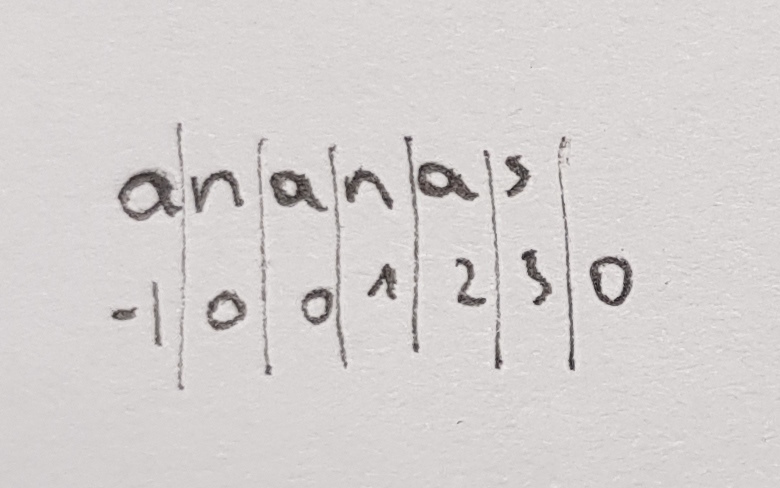
\includegraphics[width=.8\textwidth]{borderArray}
      \caption{Beispiel für das Border-Array eines Patterns}
    \end{figure}
  \end{minipage}

  \item \textbf{Pattern matchen} (\( O(n) \)). Nun verwenden wir das erstellte Border-Array, um Vorkommnisse von \( P \) in \( T \) zu finden. Wir starten sowohl im Text als auch im Pattern an Position 1 und fangen an zu matchen. Kommt es an Position \( 1 \leq j \leq m \) des Patterns zu einem Mismatch, so können wir \( P \) direkt um \( j - \text{border}[j] - 1 \) verschieben. In Pseudocode sieht das so aus:
  \begin{pseudocode}
    \textbf{\textsc{KMPMatch}} (P,T) \\
    \( i,j \coloneqq 1 \) \\
    \textbf{while} \( i \leq n - m + 1 \) \\
    \phantom{\quad} \textbf{while} \( j \leq m \wedge t_{i+j-1} = p_j \) \textbf{do} \( j \)++ \\
    \phantom{\quad} \textbf{if} \( j > m \) \textbf{then return} ``\( P \) occurs at pos \( i \) in \( T \) '' \\
    \phantom{\quad} \( i \) += \( j - \text{border}[j] + 1 \) \\
    \phantom{\quad} \( j \coloneqq \max\left \{ 1, \text{border}[j]+1 \right \} \)
  \end{pseudocode}
\end{enumerate}

Eine Ausführung des Algorithmus kann also folgendermaßen aussehen:
\begin{figure}[H]
  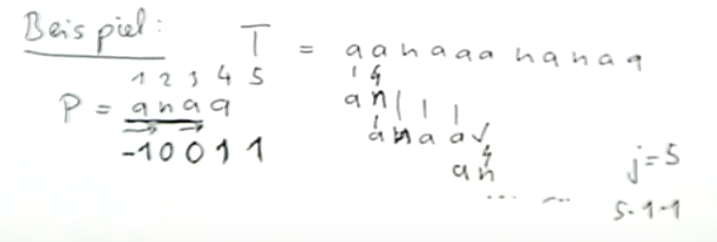
\includegraphics[width=.6\textwidth]{kmpBeispiel}
  \caption{Beispiel für das Verwenden des Knuth-Morris-Pratt-Algorithmus}
\end{figure}

\subsection{Suffix-Arrays}

Im Folgenden werden Arrays wieder mit Position \( 0 \) beginnen. Wir verwenden desweiteren folgende Festlegungen:
\begin{itemize}
  \item Ein \term{String}\index{String} ist ein Array von Buchstaben,
  \begin{equation*}
    S[0\dots n) \coloneqq S[0\dots n-1] \coloneqq [S[0],\dots,S[n-1]]\text{.}
  \end{equation*}
  \item Das \term{Suffix}\index{Suffix} \( S_i \) sei der Substring \( S[i\dots n) \) von \( S \).
  \item Wir setzen an das Ende jedes Strings ausreichend viele \term{Endmarkierungen}\index{Endmarkierung}: \( S[n] \coloneqq S[n+1] \coloneqq \cdots \coloneqq 0 \). \( 0 \) sei per Definition kleiner als alle anderen vorkommenden Zeichen.
\end{itemize}

Das \term{Suffix-Array}\index{Suffix-Array} eines Strings lässt sich nun folgendermaßen konstruieren:

\begin{minipage}{.65\textwidth}
  \begin{enumerate}
    \item Bilde die Menge aller Suffixe \( S_i \) (\( i = 0,\dots,n-1 \)) des Strings.
    \item Sortiere die Menge aller Suffixe des Strings (z.B. mit \hyperref[def:multikeyQuicksort]{Multikey Quicksort}).
  \end{enumerate}
\end{minipage}
\hfill
\begin{minipage}{.35\textwidth}
  \begin{figure}[H]
    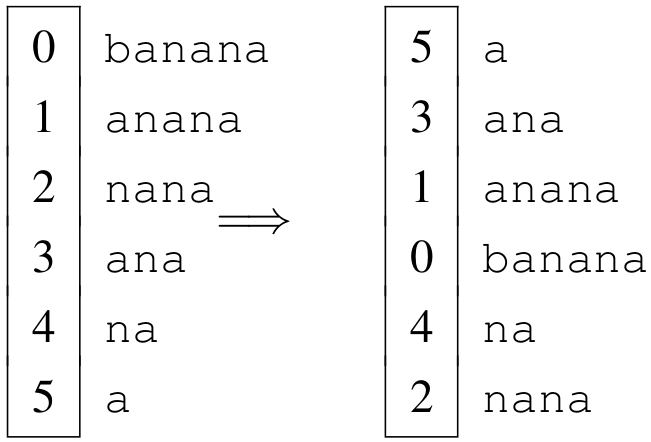
\includegraphics[width=.8\textwidth]{suffixArray}
    \caption{Beispiel für die Konstruktion des Suffix-Arrays des Strings ``\emph{banana}''}
  \end{figure}
\end{minipage}

Mithilfe dieses Suffix-Arrays lassen sich später viele Suchprobleme in Linearzeit lösen. Beispielsweise ist die Suche nach dem längsten Substring, der (eventuell mit Überschneidung) zweimal im Text vorkommt, linear --- dafür muss nach Berechnung des Suffix-Arrays der längste String gefunden werden, der Präfix von zwei Strings im Suffix-Array ist (im Beispiel oben wäre das ``\emph{ana}'').

\subsection{Suffix-Bäume}

Noch anschaulicher, allerdings wesentlich platzverbrauchender, sind \term{Suffix-Bäume}\index{Suffix-Baum} von Strings. Sie sind formal der \emph{kompaktierte Trie der Suffixe} und lassen sich (wenn auch sehr kompliziert) in \( O(n) \) berechnen.

\begin{minipage}{.65\textwidth}
  Bevor wir den Suffix-Baum eines Strings bilden hängen wir hinten an den String noch einen Charakter dran, der nicht im Alphabet des Strings vorkommt. Das hat den Vorteil, dass anschließend alle Suffixe in einem Blatt des Baums enden.
\end{minipage}
\hfill
\begin{minipage}{.35\textwidth}
  \begin{figure}[H]
    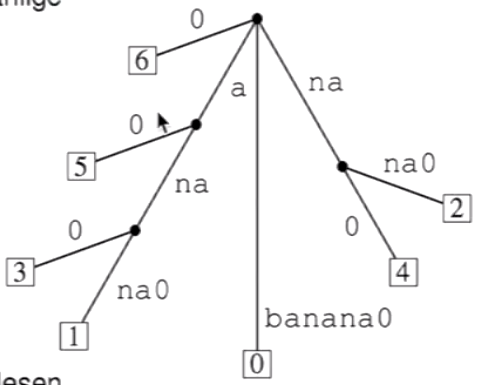
\includegraphics[width=.8\textwidth]{suffixTree}
    \caption{Beispiel für den Suffix-Baum des Strings ``\emph{banana}''}
  \end{figure}
\end{minipage}
  \chapter{Range Minimum Queries}

Eine \term{range minimum Query}\index{range minimum query} gibt für ein array \( A \) (\( \left\vert A \right\vert \eqqcolon n \)) die Position des kleinsten Elements zwischen zwei Begrenzern \( 1 \leq \bm{l} < \bm{r} \leq n \) zurück:
\begin{equation*}
  \text{rmq}_A(l,r) = (\text{arg})\min_{l \leq k \leq r}A[k]
\end{equation*}

\begin{figure}[H]
  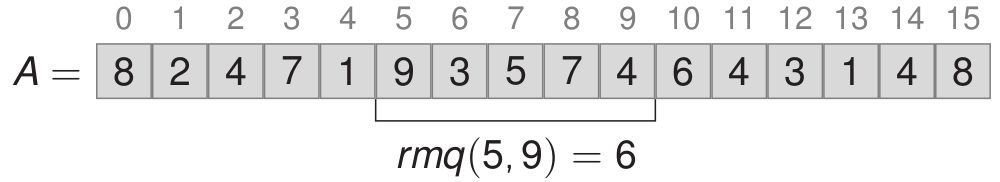
\includegraphics[width=0.6\textwidth]{rmqExample}
  \caption{Beispiel einer range minimum query}
\end{figure}

Ein naiver Ansatz, um eine range minimum query auszuführen, ist, einfach das Array zu durchlaufen und das Minimum zu speichern (und wenn nötig zu aktualisieren). Dafür ist keine Vorbereitungsarbeit nötig (also \( O(1) \)) und die Abfrage ist in \( O(n) \). Wir notieren
\begin{equation*}
  \left\langle O(1), O(n) \right\rangle\text{.}
\end{equation*}

\subsection{Lösung 1 --- \( \left\langle O(n), O(\log n) \right\rangle \)}

Baut man einen binären Suchbaum über das Array auf, so lässt sich die Komplexität der Abfrage auf \( O(\log n) \) reduzieren.

Hierzu betrachtet man die größtmöglichen Knoten, die vollständig im Abfrageintervall liegen (grün dargestellt), und berechnet das Minimum dieser.

\begin{figure}[H]
  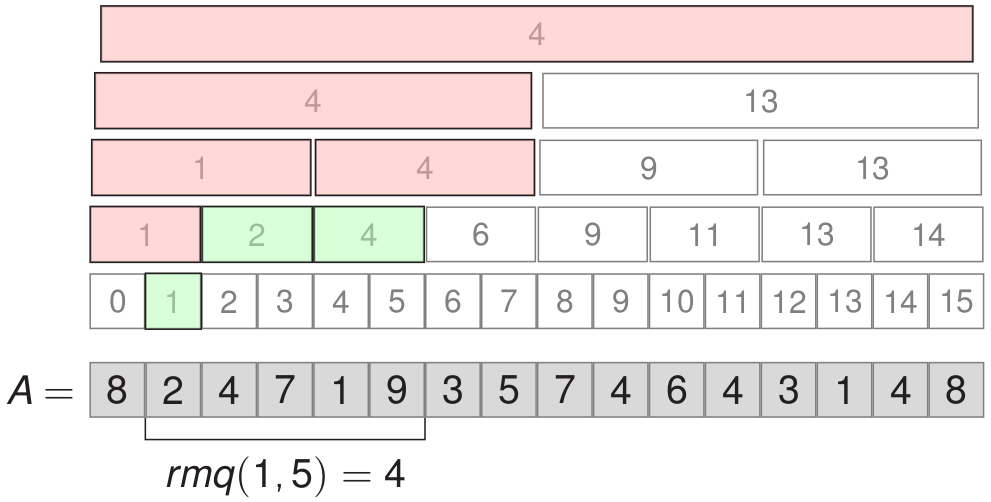
\includegraphics[width=0.6\textwidth]{rmqBST}
  \caption{Die grauen Felder stellen die Knoten des binären Suchbaums dar, sie beinhalten die Position des Arrays, an der der Teilbaum, dessen Wurzel sie sind, den minimalen Wert annimmt. Die größten Knoten, die vollständig im Intervall liegen, sind grün markiert.}
\end{figure}

\subsection{Lösung 2 --- \( \left\langle O(n\log n),O(1) \right\rangle \)}

Wir reduzieren nun die Zeit, die zum Bearbeiten der rmq benötigt wird, auf \( O(1) \), indem wir für jedes \( A[i] \) ein Array \( M_i[0,\log n] \) vorberechnen. Es sei
\begin{equation*}
  M_i[j] = \text{rmq}_A(i,i+2^j-1)\text{.}
\end{equation*}

Idee ist es nun, \( \text{rmq}_A(l,r) \) aus der Überdeckung des Intervalls durch zwei Zweierpotenzen zu berechnen.

Wir suchen dafür \( 2^{\lfloor l - r \rfloor} \), also die größte Zweierpotenz, die kleiner ist als die Länge des Intervalls. Offensichtlich ist diese Zweierpotenz mehr als halb so groß wie das Intervall, also ist \( \text{rmq}_A(l,r) \) entweder das Minimum der ersten oder zweiten überdeckenden Zweierpotenz.

\begin{figure}[H]
  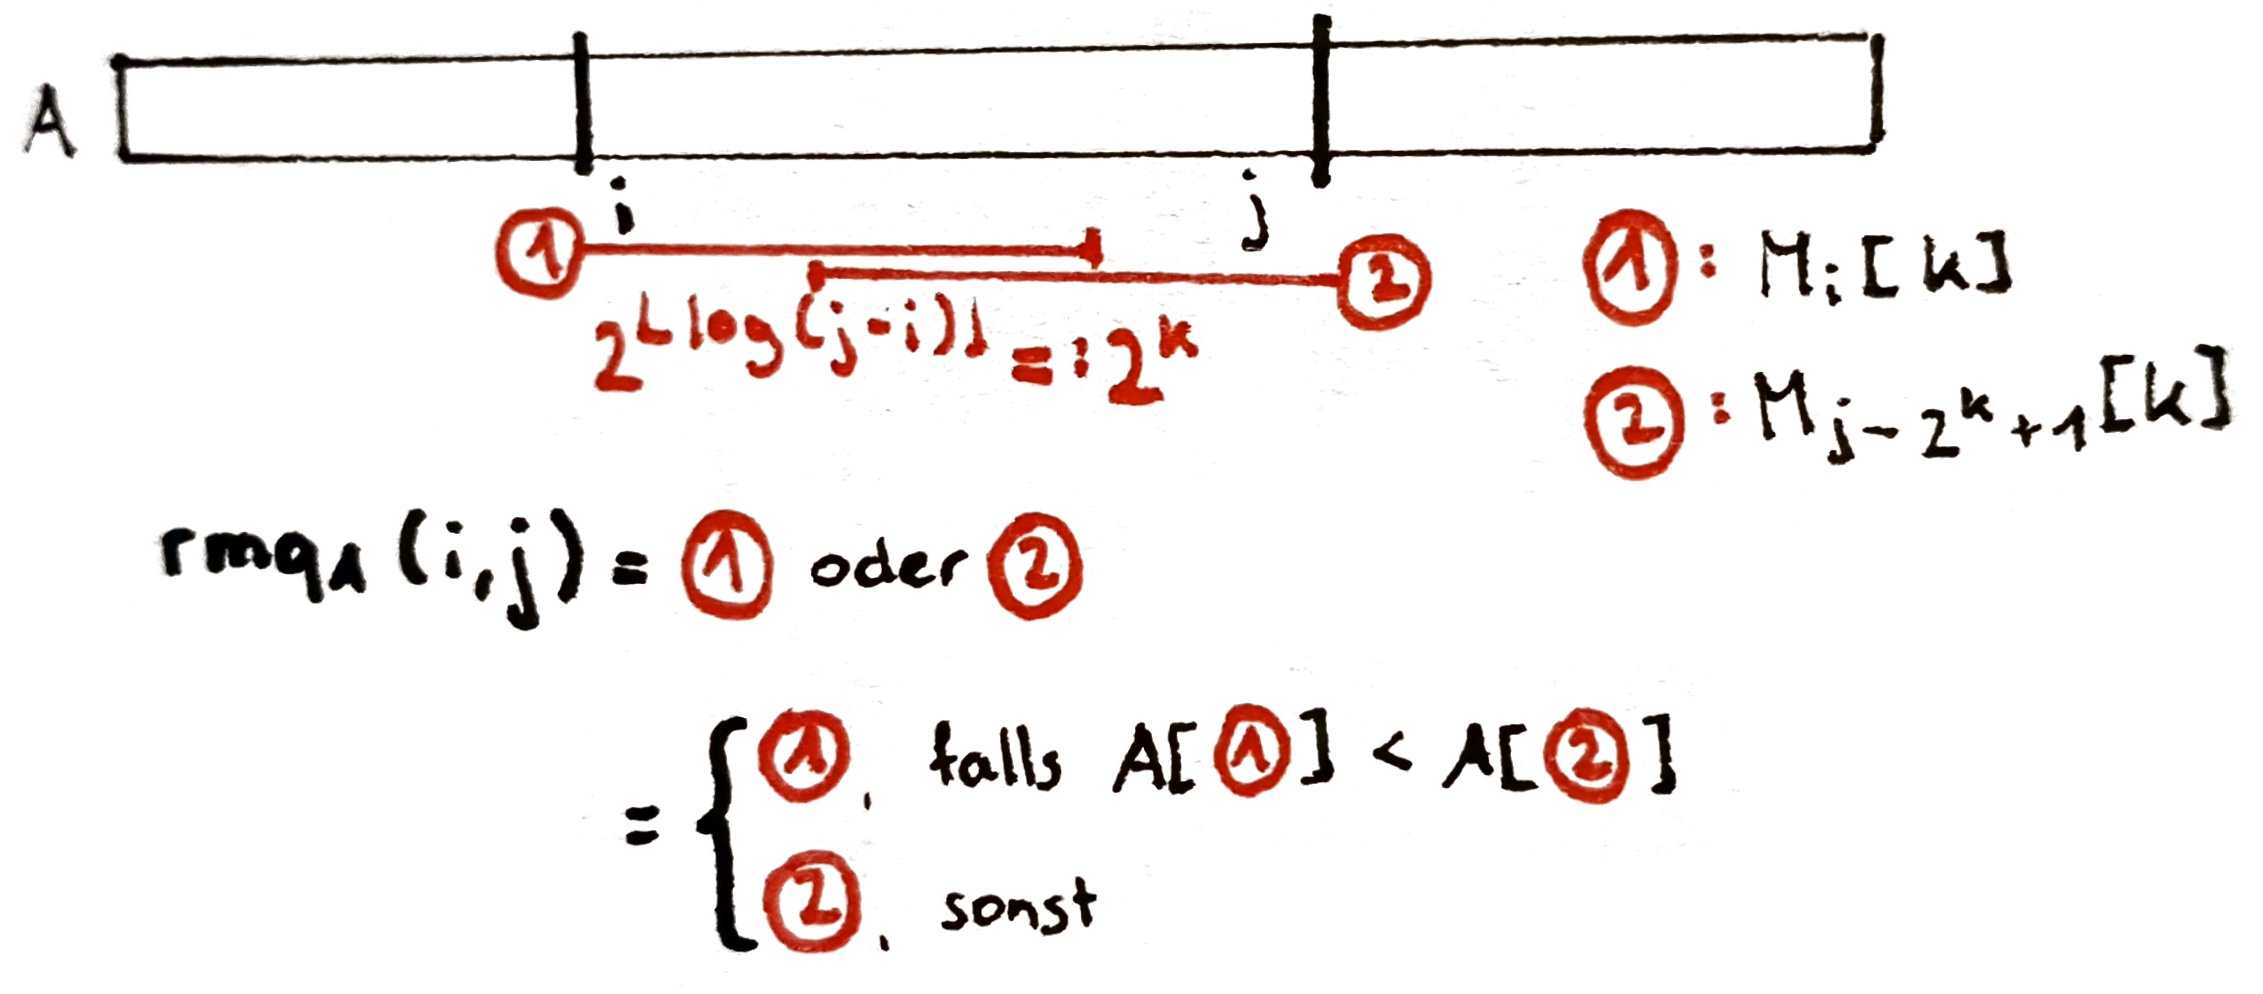
\includegraphics[width=0.6\textwidth]{rmqVersion2}
  \caption{Funktionsweise des zweiten rmq-Algorithmus}
\end{figure}

\subsection{Lösung 3 --- \( \left\langle O(n \log \log n), O(1) \right\rangle \)}

Wir wenden folgende Prozedur an:

\begin{enumerate}
  \item \( A \) in \( t = \frac{n}{\log n} \) Blöcke \( B_0, \dots, B_{t-1} \) der Größe \( \log n \) unterteilen.
  \item Array \( S[0,t-1] \) mit \( S[i] = \min\left \{ x \in B_i \right \} \) erstellen, rmq-Struktur nach Lösung 2 für \( S \) berechnen.
  \item Für jeden Block \( B_i \) rmq-Struktur nach Lösung 2 berechnen.
\end{enumerate}

Diese Prozedur liegt in \( O(n \log \log n) \).

Soll nun \( \text{rmq}_A(l,r) \) bestimmt werden, so geht das folgendermaßen:

\begin{enumerate}
  \item Bestimme die Blöcke \( l \in B_{l'} \) und \( r \in B_{r'} \).
  \item Berechne \( m = \text{rmq}_S(l'+1, r'-1) \). Wir nutzen also die Struktur über \( S \), um die rmq-Werte der Blöcke zwischen den beiden Grenzblöcken zu berechnen.
  \item Es seien \( k_0,k_1,k_2 \) die \( \text{rmq}_A \)-Resultate in den Blöcken \( l' \), \( r' \) und \( m \)
  \item \( \text{rmq}_A(l,r) = \text{arg}\min \left \{ A[k_0],A[k_1],A[k_2] \right \} \)\text{.}
\end{enumerate}
  \chapter{Burrows-Wheeler-Transformation}

Die \term{Burrows-Wheeler-Transformation}\index{Burrows-Wheeler-Transformation} erzeugt eine sinnvolle Permutation des eingegebenen Strings; sie gruppiert Zeichen mit ähnlichem Kontext nahe beieinander. Die Struktur der Permutation beinhaltet alle Informationen, die benötigt werden, um eine Rücktransformation durchzuführen, es sind also keine Zusatzinformationen nötig. Hin- und Rücktransformation geht in \( O(n) \). Sie wird hauptsächlich zur Vorverarbeitung statischer Texte genutzt, um sie komprimieren, indizieren und in ihnen suchen zu können.

\section{Konstruktion}

Sei \( T = \texttt{lalalangng\$} \) der gegebene String (mit angehängtem \$-Zeichen), \( n = \left\vert T \right\vert \) und \( T^{(i)} \) die \( i \)-te Permutation von \( T \) (durch \( i \) mal den vordersten Buchstaben nehmen und hinten anhängen). Man erhält die Burrows-Wheeler-Transformation von \( T \) so:

\begin{enumerate}
  \item Schreibe \( T^{(1)} \) bis \( T^{(n)} \) untereinander.
  \item Sortiere \( T^{(1)} \) bis \( T^{(n)} \).
  \item Die letzte Spalte ist \( T^{\text{BWT}} \) (\( = L \)), die Burrows-Wheeler-Transformation von \( T \).
\end{enumerate}

\begin{figure}[H]
  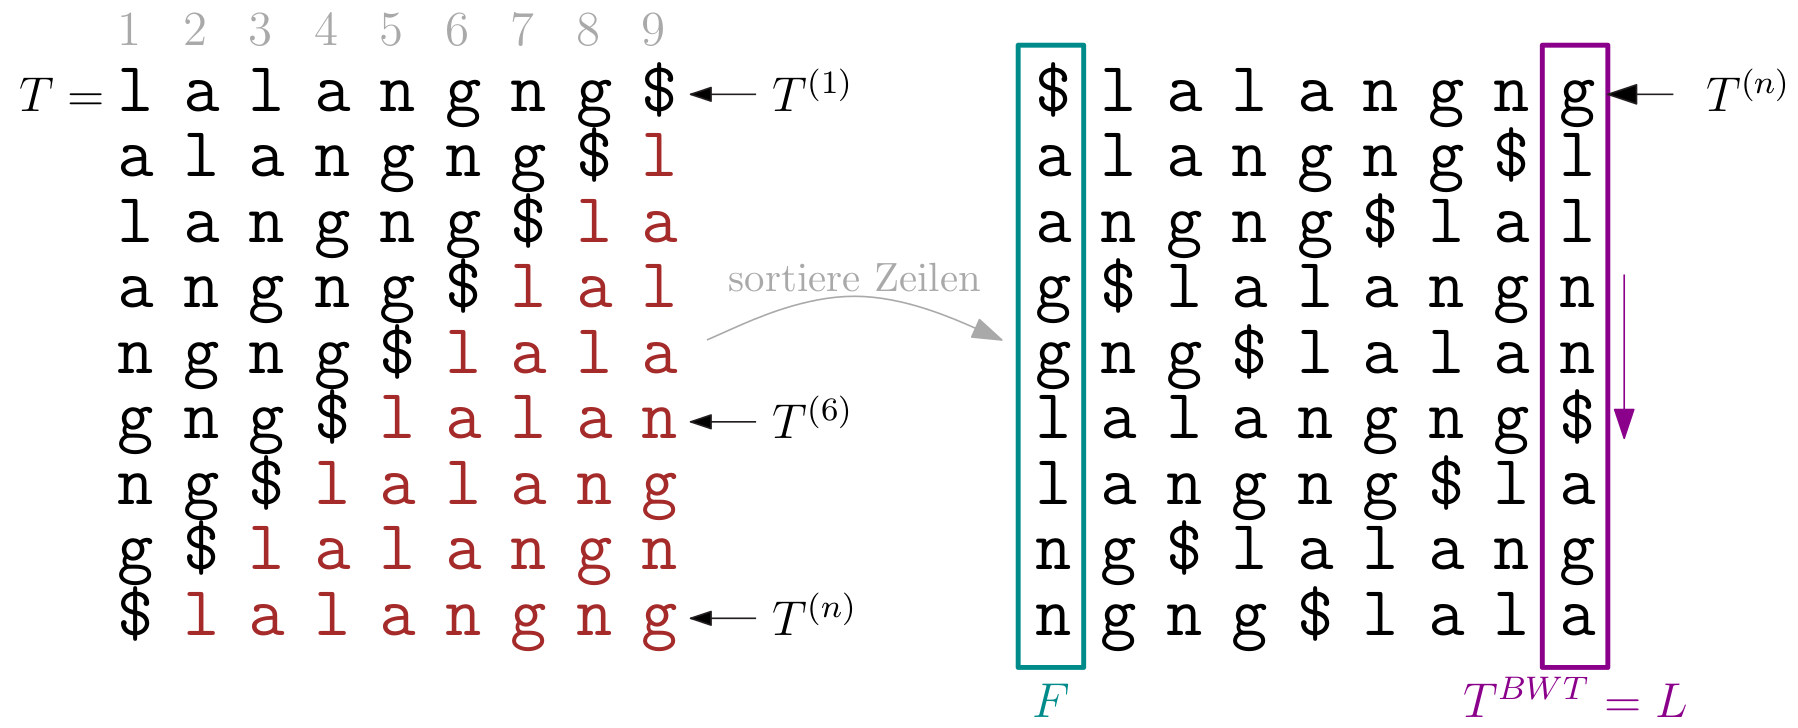
\includegraphics[width=0.7\textwidth]{BWT}
  \captionsetup{width=.7\textwidth}
  \caption{Konstruktion der Burrows-Wheler-Transformation von \( T = \texttt{lalalangng\$}  \), \( T^{\text{BWT}} = \texttt{gllnn\$ aga} \). Da \( T^{\text{BWT}} \) die letzte Spalte ist schreibt man oft auch \( L \) stattdessen. Die erste Spalte wird auch \( F \) genannt}
\end{figure}

Naiv benötigt die Berechnung von \( T^{\text{BWT}} \) \( O(n^2 + n\log n) \) Schritte. Die Berechnungszeit lässt sich aber auf \( O(n) \) reduzieren.

\section{Beobachtungen}

Folgende Eigenschaften lassen sich feststellen:

\begin{itemize}
  \item Die Zeilen der oben konstruierten Matrix enthalten die sortierten Suffixe von \( T \) (vom Zeilenstart bis \$ gehend).
  \item Die Zeichen der letzten Spalte (also \( T^{\text{BWT}} \)) sind also die Zeichen, die vor dem zu ihrer Zeile gehörenden Suffix stehen. Formaler ist \( T^{\text{BWT}}[i] \) das Zeichen vor dem \( i \)-ten Suffix in \( T \):
  \begin{equation*}
    T^{\text{BWT}}[i] = L[i] = T[\text{SA}[i]-1] = T^{(\text{SA}[i])}[n]
  \end{equation*}
  Da wir mithilfe des \hyperref[sec:SALinear]{DC3-Algorithmus} das Suffix-Array in Linearzeit berechnen können, können wir auch die Burrows-Wheeler-Transformation in Linearzeit bestimmen.
\end{itemize}

\section{Rücktransformation}

\begin{minipage}{0.8\textwidth}
  Wir können aus einer vorliegenden \( T^{\text{BWT}} \) einfach \( F \) --- also die erste Spalte der Matrix --- konstruieren, indem wir die Buchstaben von \( T^{\text{BWT}} \) sortieren. Hängen wir nun \( T^{\text{BWT}} \) und \( F \) hintereinander, so haben wir bereits Buchstabenpaare, die so auch in \( T \) auftreten. Sortieren wir nun die beiden Spalten (also die Buchstabenpaare) lexikographisch, so erhalten wir die auf \( F \) folgende Spalte. Durch diesen Prozess lässt sich die gesamte Matrix und somit \( T \) rekonstruieren.
\end{minipage}
\hfill
\begin{minipage}{0.15\textwidth}
  \begin{figure}[H]
    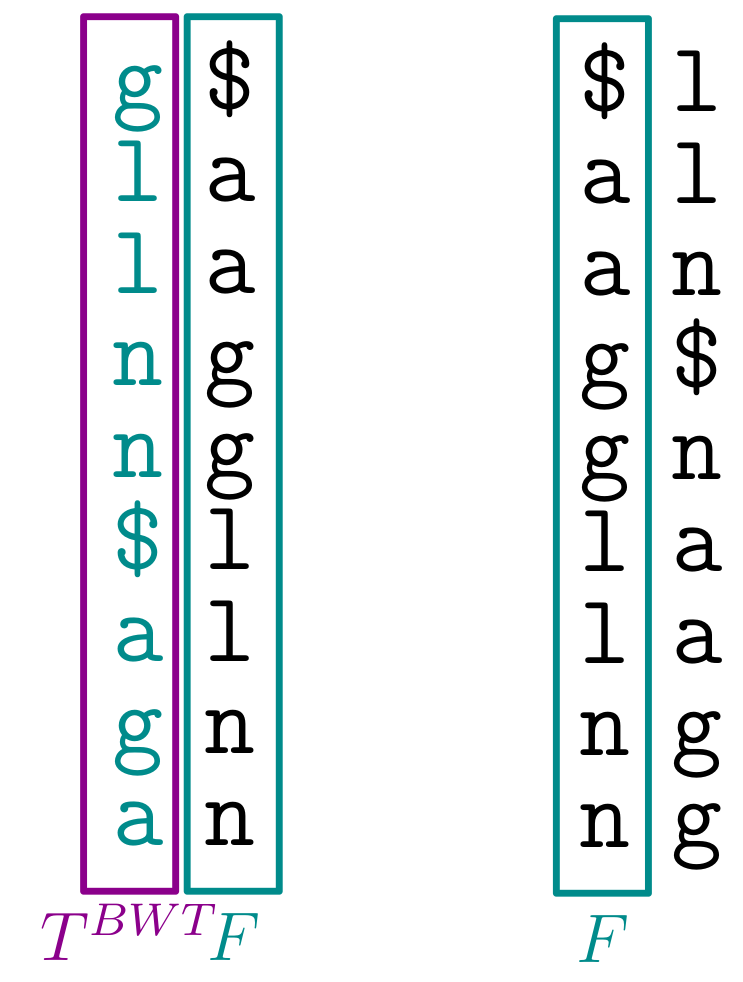
\includegraphics[width=\textwidth]{BWTSorting}
  \end{figure}
\end{minipage}

Diese Art der Rücktransformation benötigt \( O(n^2\log n) \) Schritte. Im Folgenden werden wir die Rücktransformation auf Linearzeit reduzieren. Dazu benötigen wir \term{Last-to-front mapping}\index{Last-to-front mapping}:
\begin{equation*}
  \text{LF}[i] \coloneqq \text{ Position in } L\text{, an der Vorgänger von } L[i] \text{ steht}
\end{equation*}

\begin{minipage}{.65\textwidth}
  Da die Spalten der BWT-Matrix zyklisch sind, ist der Vorgänger von \( L[i] \) derjenige Buchstabe, der in \( F[i] \) steht, also
  \begin{equation*}
    \text{LF}[i] = \text{Position, an der } L[i] \text{ in } F \text{ steht}
  \end{equation*}
\end{minipage}
\hfill
\begin{minipage}{.3\textwidth}
  \begin{figure}[H]
    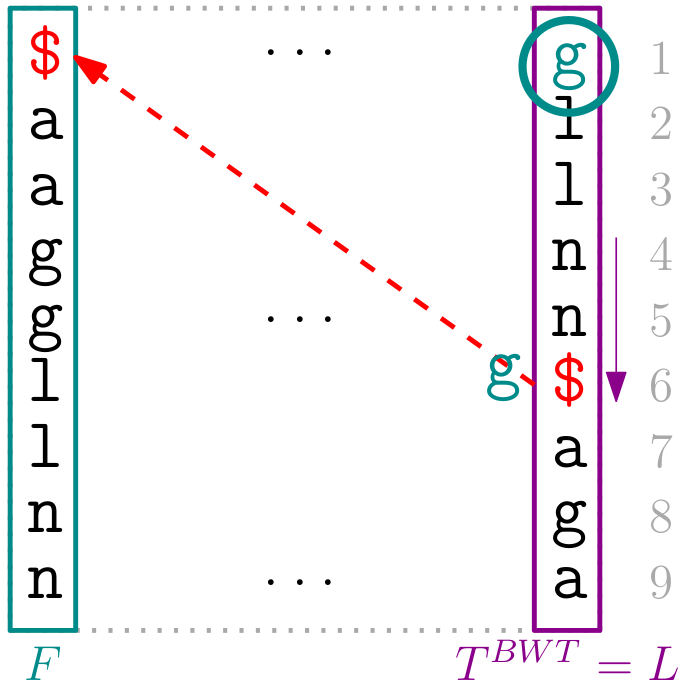
\includegraphics[width=\textwidth]{BWTLF}
    \caption{Gesucht ist der Vorgänger von \texttt{\$}. Stellen wir uns \( T^{\text{BWT}} \) ein zweites Mal links von \( F \) vor, so sehen wir, dass es \texttt{g} ist}
  \end{figure}
\end{minipage}

Wir erhalten folgenden Zusammenhang:
\begin{equation*}
  \text{LF}[i] = j \Leftrightarrow T^{(\text{SA}[j])} = {\left( T^{(\text{SA}[i])} \right)}^{(n)}\text{.}
\end{equation*}

\subsection{Weitere Überlegungen zur Rücktransformation}

Wir können desweiteren folgende Beobachtungen an \( T^{\text{BWT}} \) machen:

\begin{minipage}{.6\textwidth}
  \begin{itemize}
    \item Gleiche Zeichen haben gleiche Reihenfolge in \( F \) und \( L \).
    \item Falls \( L[i] = L[j] \) für \( i < j \), dann ist \( \text{LF}[i] < \text{LF}[j] \).
  \end{itemize}
  Grund dafür ist, dass die Zeilen der BWT-Matrix lexikographisch sortiert sind.
\end{minipage}
\hfill
\begin{minipage}{.35\textwidth}
  \begin{figure}[H]
    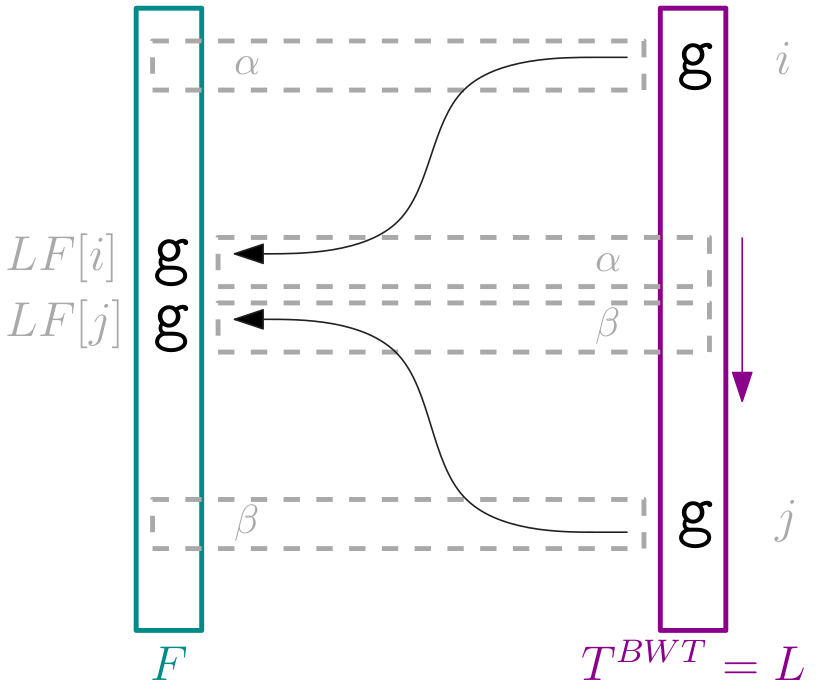
\includegraphics[width=\textwidth]{BWTBack}
    \caption{Präfixe \( \alpha \) und \( \beta \) und wie sie in der Matrix vorkommen}
  \end{figure}
\end{minipage} \\

Wir können also \( LF \) rein aus \( T^{\text{BWT}} \) berechnen. Dazu brauchen wir nur zwei Hilfsfunktionen:

\begin{itemize}
  \item \( C(a) \coloneqq \# \) Zeichen \( < a \)
  \item \( \text{occ}[i] \coloneqq \# \) Zeichen \( = L[i] \) in \( L[1\dots i] \)
\end{itemize}

Nun können wir \( \text{LF}[i] \) darstellen als
\begin{equation*}
  \text{LF}[i] = C(L[i]) + \text{occ}[i]
\end{equation*}
und können somit \( \text{LF} \) in \( O(n) \) berechnen, da sich \( C \) und \( \text{occ} \) in Linearzeit berechnen lassen.

\subsection{Implementierung}

Zuerst berechnen wir LF. Hier sieht die Implementierung so aus:

\begin{enumerate}
  \item Initialisiere occ und \( h \). \( h \) sei ein Array, das zählt, wie oft ein bestimmter Buchstabe vorkommt, damit wir nachher \( C \) gescheit berechnen können.
  \item Laufe durch \( L = T^{\text{BWT}} \) (\( i = 1 \dots n \))
  \begin{itemize}
    \item \( h(L[i]) \)++
    \item \( \text{occ}(L[i]) = h(L[i]) \)
  \end{itemize}
  \item Konstruiere \( C \) aus \( h \): \( C(\texttt{\$}) = 0 \), \( C(\alpha) = C(\alpha - 1) + h(\alpha - 1) \) (\( \alpha \) ist ein Buchstabe, \( \alpha - 1 \) sein Vorgänger)
  \item \( \text{LF}[i] = C(L[i]) + \text{occ}[i] \)
\end{enumerate}

\begin{figure}[H]
  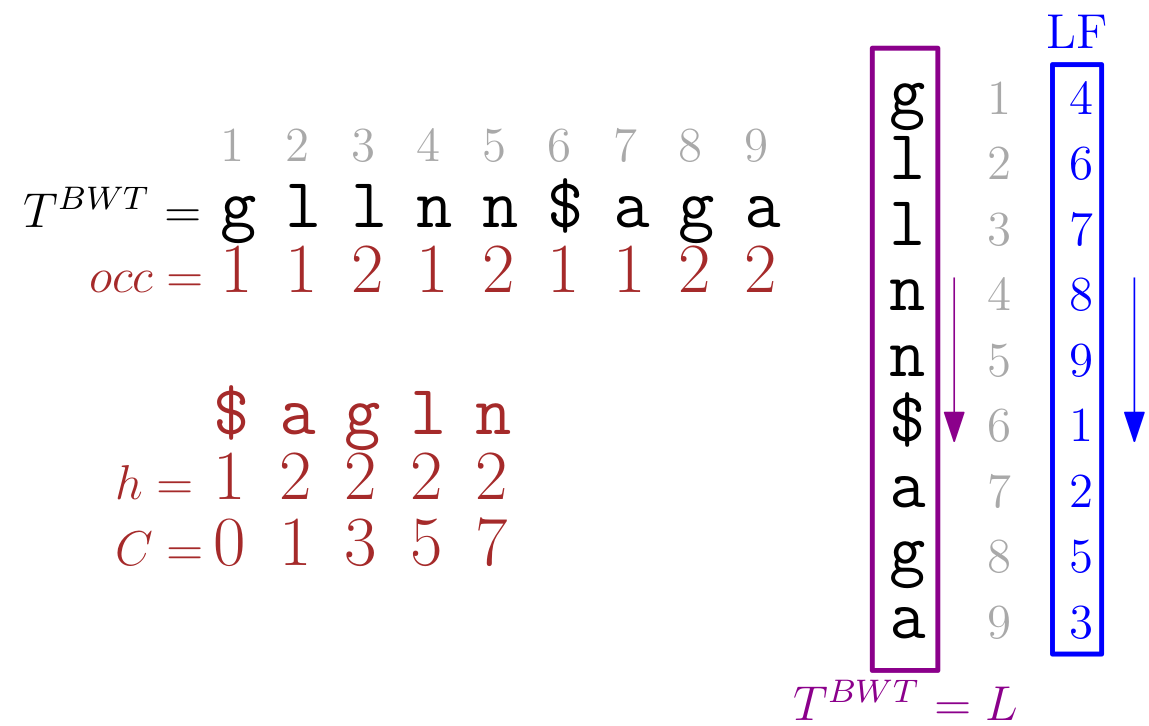
\includegraphics[width=0.5\textwidth]{BWTBackLinear}
  \caption{Beispiel des Algorithmus zur Berechnung von LF nach Durchführung}
\end{figure}

\begin{minipage}{.8\textwidth}
  Nun kann \( T \) von rechts nach links berechnet werden:
  \begin{enumerate}
    \item \( T[n] = \texttt{\$} \Rightarrow \text{LF}[\cdot] = 1 \). Das ist unabhängig von \( T \) so.
    \item \( L[1] = \texttt{g} \Rightarrow T[n-1] = \texttt{g} \Rightarrow \text{LF}[1] = 4 \)
    \item \( L[4] = \texttt{n} \Rightarrow T[n-2] = \texttt{n} \Rightarrow \cdots \)
  \end{enumerate}
  Also geht auch die Rücktransformation in \( O(n) \).
\end{minipage}
\hfill
\begin{minipage}{.15\textwidth}
  \begin{figure}[H]
    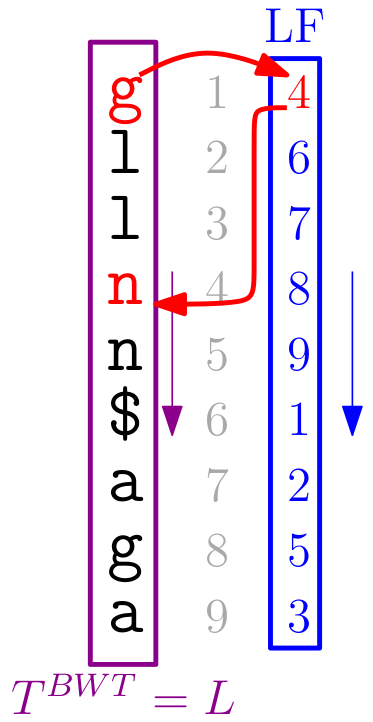
\includegraphics[width=\textwidth]{BWTBackResult}
  \end{figure}
\end{minipage}

\section{Was bringt die BWT?}

Die Vorteile der Burrows-Wheeler-Transformation sind nicht direkt erkennbar --- sie nutzt dieselben Zeichen wie \( T \) und benötigt den gleichen Platz.

Allerdings wird die \emph{Komprimierung stark vereinfacht}, weil Zeichen mit ähnlichem Kontext gruppiert werden. Besonders gut funktioniert sie auf Texten mit vielen gleichen Substrings, wie beispielsweise einem englischen Fließtext. Zur Vereinfachung von \emph{Indexierung} und \emph{Suche} steuert sie auch bei, weil Vorgänger von Suffixen einfach bestimmt werden können.

Im Folgenden werden wir uns die Burrows-Wheeler-Transformation im Kontext von \emph{Kompression} und \emph{Suche} anschauen.

\section{Kompression}

Wir schauen uns zwei Kompressionsmöglichkeiten an: die \emph{move to front}-Kodierung und die Huffman-Kodierung

\subsection{MTF-Kodierung}

Idee der \term{MTF-Kodierung}\index{Kodierung!MTF} ist es, lokale Redundanz zu nutzen und so kleine Zahlen für gleiche Zeichen, die nahe beieinander liegen, zu verwenden. Die Umsetzung funktioniert so:

\begin{enumerate}
  \item Initialisiere \( Y \) mit Alphabet von \( T^{\text{BWT}} \).
  \item Durchlaufe \( T^{\text{BWT}} \) (\( i = 1,\dots,n \))
  \begin{itemize}
    \item Generiere \( R[1,\dots,n] \), wobei \( R[i] \) die Position von \( T^{\text{BWT}}[i] \) in \( Y \) codiert.
    \item Schiebe \( T^{\text{BWT}}[i] \) an den Anfang von \( Y \).
  \end{itemize}
\end{enumerate}

\begin{figure}[H]
  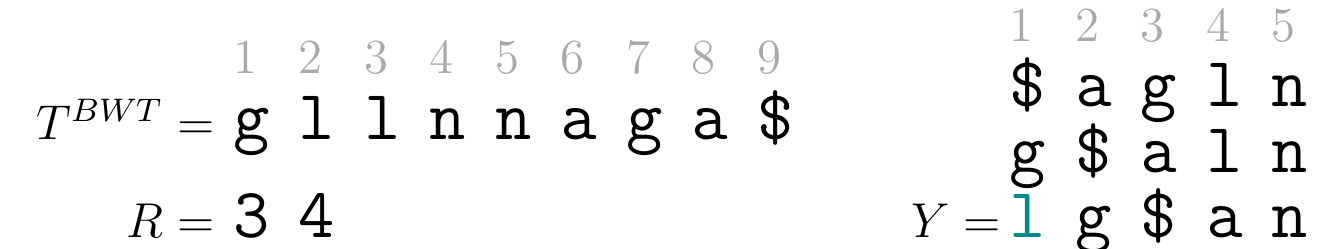
\includegraphics[width=0.8\textwidth]{MTF}
  \caption{Es wurde hier gerade die \texttt{4} eingefügt und deswegen \texttt{l} in \( Y \) nach vorne genommen. Als nächstes muss \texttt{l} codiert (\( \cong \texttt{1} \)) und \( Y \) anschließend nicht verändert werden, weil \texttt{l} ja eh schon ganz vorne steht}
\end{figure}

\subsection{Huffman-Kodierung}

Die \term{Huffman-Kodierung}\index{Kodierung!Huffman} erzeugt präfixfreie Codes variabler Länge. Der Ablauf ist:

\begin{enumerate}
  \item Notiere vorkommende Symbole und ihre jeweiligen Häufigkeiten. Sie sind die Blätter des (binären) Huffman-Baumes.
  \item Verknüpfe die zwei seltenstem Knoten in einem neuen Knoten. Die Häufigkeit des neuen Knotens ist die Summe der Häufigkeiten seiner Kinder. Dies erfolgt nun iterativ.
  \item Die Wurzel hat relative Häufigkeit \( 1 \) (bzw.\ absolute Häufigkeit \( \left\vert T \right\vert \)).
  \item Beschrifte die Kanten zwischen einem Knoten und seinen beiden Kindern mit \( 0 \) und \( 1 \). Der Pfad von der Wurzel zu einem bestimmten Blatt ergibt den Code des Symbols, zu dem das Blatt gehört.
\end{enumerate}

\begin{figure}[H]
  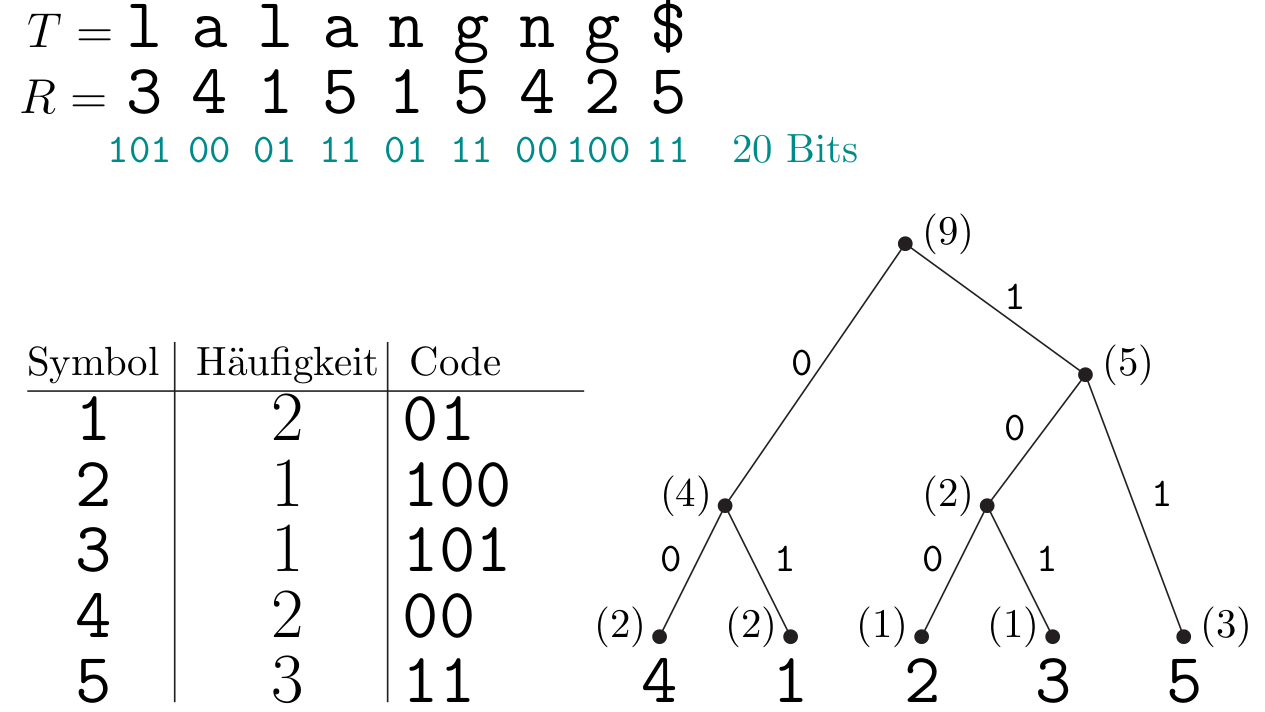
\includegraphics[width=0.5\textwidth]{Huffman}
  \captionsetup{width=.5\textwidth}
  \caption{MTF-Kodierung \( R \) von \( T \), die Häufigkeit der in \( R \) vorkommenden Symbole und die mit dem Huffman-Baum erzeugten Codes}
\end{figure}

\section{Suche in der Burrows-Wheeler-Transformation}

Wir möchten nun in \( T^{\text{BWT}} \) nach einem Pattern \( P \) suchen. Hier sei
\begin{align*}
  P &= \texttt{bar} \quad \text{und} \\
  T &= \texttt{abracadabrabarbara\$}\quad\text{und somit} \\
  \text{BWT} &= \texttt{arrd\$rcbbraaaaaabba}
\end{align*}
Wir benötigen dazu zwei Hilfsmittel:

\begin{itemize}
  \item Das Array \( C \) beinhalte für jeden eindeutigen Buchstaben in \( t \in T \) die Position des ersten Suffixes im Suffix-Array, das mit \( t \) beginnt.
  \item \( \text{rank}(i,X,\text{ BWT}) \) gibt an, wie oft ein Buchstabe \( X \) in \( \text{BWT}[0,\dots,i-1] \) vorkommt.
\end{itemize}

Wir suchen nun nach \( P \) in BWT. Wir suchen rückwärts, starten also mit ``\texttt{r}''. Dazu ermitteln wir alle Suffixe, die mit \texttt{r} starten. Wir nutzen dazu \( C \) und rank:

\begin{itemize}
  \item Initiales Intervall: \( [\text{sp}_0, \text{ep}_0] = [0,\dots,n-1] \).
  \item Ermittle Intervall der Suffixe, die mit \texttt{r} starten:
  \begin{itemize}
    \item \( \text{sp}_1 = C[r] + \text{rank}(\text{sp}_0, \texttt{r}, \text{BWT}) = 15 + \text{rank}(0,\texttt{r}, \text{BWT}) = 15+0 = 15 \)
    \item \( \text{ep}_1 = C[r] + \text{rank}(\text{ep}_0 + 1, \texttt{r}, \text{BWT}) - 1 = 15 + 4 - 1 = 18 \)
  \end{itemize}
\end{itemize}

\begin{minipage}{.7\textwidth}
  Wir suchen nun analog nach ``\texttt{ar}'', indem wir \( \text{sp}_2 \) und \( \text{ep}_2 \) aus \( \text{sp}_1 \) und \( \text{ep}_1 \) berechnen. Das Ganze dann nochmal für ``\texttt{bar}'' und wir erhalten 9 und 10 als diejenigen Suffixe, die mit \texttt{bar} anfangen.
\end{minipage}
\hfill
\begin{minipage}{.25\textwidth}
  \begin{figure}[H]
    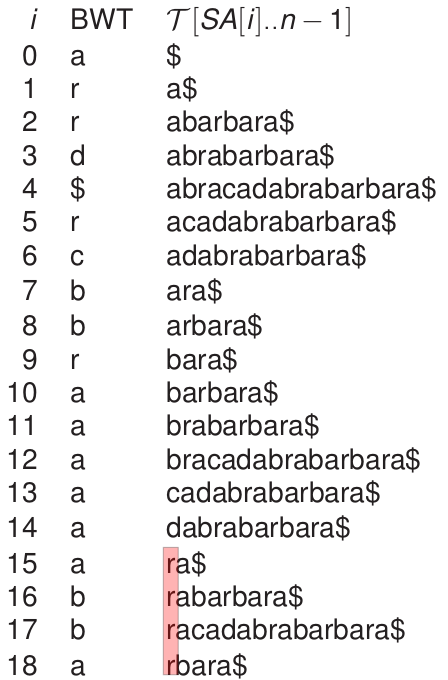
\includegraphics[width=\textwidth]{BWTSearch}
    \caption{Intervall \( [\text{sp}_1, \text{ep}_1] \)}
  \end{figure}
\end{minipage}

\subsection{Zusammenfassung}

Wir brauchen also nur \( C \) und \( R \), um Abfragen zu Existenz und Anzahl eines Patterns machen zu können. Die Ausführungszeit ist in \( O(m*t_{\text{rank}}) \), wobei \( t_{\text{rank}} \) die Ausführungszeit einer rank-Operation ist.

Als nächstes werden wir uns damit beschäftigen, wie wir die rank-Operation implementieren können. Wir werden dazu \emph{wavelet trees}\footnote{Grossi \& Vitter, 2003} verwenden.

\section{Wavelet Trees}

\term{Wavelet Trees}\index{Wavelet Tree} erlauben ein schnelles Berechnen der rank-Operation. Dazu wird in einem Baum codiert, ob ein bestimmter Buchstabe des Strings (hier des BWT) in der oberen oder der unteren Hälfte des Alphabets liegt. So werden die Buchstaben des BWT einem Kindknoten zugeordnet, wo auf dem jeweiligen Teilalphabet erneut eine Zweiteilung stattfindet. Dieser Prozess wiederholt sich so lange, bis in jedem Blatt nur Zeichen einer Art stehen.

\begin{figure}[H]
  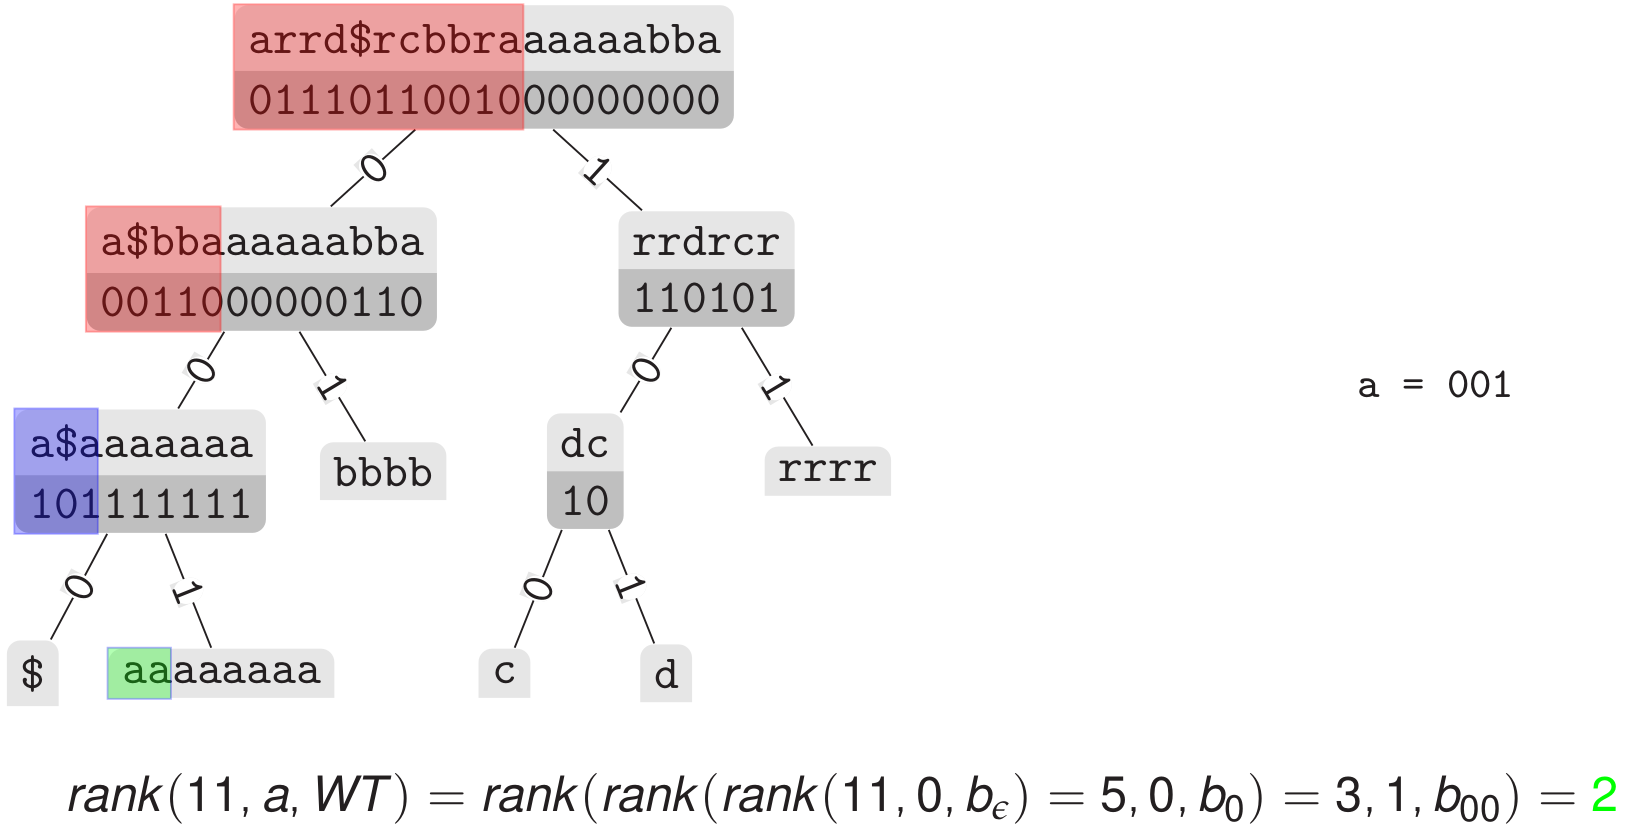
\includegraphics[width=0.8\textwidth]{WaveletTree}
  \caption{Wavelet Tree einer BWT und zugehörige Berechnung von \( \text{rank}(11, \textsc{a}, \text{BWT}) \)}
\end{figure}

Abfragen können auf einem Wavelet Tree in konstanter Zeit durchgeführt werden. Der Wavelet Tree selbst benötigt \( o(n) \) viel Platz, genauer
\begin{equation*}
  O\left( \frac{n}{\log n} + \frac{n \log \log n}{\log n} + \sqrt{n}\log n \log\log n \right)\text{.}
\end{equation*}

Die Konstruktion des Wavelet-Trees ist nicht zwingend an die Unterteilung des BWT zwei lexikographische Teilalphabete gebunden. Beispielsweise lässt sich eine Unterteilung in zwei Teilwörter auch durch die Häufigkeit der Buchstaben konstruieren, wodurch ein \term{Huffman-Wavelet-Tree}\index{Wavelet Tree!Huffman} entsteht.

\section{Exkurs --- Succinct Data Structures}

\textcolor{red}{\textbf{Hinweis}}: Dieser Abschnitt ist \emph{nicht} klausurrelevant!

\ \\

Eine extrem platzeffiziente Datenstruktur, \term{succinct data structure}\index{succinct data structure} genannt, benötigt nur wenig mehr Platz als die informationstheoretische untere Grenze, unterstützt allerdings Operationen zeiteffizient.

Sei \( L \) die informationstheoretische untere Schranke, die zur Repräsentierung einer Klasse von Objekten benötigt wird. Eine Datenstruktur, die Operationen trotzdem zeiteffizient unterstützt, heißt
\begin{itemize}
  \item \emph{implicit}, falls sie \( L + O(1) \) Bits Platz braucht (also nur konstant mehr als die informationstheoretische untere Schranke, z.B. Heap),
  \item \emph{succinct}, falls sie \( L + o(L) \) Bits Platz braucht (also nur sublinear mehr als die informationstheoretische untere Schranke, z.B. Baum),
  \item \emph{compact}, falls sie \( O(L) \) Bits Platz braucht. 
\end{itemize}

\subsection{Binärbäume --- succinct}

Es gibt \( C_n = \frac{1}{n+1}\binom{2n}{n} \) Binärbäume auf \( n \) Knoten. Um einen Binärbaum auf \( n \) Knoten speichern zu können, brauchen wir \( \log C_n = 2n + o(n) \) bits.\footnote{Das kann mithilfe der Sterling-Approximation gezeigt werden.} Wir wollen folgende Operationen unterstützen:
\begin{itemize}
  \item \( \text{parent}(v) \)
  \item \( \text{leftchild}(v) \)
  \item \( \text{rightchild}(v) \)
\end{itemize}

Eine mögliche Kodierung wäre, zu jedem Knoten des Baumes, der kein Blatt ist, so viele imaginäre Knoten hinzuzufügen, dass der jeweilige Knoten zwei Kinder hat (also entweder, 0, 1 oder 2 imaginäre Knoten). Diesen Prozess führt man durch, bis alle Blätter des Baumes dieselbe Tiefe haben. Wir können nun alle Knoten durchnummerieren und pro Knoten in einem Bit-Array speichern, ob der Knoten real (=1) ist oder nicht (=0).

\begin{figure}[H]
  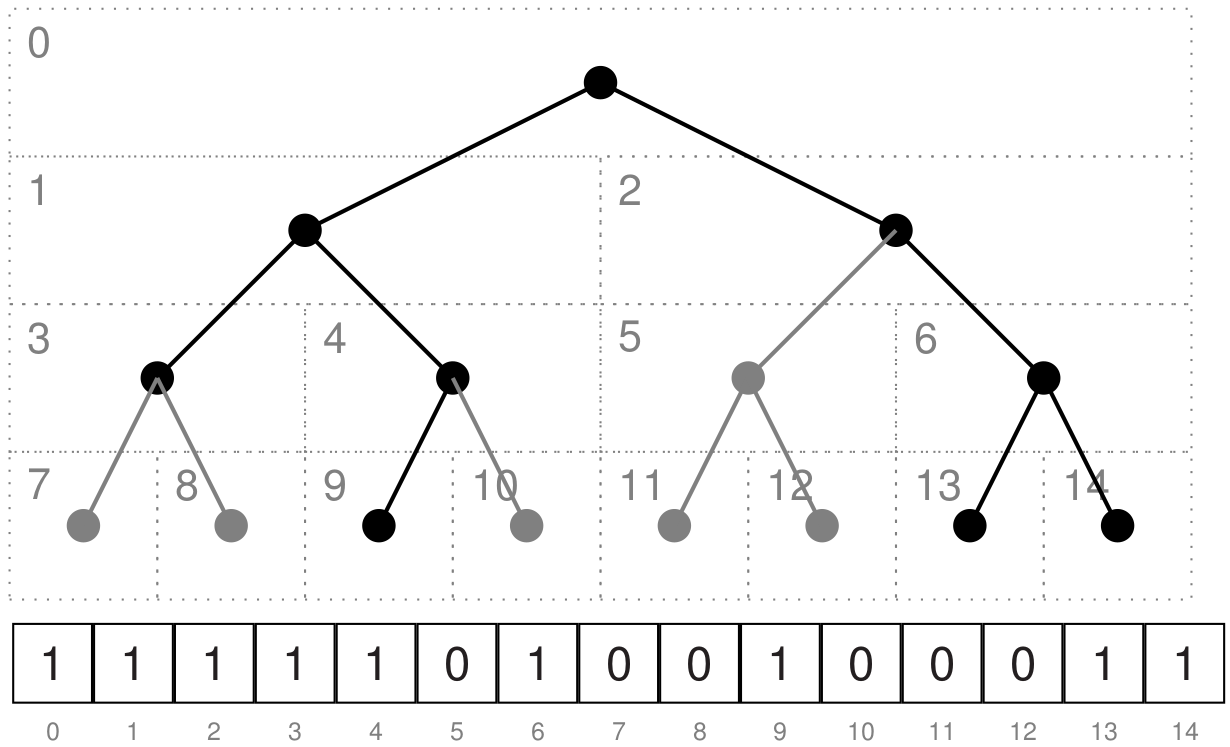
\includegraphics[width=0.5\textwidth]{SuccinctBinaryTree}
  \caption{Die schwarzen Knoten sind die realen Knoten des Baumes, die grauen die imaginären}
\end{figure}

Die geforderten Operationen können hier sehr einfach implementiert werden:
\begin{itemize}
  \item \( \text{parent}(v) = \left\lfloor \frac{v-1}{2} \right\rfloor \) (für \( v \neq \) Wurzel)
  \item \( \text{leftchild}(v) = 2v + 1 \)
  \item \( \text{rightchild}(v) = 2v + 2 \)
\end{itemize}

Problem dieses Ansatzes ist, dass für einen Binärbaum mit einer Maximaltiefe \( d \) stets \( 2^d \) Bits benötigt werden.

Jacobson schlug 1989 einen besseren Algorithmus vor:

\begin{enumerate}
  \item Alle Knoten des Binärbaums mit \( 1 \) markieren.
  \item Kinder jedes Knotens im Baum mit imaginären Knoten auf \( 2 \) ergänzen.
  \item Bit-Markierungen wie im vorhergehenden Algorithmus ablesen.
\end{enumerate}

Benötigt wird eine weitere Operation \( \text{rank}(i, \texttt{type}, b) \), die für Knoten \( i \) des ergänzten Baums \( b \) zurückgibt, um den wievielten Knoten des Typs \texttt{type} es sich handelt. Wir erhalten folgendes Resultat:

\begin{figure}[H]
  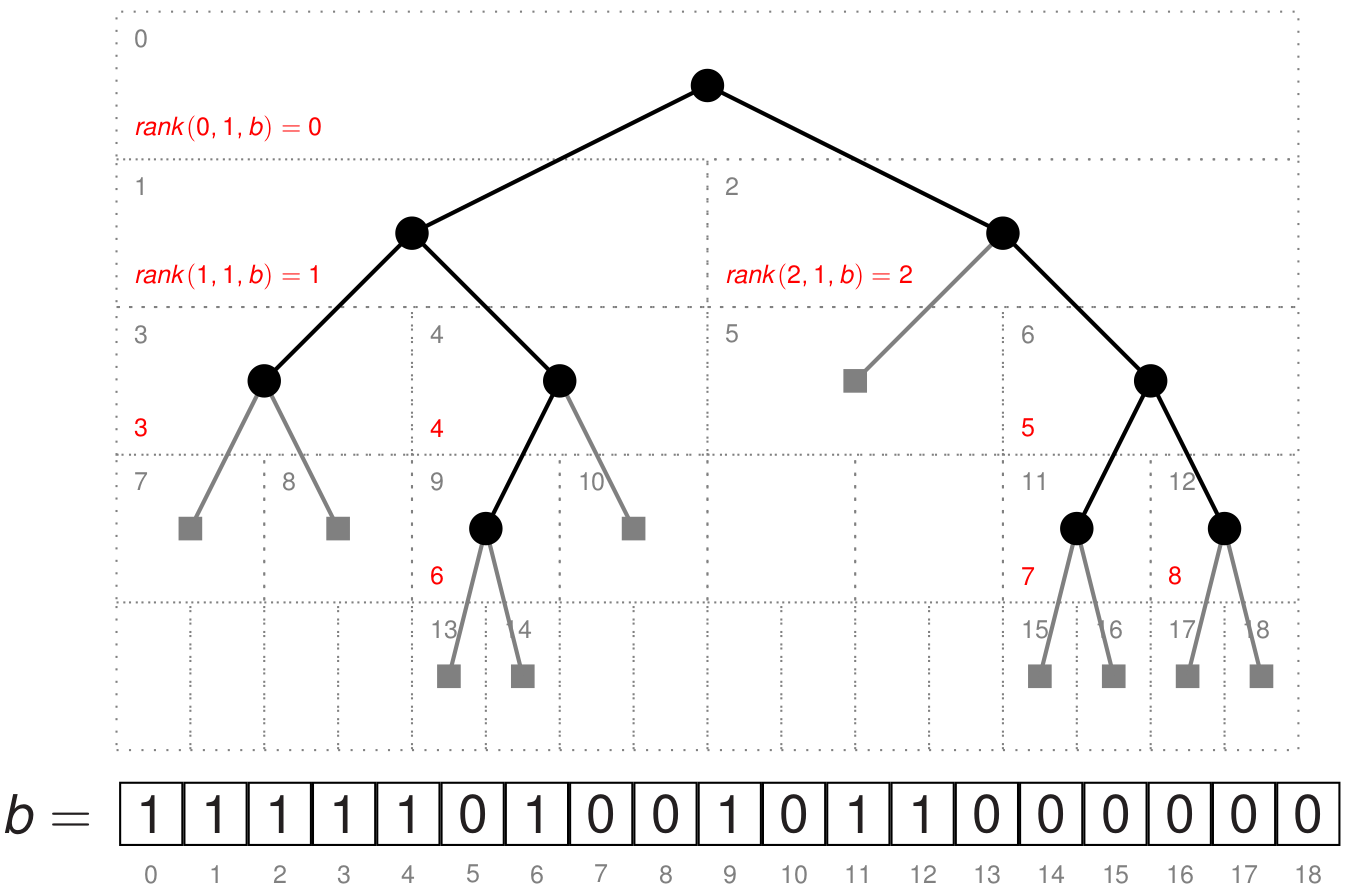
\includegraphics[width=.6\textwidth]{SuccinctBinaryTree2}
  \caption{Jacobson-Kodierung eines Binärbaums}
\end{figure}

Wir können hiermit also einen Binärbaum mit einem Bit-Array der Länge \( 2n + 1 \) (mit \( n \) gesetzten Bits) repräsentieren. Die gewünschten Operationen funktionieren hier so:

\begin{itemize}
  \item \( \text{leftchild}(v) = 2\text{rank}(v) + 1 \)
  \item \( \text{rightchild}(v) = 2\text{rank}(v) + 2 \)
  \item \( \text{parent}(v) =  \) auch in konstanter Zeit möglich\footnote{Übungsaufgabe!}
\end{itemize}

Der totale Platzverbrauch inklusive rank ist also \( 2n + o(n) \) Bits.


\subsection{Bäume --- succinct: LOUDS}

Die Abkürzung \emph{LOUDS} steht für \term{level order unary degree sequence}\index{LOUDS}.

Die Implementierung funktioniert so:

\begin{enumerate}
  \item Füge über der Wurzel des Baums eine Pseudo-Wurzel hinzu und verbinde sie nur mit der alten Wurzel.
  \item Der Ausgangsgrad wird zu jedem Knoten unär\footnote{Ausgangsgrad \( x \): \( x \) mal \texttt{0}, hintendran immer noch eine \texttt{1}.} codiert dazugeschrieben.
\end{enumerate}

Die \term{LOUDS-Sequenz}\index{LOUDS!Sequenz} ist nun die Konkatenantion der Knotenmarkierungen (sortiert nach Level).

\begin{figure}[H]
  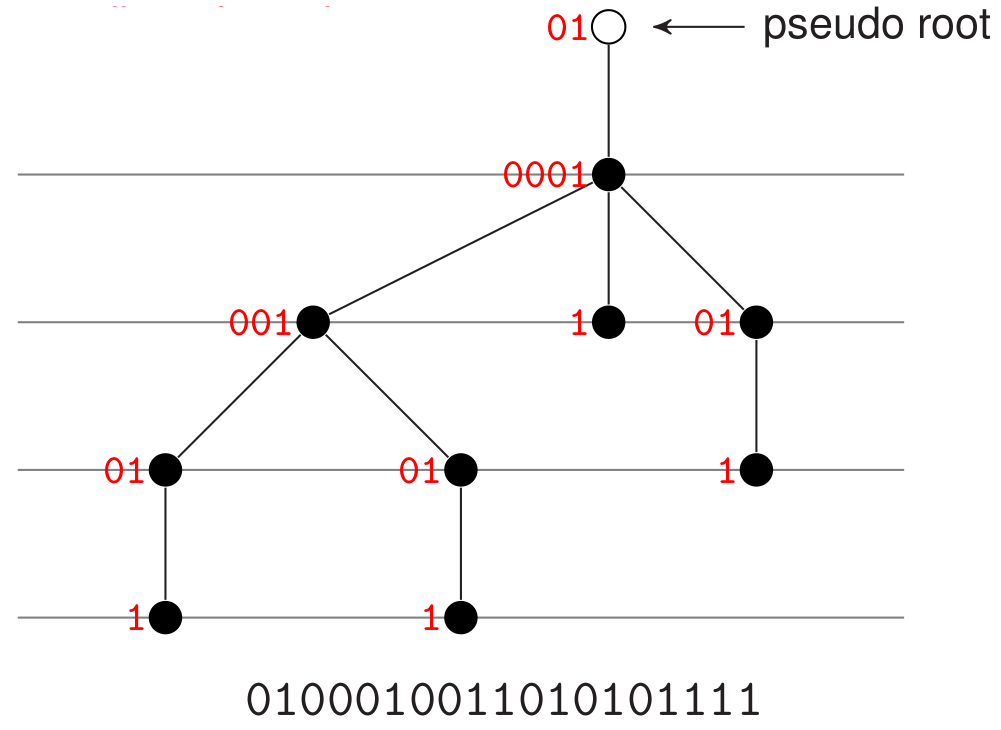
\includegraphics[width=0.5\textwidth]{LOUDS}
  \caption{Allgemeiner Baum mit Pseudo-Wurzel, Knotenmarkierungen und LOUDS-Sequenz}
\end{figure}

Die Konstruktion verursacht, dass --- abgesehen von der Wurzel --- jeder Knoten zweimal in der LOUDS-Sequenz vorkommt: einmal als \texttt{0} in der Kinder-Liste seines Elternknotens und einmal als terminierende \texttt{1} in seiner eigenen Kinder-Liste.

Der gesamte Platzverbrauch hiervorn ist \( 2n + 1 + o(n) \) Bits. Außerdem lassen sich alle gewünschten Operationen in konstanter Zeit implementieren:

\ \\ 

\begin{minipage}{.475\textwidth}
  \begin{pseudocode}
    \textbf{\textsc{isLeaf}}\( (v) \) \\
    id \( \coloneqq \text{rank}(v, 0, \text{LOUDS}) \) \\
    \( p \coloneqq \text{select}(\text{id} + 2, 1, \text{LOUDS}) \) \\
    \textbf{return} \( \text{LOUDS}[p-1] == 1 \) \\
  \end{pseudocode}
\end{minipage}
\hfill
\begin{minipage}{.475\textwidth}
  \begin{pseudocode}
    \textbf{\textsc{outDegree}}\( (v) \) \\
    \textbf{if} \textsc{isLeaf}\( (v) \) \textbf{then return} \( 0 \) \\
    \( \text{id} \coloneqq \text{rank}(v,0,\text{LOUDS}) \) \\
    \textbf{return} \( \text{select}(\text{id}+2,1,\text{LOUDS}) - \) \\ \phantom{\textbf{return}} \( \text{select}(\text{id} + 1, 1, \text{LOUDS}) - 1 \)
  \end{pseudocode}
\end{minipage}

\begin{minipage}{.475\textwidth}
  \begin{pseudocode}
    \textbf{\textsc{child}}\( (v,i) \) \\
    \textbf{if} \( i < \textsc{outDegree}(v) \) \textbf{then} \\ \phantom{\enskip} \textbf{return} \( \perp \) \\
    \( \text{id} \coloneqq \text{rank}(v,0,\text{LOUDS}) \) \\
    \textbf{return} \( \text{select}(\text{id} + 1, 1, \text{LOUDS}) + i \)
  \end{pseudocode}
\end{minipage}
\hfill
\begin{minipage}{.475\textwidth}
  \begin{pseudocode}
    \textbf{\textsc{parent}}\( (v) \) \\
    \textbf{if} \( \textsc{isRoot}(v) \) \textbf{then} \\ \phantom{\enskip} \textbf{return} \( \perp \) \\
    \( \text{pid} \coloneqq \text{rank}(v,1,\text{LOUDS}) \) \\
    \textbf{return} \( \text{select}(\text{pid},0,\text{LOUDS}) \)
  \end{pseudocode}
\end{minipage}
  \chapter{Geometrische Algorithmen}

\begin{tcolorbox}[colframe=black!3!white]
  \textbf{Inhalt dieses Kapitels}:
  \tcblower{} 
  \begin{itemize}
    \item Plane-Sweep-Algorithmus
    \item Konvexe Hülle
    \item Kleinste einschließende Kugel
    \item Range Search
  \end{itemize}
\end{tcolorbox}

\section{Grundlegende Definitionen}

Wir nennen \( p \in \R^d \) einen \term{Punkt}\index{Punkt}. \( p\text{.}i \) stelle die \( i \)-te Komponente von \( p \) dar. Für \( d \in \left \{ 2,3 \right \} \) schreiben wir \( p\text{.}x \), \( p\text{.}y \), \( p\text{.}z \) statt \( p\text{.}1 \), \( p\text{.}2 \), \( p\text{.}3 \).

Für zwei Punkte \( a \), \( b \) definieren wir 
\begin{equation*}
  \overline{ab} \coloneqq \left \{ \alpha *a + (1-\alpha)*b : \alpha \in [0,1] \right \}
\end{equation*}
als das \term{Segment}\index{Segment} zwischen \( a \) und \( b \).

Ein \term{Polygon}\index{Polygon} ist eine Menge an Segmenten, gegeben als Punktemenge \( P = p_1, \dots, p_n \) mit \( p_i \in \R^d \), \( p_n = p_1 \). \( \overline{p_i, p_{i+1}} \) für \( i = 1,\dots,n-1 \) ist der \term{Umriss}\index{Polygon!Umriss} des Polygons.

Ist für alle \( a,b \in P \) auch \( \overline{ab} \in P \), so nennen wir \( P \) \term{konvex}\index{Polygon!konvex}.

\section{Streckenschnitte}

Bei diesem Problem sind \( n \) Strecken \( S = \left \{ s_1, \dots, s_n \right \} \) gegeben und wir wollen alle Schnittpunkte dieser, also \( \bigcup_{s,t \in S} s \cap t \) berechnen.

Naiv lassen sich diese Streckenschnitte in \( O(n^2) \) berechnen:

\begin{pseudocode}
  \textbf{foreach} \( \left \{ s,t \right \} \subseteq S \) \textbf{do} \\
  \phantom{\enskip} \textbf{if} \( s \cap t \neq \varnothing \) \textbf{then} output \( \left \{ s,t \right \} \)
\end{pseudocode}

Dieser Algorithmus ist für große Datenmengen offensichtlich zu langsam.

Idee ist nun, dass eine (waagerechte) \term{Sweep-Line}\index{Sweep-Line} von oben nach unten läuft. Dabei speichern wir Segmente, die \( l \) schneiden, und finden deren Schnittpunkte. Invariante ist, dass Schnittpunkte oberhalb von \( l \) korrekt ausgegeben wurden.

\subsection{Orthogonale Streckenschnitte}

Zuerst betrachten wir die Vereinfachung, dass nur orthogonale Segmente (also parallel zur \( x \)- oder \( y \)-Achse existieren).

\begin{pseudocode}
  \( T \coloneqq \left\langle  \right\rangle \) SortedSequence \textbf{of} Segment \\
  \textbf{invariant} \( T \) stores vertical segments intersecting \( l \) \\
  \( Q \coloneqq \text{sort}(\left\langle (y,s) : \exists \text{ hor-seg } s \text{ at } y \ \vee \ \exists \text{ ver-seg } s \text{ starting/ending at } y \right\rangle) \) \\
  \textbf{foreach} \( (y,s) \in Q \) in descending order \textbf{do} \\
  \phantom{\enskip} \textbf{if} \phantom{\enskip} \( s \) is ver-seg and \emph{starts} at \( y \) \textbf{then} \( T \).insert(\( s \)) \\
  \phantom{\enskip} \textbf{elif} \( s \) is ver-seg and \emph{ends} at \( y \) \textbf{then} \( T \).remove(\( s \)) \\
  \phantom{\enskip} \textbf{else} \phantom{\enskip} \textcolor{gray}{// horizontal segment \( s = \overline{(x_1,y)(x_2,y)} \)} \\
  \phantom{\enskip} \phantom{\enskip} \textbf{foreach} \( t = \overline{(x, y_1)(x,y_2)} \in T \) with \( x \in [x_1, x_2] \) \textbf{do} output \( \left \{ s,t \right \} \)
\end{pseudocode}

Hier sind \( T \) und \( Q \) die einzigen komplexen Datenstrukturen, die wir benötigen, also sortierte Listen an Segmenten (\( T \) geordnet nach \( x \)-Wert, \( Q \) nach \( y \)).

\texttt{insert} und \texttt{remove} gehen in \( O(\log n) \), die \texttt{rangeQuery} für ein Segment in \( O(\log n + k_s) \) (bei \( k_s \) Schritten mit horizontalem Segment \( s \)). Insgesamt haben wir also
\begin{equation*}
  O(n\log n + \sum_s k_s) = O(n\log n + k)\text{.}
\end{equation*}

\subsection{Verallgemeinerung}

Wir verallgemeinern jetzt den Spezialfall von oben, verwenden allerdings folgende Vereinfachungen: Es gebe keine horizontalen Segmente und Überschneidungen sind immer nur zwischen zwei Segmenten, nicht mehr. Außerdem soll es keine Überlappungen geben, die Anzahl an Schnitten zwischen zwei Segmenten ist also immer entweder \( 0 \) oder \( 1 \).

\begin{minipage}{.6\textwidth}
  \vspace*{1em}
  Wir verwenden wieder \( T \) als nach \( x \) geordnete Liste der Strecken, die \( l \) schneidet. Außerdem verwenden wir \emph{Ereignisse} --- diese sind Änderungen von \( T \), also das Starten und Enden von Segmenten sowie Schnittpunkte.

  Einen Schnittest müssen wir nur dann durchführen, wenn zwei Segmente an einem Ereignispunkt in \( T \) benachbart sind.
  \vspace*{1em}
\end{minipage}
\hfill
\begin{minipage}{.35\textwidth}
  \vspace*{1em}
  \begin{figure}[H]
    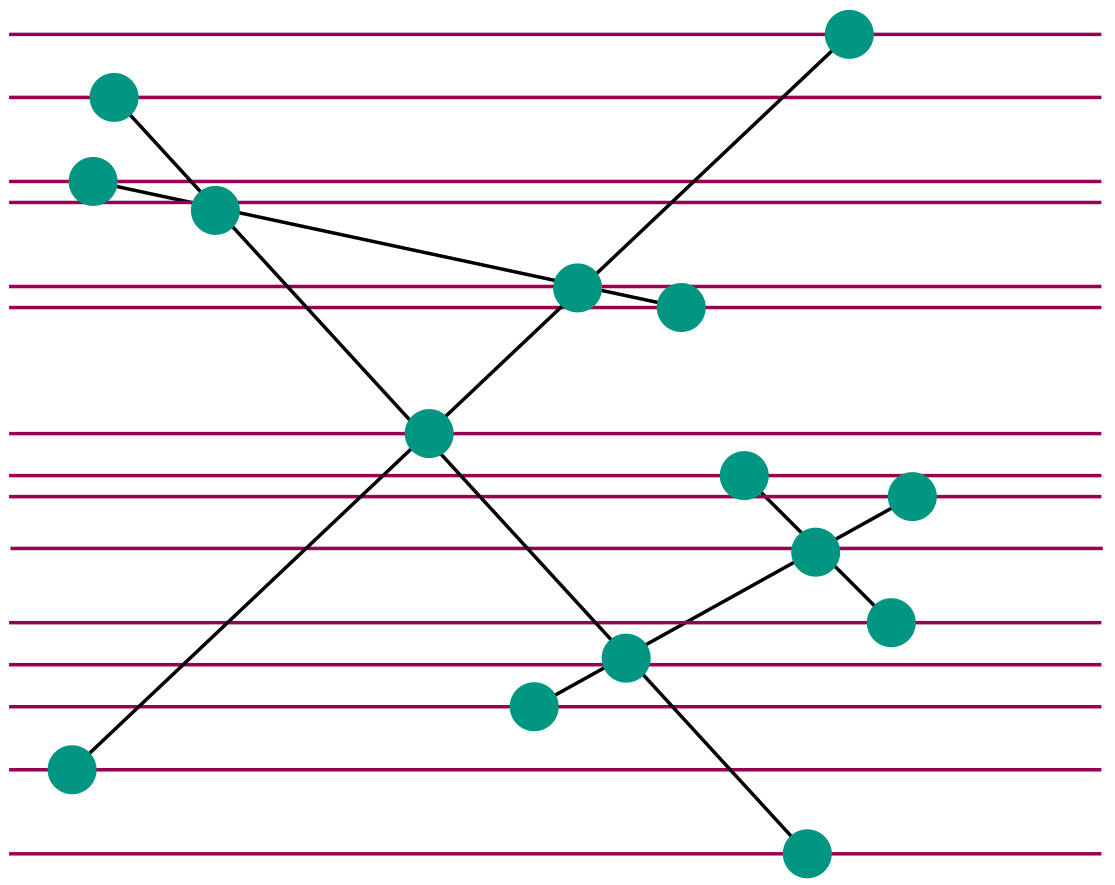
\includegraphics[width=\textwidth]{lineSweep}
    \caption{Die grünen Punkte stellen die Ereignisse dar. Außerdem ist \( l \) zum Zeitpunkt der Ereignisse dargestellt}
  \end{figure}
  \vspace*{1em}
\end{minipage}

Zur Implementierung brauchen wir nun einige Zusatzmethoden:

\begin{minipage}{.35\textwidth}
  \vspace*{1em}
  \textbf{\textsc{findNewEvent}} ermittelt, ob es einen Schnitt zwischen zwei Segmenten \( s \) und \( t \) gibt.
  \vspace*{1em}
\end{minipage}
\hfill
\begin{minipage}{.6\textwidth}
  \vspace*{1em}
  \begin{pseudocode}
    \textbf{\textsc{findNewEvent}}\( (s,t) \) \\
    \textbf{if} \( s \) and \( t \) cross at \( y' < y \) \textbf{then} \\
    \phantom{\enskip} \( Q \).insert(\( (y',\text{intersection},(s,t)) \))
  \end{pseudocode}
  \vspace*{1em}
\end{minipage}

\begin{minipage}{.36\textwidth}
  \vspace*{1em}
  Die Event-Handler werden kümmern sich um die Handhabung der drei möglichen Event-Types.
  \vspace*{1em}
\end{minipage}
\hfill
\begin{minipage}{.6\textwidth}
  \vspace*{1em}
  \begin{pseudocode}
    \textbf{\textsc{handleEvent}}\( (y, \text{\textbf{intersection}}, (a,b), T, Q) \) \\
    output(\( s \cap t \)) \\
    \( T \).swap(\( a \), \( b \)) \\
    \( \text{prev} \coloneqq \text{pred}(b) \) \\
    \( \text{next} \coloneqq \text{succ}(a) \) \\
    findNewEvent(prev, \( b \)) \\
    findNewEvent(\( a \), next)
  \end{pseudocode}
  \vspace*{1em}
\end{minipage}

\begin{minipage}{.475\textwidth}
  \vspace*{1em}
  \begin{pseudocode}
    \textbf{\textsc{handleEvent}}\( (y, \text{\textbf{start}}, s, T, Q) \) \\
    \( h \coloneqq T \).insert(\( s \)) \\
    \( \text{prev} \coloneqq \text{pred}(h) \) \\
    \( \text{next} \coloneqq \text{succ}(h) \) \\
    findNewEvent(prev, \( h \)) \\
    findNewEvent(\( h \), next)
  \end{pseudocode}
  \vspace*{1em}
\end{minipage}
\hfill
\begin{minipage}{.475\textwidth}
  \vspace*{1em}
  \begin{pseudocode}
    \textbf{\textsc{handleEvent}}\( (y, \text{\textbf{finish}}, s, T, Q) \) \\
    \( h \coloneqq T \).locate(\( s \)) \\
    \( \text{prev} \coloneqq \text{pred}(h) \) \\
    \( \text{next} \coloneqq \text{succ}(h) \) \\
    \( T \).remove(\( s \)) \\
    findNewEvent(prev, next)
  \end{pseudocode}
  \vspace*{1em}
\end{minipage}

Nun können wir den Algorithmus implementieren.

\begin{pseudocode}
  \( T \coloneqq \left\langle  \right\rangle \) SortedSequence \textbf{of} Segment \\
  \textbf{invariant} \( T \) stores relative order of segments intersecting \( l \) \\
  \( Q \coloneqq \) MaxPriorityQueue \\
  \( Q \coloneqq Q \cup \left \{ \left( \max\left \{ y,y' \right \}, \text{start}, s \right) : s = \overline{(x,y)(x',y')} \in S \right \} \) \\
  \( Q \coloneqq Q \cup \left \{ \left( \min\left \{ y,y' \right \}, \text{finish}, s \right) : s = \overline{(x,y)(x',y')} \in S \right \} \) \\
  \textbf{while} \( Q \neq \varnothing \) \textbf{do} \\
  \phantom{\enskip} \( (y,\text{type},s) \coloneqq Q \text{.deleteMax} \) \\
  \phantom{\enskip} handleEvent(\( y,\text{type},s,T,Q \))
\end{pseudocode}

Dieser Algorithmus benötigt \( O(n\log n) \) zur Initialisierung und \( O((n+k)\log n) \) für die Event-Schleife, insgesamt also \( O((n+k)\log n) \).
  \chapter{Online-Algorithmen}

\begin{tcolorbox}[colframe=black!3!white]
  \textbf{Inhalt dieses Kapitels}:
  \tcblower{} 
  \begin{itemize}
    \item Einführung in Online-Algorithmen
    \item Beispiel: Job-Scheduling
    \item Beispiel: Skiausleihe
    \item Beispiel: Speicherverwaltung
    \item Beispiel: Auswahl von Experten
  \end{itemize}
\end{tcolorbox}

\term{Online-Algorithmen}\index{Online-Algorithmus} werden verwendet, wenn Eingabegrößen nicht im Vornerein bekannt sind. Viele Algorithmen, die wir bisher diskutiert haben, benötigen Vorarbeitszeit, um optimale Ergebnisse liefern zu können, und sind daher nicht auf Probleme anwendbar, wo die Eingabe in serieller Natur vorliegt. Die bisher diskutierten Algorithmen werden daher auch \term{Offline-Algorithmen}\index{Offline-Algorithmus} genannt.

\section{Übersicht}

Wir werden uns im Folgenden Konzepte von Online-Algorithmen anhand von Beispielen anschauen. Zuerst definieren wir, was ein Online-Algorithmus formal ist.

\begin{itemize}
  \item \textbf{Eingabe}: Folge von Anforderungen (\emph{requests})
  \begin{equation*}
    \sigma = \left( r_1,\dots, r_n \right) \in R^n
  \end{equation*}
  \item \( r_i \) muss auf Anforderung bearbeitet werden, es entsteht eine Antwort
  \begin{equation*}
    a_i = g_i(r_1, \dots,r_i) \in A\text{.}
  \end{equation*}
  Es sind keine Informationen über die Zukunft verfügbar (\( r_{i+1},\dots \)). Antworten sind unwiderruflich.

  Der konkrete Algorithmus ist also durch \( g_1,\dots \) eindeutig festgelegt.

  \item \textbf{Kosten} \( \text{cost}_n : R^n \times A^n \to \R_{> 0} \)

  \item \textbf{Ausgabe} für \( \sigma \in R^n \) ist also
  \begin{equation*}
    \textsc{alg}[\sigma] = \left( g_1(r_1),g_2(r_1,r_2),\dots,g_n(r_1,\dots,r_n) \right) \in A^n
  \end{equation*}
  und die Kosten
  \begin{equation*}
    \textsc{alg}(\sigma) = \text{cost}_n(\sigma,\textsc{alg}[\sigma])
  \end{equation*}
\end{itemize}

\subsection{Kompetitive Analyse}

Um einschätzen zu können, wie gut ein Online-Algorithmus ist, vergleichen wir ihn mit einem optimalen Offline-Algorithmus --- das ist die \term{Kompetitive Analyse}\index{Kompetitive Analyse} dieses Online-Algorithmus.

\begin{definition}[c-kompetitiv]
  Ein Online-Algorithmus ist für ein Optimierungsproblem auf Input \( \sigma \) \term{\( c \)-kompetitiv}\index{kompetitiv!c}, falls es einen Offline-Algorithmus OPT gibt, der nach einem Kostenmaß \( \text{OPT}(\sigma) \) eine Optimallösung berechnen kann, sodass für den betrachteten Online-Algorithmus ALG und alle Eingabesequenzen \( \sigma \) gilt:
  \begin{equation*}
    \text{ALG}(\sigma) \leq c*\text{OPT}(\sigma) + \alpha\text{.}
  \end{equation*}
  Ist die zusätzliche Konstante \( \alpha \leq 0 \), dann heißt ALG \term{strikt \( c \)-kompetitiv}\index{kompetitiv!strikt c}. 

  Unterschied ist, dass man bei nicht-strikter kompetitivität Ausnahmen erlaubt.
\end{definition}

Wir können nun den \term{Wettbewerbsfaktor}\index{Wettbewerbsfaktor} (\emph{competitive ratio}) für den Algorithmus ALG definieren als

\begin{equation*}
  c_{\textsc{alg}} = \sup\left \{ \frac{\textsc{alg}(\sigma)}{\textsc{opt}(\sigma)} : \sigma \in R^+ \right \}\text{.}
\end{equation*}

Ist alg ein strikt \( c \)-kompetitiver Online-Algorithmus und
\begin{equation*}
  C = \left \{ c : \text{\textsc{alg} ist strikt \( c \)-kompetitiv} \right \}\text{,}
\end{equation*}
so ist
\begin{equation*}
  c_\textsc{alg} = \inf C \quad \text{und} \quad c_\textsc{alg} \in C\text{.}
\end{equation*}

Im Folgenden geben wir eine kurze Übersicht über die Beispiele, die wir im Folgenden behandeln werden.

\subsection{Job-Scheduling}

Dieses Beispiel ist dem Beispiel im Kapitel ``Approximationsalgorithmen'' sehr ähnlich. Wir haben
\begin{itemize}
  \item \textbf{Maschinen} \( M_1,\dots,M_m \)
  \item \textbf{Anfrage}: Job \( J_i \), benötigt Zeit \( t_i \geq 0 \)
  \item \textbf{Antwort}: Zuordnung von \( J_i \) zu \( M_j \)
\end{itemize}

Wieder stellt sich die Frage, wie sich der Makespan (also das Intervall zwischen Start und Fertigstellen der letzten Maschine) minimieren lässt. Diese Entscheidung muss hier für jedes \( J_i \) ohne Kenntnis über die zukünftigen Jobs passieren.

\subsection{Skiausleihe}

Die Situation ist hier folgende: Man befinde sich im Skiurlaub und solange das Wetter gut ist, lautet jeden Morgen die \textbf{Anforderung} ``Ski ausleihen!''. Sobald das Wetter allerdings schlecht ist, lautet die \textbf{Anforderung} ``Heimfahren!''.

Es sind zwei \textbf{Antworten} möglich:
\begin{itemize}
  \item Ski für einen Tag ausleihen: Kosten \( k \) Euro
  \item Ski kaufen: Kosten \( K \) Euro (\( K \gg k \))
\end{itemize}

Was muss nun getan werden, um die Gesamtkosten klein zu halten? Diese Entscheidung muss ohne Kenntnis des zukünftigen Wetters gemacht werden!

\subsection{Speicherverwaltung}

``Kosten minimieren'' bedeutet im Speicherverwaltungskontext meist, die Anzahl an Cache Misses zu minimieren. Welche Verdränungsstrategie minimiert die Kosten hier am besten? Und wie kann man am besten zu verdrändende Seiten auswählen, ohne Kenntnis über zukünftige Anforderungen zu haben?

\subsection{Auswahl von Experten}

Hier gibt es mehrere Runden, jede läuft wie folgt ab:
\begin{enumerate}
  \item Jeder von \( n \) Experten gibt zu einer Frage eine Ja/Nein-Empfehlung ab. Diese sind im Allgemeinen nicht richtig.
  \item Man trifft seine eigene Ja/Nein-Entscheidung zu derselben Fragestellung.
  \item Es wird mitgeteilt, welche Entscheidung richtig gewesen wäre.
\end{enumerate}

Wie lässt sich hier die Anzahl an Fehlentscheidungen minimieren?

\subsection{Selbstorganisierende Datenstrukturen}

Hier haben wir eine einfach verkettete Liste und erhalten als \textbf{Anforderung} das Element \( x \) in der Liste. Die dabei entstehenden Kosten sind \( x \). Als \textbf{Reaktion} kann entweder
\begin{itemize}
  \item ohne weitere Kosten das angefragte Element weitrer nach vorne gerückt werden, oder
  \item mit Kosten von \( 1 \) zwei aufeinanderfolgende Elemente vertauscht werden.
\end{itemize}

Welche Listen-Verwaltung minimiert hier die Kosten? Wie kann ohne Kenntnis über zukünftige Anforderungen sinnvoll umgeordnet werden?

\section{Job-Scheduling}

Wir nehmen den listScheduling-Approximationsalgorithmus und bauen ihn in einen Online-Algorithmus um:

\begin{pseudocode}
  \textbf{\textsc{listScheduling}}\( (n,m,t_{1\dots n}) \) \\
  \textbf{each} \( L_i \coloneqq 0 \) \quad \textcolor{gray}{// load of machine \( 1 \leq i \leq m \)} \\
  \textbf{each} \( S_j \coloneqq 0 \) \quad \textcolor{gray}{// machine for job \( 1 \leq j \leq n \)} \\
  \textbf{for each} \( j \) \textbf{in} range\( (1,n) \) \textbf{do} \\
  \phantom{\enskip} pick \( k \) from \( \left \{ i : L_i \text{ is currently minimal} \right \} \) \\
  \phantom{\enskip} \( S_j \coloneqq k \) \\
  \phantom{\enskip} \( L_k \coloneqq L_k + t_j \) \\
  \textbf{return} \( S \)
\end{pseudocode}

Frühere Analysen ergeben, dass der Wettbewerbsfaktor höchstens \( 2 \) ist. Der Online-Algorithmus sieht nun so aus:

\begin{pseudocode}
  \textbf{\textsc{listScheduling}}\( (\phantom{n,}m\phantom{,t_{1\dots n}}) \) \\
  \textbf{each} \( L_i \coloneqq 0 \) \quad \textcolor{gray}{// load of machine \( 1 \leq i \leq m \)} \\
  \phantom{\textbf{each} \( S_j \coloneqq 0 \) \quad \textcolor{gray}{// machine for job \( 1 \leq j \leq n \)}} \\
  \textbf{for each} \( t_j \) \textbf{in} \( \sigma \) \textbf{do} \\
  \phantom{\enskip} pick \( k \) from \( \left \{ i : L_i \text{ is currently minimal} \right \} \) \\
  \phantom{\enskip} \( a_j \coloneqq k \) \\
  \phantom{\enskip} \( L_k \coloneqq L_k + t_j \) \\
  \phantom{\enskip} assign job to machine \( a_j \)
\end{pseudocode}

\section{Skiausleihe}

Wir haben oben bereits diskutiert, was hier das Problem ist.

Die Optimalkosten sind offensichtlich
\begin{itemize}
  \item Falls Urlaubsdauer \( t \leq \frac{K}{k} \) Tage: \( t \) mal ausleihen \( \Rightarrow \) Kosten \( tk \)
  \item Falls Urlaubsdauer \( t > \frac{K}{k} \) Tage: Ski sofort kaufen \( \Rightarrow \) Kosten \( K \)
\end{itemize}

Der Wettbewerbsfaktor ist hier \( 2 \). Optimal ist es, an Tag \( \frac{K}{k} \) die Ski zu kaufen.

% TODO warum? Wird in der Übung gesagt

\section{Speicherverwaltung}

Wir werden uns die folgenden Speicherverwaltungsprobleme anschauen:

\begin{itemize}
  \item \emph{Offline} (lfd ist optimal)
  \item \emph{Deterministisch} (bestenfalls \( k \)-kompetititv)
  \item \emph{Deterministisch}: lru ist \( k \)-kompetititv
  \item \emph{Resource Augmentation}: \( (h,k) \)-Seitenwechsel
  \item \emph{Randomisiert} (randMark ist \( 2H_k \)-kompetititv)
\end{itemize}

Wir betrachten hier stets einen Speicher der Größe \( K \) und einen Cache der Größe \( k \) (\( K \gg k \)).

\subsection{Offline --- lfd ist optimal}

lfd (\emph{longest forward distance}) verdrängt den Eintrag, der am weitesten in der Zukunft benötigt wird. Dieser Algorithmus ist offensichtlich optimal aber auch offensichtlich nicht möglich.

\begin{figure}[H]
  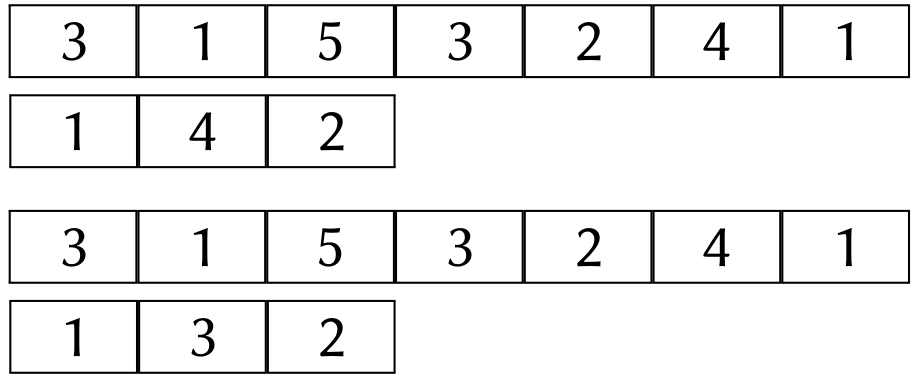
\includegraphics[width=0.4\textwidth]{lfd}
  \caption{Eingabe und Cache vor und nach Bearbeitung der ersten Anforderung. Es wird die \( 4 \) ersetzt, weil sie erst am weitesten in der Zukunft wieder benötigt wird}
\end{figure}

\subsection{Deterministisch --- bestenfalls \( k \)-kompetititv}

Die vier üblichen Algorithmen sind
\begin{itemize}
  \item fifo (\emph{first in first out}),
  \item lifo (\emph{last in first out}),
  \item lru (\emph{least recently used}),
  \item lfu (\emph{least frquently used}).
\end{itemize}

lifo und lfu sind nicht kompetitiv, lru und fifo sind \( k \)-kompetititv. In der Praxis wird üblicherweise lru verwendet.

Es gilt folgender Satz:

\begin{theorem}
  Jeder deterministische Online-Algorithmus für das Seitenwechselproblem mit Cachegröße \( k \) hat einen Wettbewerbsfaktor \( c \geq k \). \( k \) ist also eine untere Schranke für den Wettbewerbsfaktor.
\end{theorem}

\subsection{Deterministisch: lru ist \( k \)-kompetitiv}

Wir können zeigen, dass lru \( k \)-kompetititv ist.

\subsection{Resource Augmentation}

Wir betrachten das \( (h,k) \)-Seitenwechselproblem: hier wird der Online-Algorithmus \( \text{alg}_k \) mit der Cachegröße \( k \) mit \( \text{lfd}_h \) mit Cachegröße \( h < k \) verglichen.

Wir benötigen folgende Definition:

\begin{definition}
  Ein Online-Algorithmus heißt \term{konservativ}\index{Online-Algorithmus!konservativ}, falls er bei Andorderungsfolgen mit höchstens \( k \) verschiedenen Seiten höchstens \( k \) Cache-Misses hat.

  Beispiele hierfür sind lru und fifo.
\end{definition}

Es gilt:
\begin{equation*}
  \text{Jeder konservative Online-Algorithmus ist } \frac{k}{k-h+1} \text{-kompetitiv.}
\end{equation*}

\subsection{Randomisiert: randMark ist \( 2H_k \)-kompetititv}

Bei einem randomisierten Online-Algorithmus zur Speicherverwaltung ist die Zahl der Cache-Misses eine \emph{Zufallsvariable}
\begin{equation*}
  f_R(r_1,\dots,r_n)\text{.}
\end{equation*}

Hier sind gegebenenfalls andere Sichtweisen auf \( c \)-kompetitivität sinnvoll.

Zur Analyse verwenden wir sogenannte \term{Widersacher}\index{Widersacher}. Diese bekommen als Eingabe die gewünschte Länge \( n \) und \( R \) und erzeugen eine ``schlimme'' Anforderungsfolge der Länge \( n \). Diese müssen sie aber auch selbst verarbeiten.

Wir unterscheiden folgende Widersachertypen:

\begin{itemize}
  \item \term{unwissender Widersacher}\index{Widersacher!unwissend} \( W \) (\emph{oblivious adversary}): kein Wissen über erzeugte Zufallsbits, erzeugt für \( (R,n) \) immer gleiches \( (r_1,\dots,r_n) \).
  \item \term{adaptiver Widersacher}\index{Widersacher!adaptiv} \( W' \) (\emph{adaptive adversary}): arbeitet gegen eine konkrete Abarbeitung von \( R \), kennt die von \( R \) bei der Abarbeitung von \( (r_1,\dots,r_i) \) erzeugten Zufallsbits und folglich auch immer den aktuellen Cache-Zustand von \( R \).
\end{itemize}

Wir werden im Folgenden nur unwissende Widersacher analysieren und vergleichen sie mit \( \text{opt}(r_1,\dots,r_n) \).

\begin{definition}
  \( R \) ist \( c \)-kompetitiv gegen unwissende Widersacher, wenn es ein von \( n \) unabhängiges \( b \) gibt, sodass für jede Anforderungsfolge \( (r_1,\dots,r_n ) \) gilt:
  \begin{equation*}
    \textbf{E}[f_R(r_1,\dots,r_n)]-c*\text{opt}(r_1,\dots,r_n) \leq b\text{.}
  \end{equation*}
\end{definition}

Wir betrachten nun den randMark-Algorithmus.\footnote{Fiat et el., 1991}

\begin{pseudocode}
  \( \left\langle \text{Cache: cache}[i]\text{, Markierungsbits mark}[i], 1 \leq i \leq k \right\rangle \) \\
  \textbf{for} \( i \coloneqq 1 \) \textbf{to} \( k \) \textbf{do} mark\( [i] \coloneqq 0 \) \enskip \textcolor{gray}{// alle Markierungen auf \( 0 \)} \\
  \textbf{while} \( \exists \) weitere Anforderungen \textbf{do} \\
  \phantom{\enskip} \( r \coloneqq \) nächste Anforderung \\
  \phantom{\enskip} \textbf{if} \( \text{memory}[r] \not \in \) cache \textbf{then} \\
  \phantom{\enskip} \phantom{\enskip} \textbf{if} \( \forall \text{mark}[i] \equiv 1 \) \textbf{then} \( \forall \text{mark}[i] \coloneqq 0 \) \enskip \textcolor{gray}{// alles \( 1 \leadsto \) neue Phase \( \leadsto \) alles \( 0 \)} \\
  \phantom{\enskip} \phantom{\enskip} \( i \coloneqq \) zufälliges \( j \) mit \( \text{mark}[j] \equiv 0 \) \\
  \phantom{\enskip} \phantom{\enskip} \( \text{cache}[i] \coloneqq \text{memory}[r] \) \\
  \phantom{\enskip} \textbf{else} \( i \coloneqq \) Index mit \( \text{cache}[i] \equiv \text{memory}[r] \) \\
  \( \text{mark}[i] \coloneqq 1 \)

\end{pseudocode}

Dieser Algorithmus ist \( 2H_k \)-kompetitiv gegen unwissende Widersacher.

\section{Auswahl von Experten}

Es gibt mehrere Runden mit folgender Struktur:
\begin{enumerate}
  \item Jeder von \( n \) Experten gibt zu einer Frage eine Ja/Nein-Empfehlung ab. Diese sind im Allgemeinen nicht richtig.
  \item Man trifft seine eigene Ja/Nein-Entscheidung zu derselben Fragestellung.
  \item Es wird mitgeteilt, welche Entscheidung richtig gewesen wäre.
\end{enumerate}

Ziel ist:
\begin{itemize}
  \item \textbf{Anforderung}: \( k \)-Tupel aus Ja/Nein-Empfehlungen der Experten
  \item \textbf{Antwort}: Eigene Ja/Nein-Entscheidung
  \item \textbf{Kosten}: Anzahl eigener Fehlentscheidungen
  \item \textbf{Ziel}: Die eigenen Kosten sollen möglichst nah an den Kosten der besten Experten liegen
\end{itemize}

Es ist leicht einzusehen, dass immer die Antwort des Experten zu wählen, der bisher am meisten korrekte Antworten produziert hat, schlecht ist --- man kann eine Expertenmenge derart konstruieren, dass diese Strategie immer irrt.

\subsection{Weighted Majority Algorithm}

Der \term{Weighted Majority Algorithm}\index{Weighted Majority Algorithm} weist zu Beginn jedem Experte \( i \) ein Gewicht \( w_i \coloneqq 1 \) zu.

In jeder Runde wird die eigene Entscheidung nun folgendermaßen konstruiert:
\begin{enumerate}
  \item Experten geben Empfehlungen \( x_i \in \left \{ \text{ja}, \text{nein} \right \} \)
  \item Eigene Entscheidung fällen:
  \begin{equation*}
    \begin{cases}
      \text{ja,} \quad &\text{falls } \sum_{i,x_i\equiv \text{ ja}}w_i \geq \sum_{i,x_i \equiv \text{nein }}w_i \\
      \text{nein,} \quad &\text{falls } \sum_{i,x_i\equiv \text{ ja}}w_i < \sum_{i,x_i \equiv \text{nein }}w_i
    \end{cases}
  \end{equation*}
  \item Expertengewichte anpassen:
  \begin{equation*}
    w_i^{t+1} = \begin{cases}
      w_i^t\text{,} \quad &\text{falls \( x_i \) richtig war} \\
      \frac{w_i^t}{2}\text{,} \quad &\text{falls \( x_i \) falsch war}
    \end{cases}
  \end{equation*}
\end{enumerate}

wma ist \( \frac{1}{\log_2 (4/3)} \)-kompetitiv. Genauer:
\begin{equation*}
  \text{wma}(\sigma) \leq \frac{1}{\log_2 (4/3)}(\text{optExpert}(\sigma) + \log_2 k)\text{.}
\end{equation*}

\subsection{Verallgemeinerung}

Wir betrachten nun nicht mehr nur den Fall, dass Antworten richtig oder falsch sein können, sondern gewichten sie mit Faktoren zwischen \( 0 \) und \( 1 \). In der \( t \)-ten Runde läuft ab:

\begin{enumerate}
  \item \textbf{Experten}: geben Empfehlungen \( x_1, \dots, x_k \)
  \item Eigene Wahl der Empfehlung
  \item Mitteilung, welche Entscheidung richtig gewesen wäre
  \item Beurteilung der Empfehlungen durch ``Noten'' \( c_i^t \in [0,1] \)
  \item \textbf{Kosten}: Note der gewählten Empfehlung
\end{enumerate}

Wir verwenden hierfür einen randomisierten Algorithmus \( \text{randWMA}_\epsilon \):
\begin{itemize}
  \item Initial:
  \begin{itemize}
    \item Es sei \( \epsilon \in (0,\tfrac{1}{2}) \)
    \item Experte \( i \) hat Gewicht \( w_i \)
    \item alle \( w_i \coloneqq 1 \)
  \end{itemize}
  \item In jeder Runde \( t \):
  \begin{enumerate}
    \item wähle Empfehlung von Experte \( i \) mit Wahrscheinlichkeit
    \begin{equation*}
      p_i = \frac{w_i}{\sum_1^k w_i}
    \end{equation*}
    \item Benotung
    \item setze jedes \( w_i \coloneqq w_i(1-\epsilon c_i^t) \)
  \end{enumerate}
\end{itemize}

Ist \( k \) die Anzahl der Experten und \( 0 < \epsilon < \frac{1}{2} \) und \( \text{randWMA}_\epsilon \) nach einer Anzahl an Runden Gesamtkosten von \( K \) hat und die besten Experten Empfehlungen mit (minimalen) Gesamtkosten \( K_\text{opt} \) gegeben haben, so ist
\begin{equation*}
  K \leq (1+\epsilon)*K_\text{opt} + \frac{\ln n}{\epsilon}\text{.}
\end{equation*}
  \chapter{Parallele Algorithmen}

\section{Einleitung}

Indem man Parallelverarbeitung verwendet, kann man sowohl Ressourcen einsparen als auch Ressourcenrestriktionen brechen:
\begin{itemize}
  \item \textbf{Zeitersparnis}: Arbeiten \( p \) Computer an einem Problem, so sind sie bis zu \( p \) mal so schnell.
  \item \textbf{Kommunikationsersparnis}: Fallen Daten verteilt an, so kann man sie auch verteilt (vor)verarbeiten.
  \item \textbf{Energieersparnis}: Zwei Prozessoren mit halber Taktfrequenz brauchen weniger Energie als ein voll getakteter Prozessor.
  \item \textbf{Speicherbeschränkung}: Mehr Prozessoren haben mehr Hauptspeicher, mehr Cache,\dots
\end{itemize}

Es gibt sehr viele Modelle der Parallelverarbeitung, wir werden hier allerdings nur zwei Standardmodelle diskutieren:
\begin{itemize}
  \item \textbf{Prozessornetzwerke mit} \term{Nachrichtenkopplung}\index{Nachrichtenkopplung}.

    Prozessoren sind hier ``normale CPUs'' mit lokalen Speicher. Gemeinsam mit seinem lokalen Speicher wird eine lokale CPU auch \emph{processing element} (PE) genannt. Der Datenaustausch passiert über ein Netzwerk in Form von Nachrichten zwischen zwei Prozessoren.
  \item \textbf{Parallele Registermaschinen mit} \term{Speicherkopplung}\index{Speicherkopplung}.

    Auch hier wird mit normalen CPUs gearbeitet, allerdings haben diese keinen lokalen Speicher, sondern sind über ein Netzwerk mit Speichermodulen verbunden, auf welche alle CPUs zugreifen können. Der Datenaustausch erfolgt über das Netzwerk zwischen einer CPU und einem Speicher.
\end{itemize}

Auf nachrichtengekoppelte Rechner werden wir genauer eingehen.

\begin{figure}[H]
  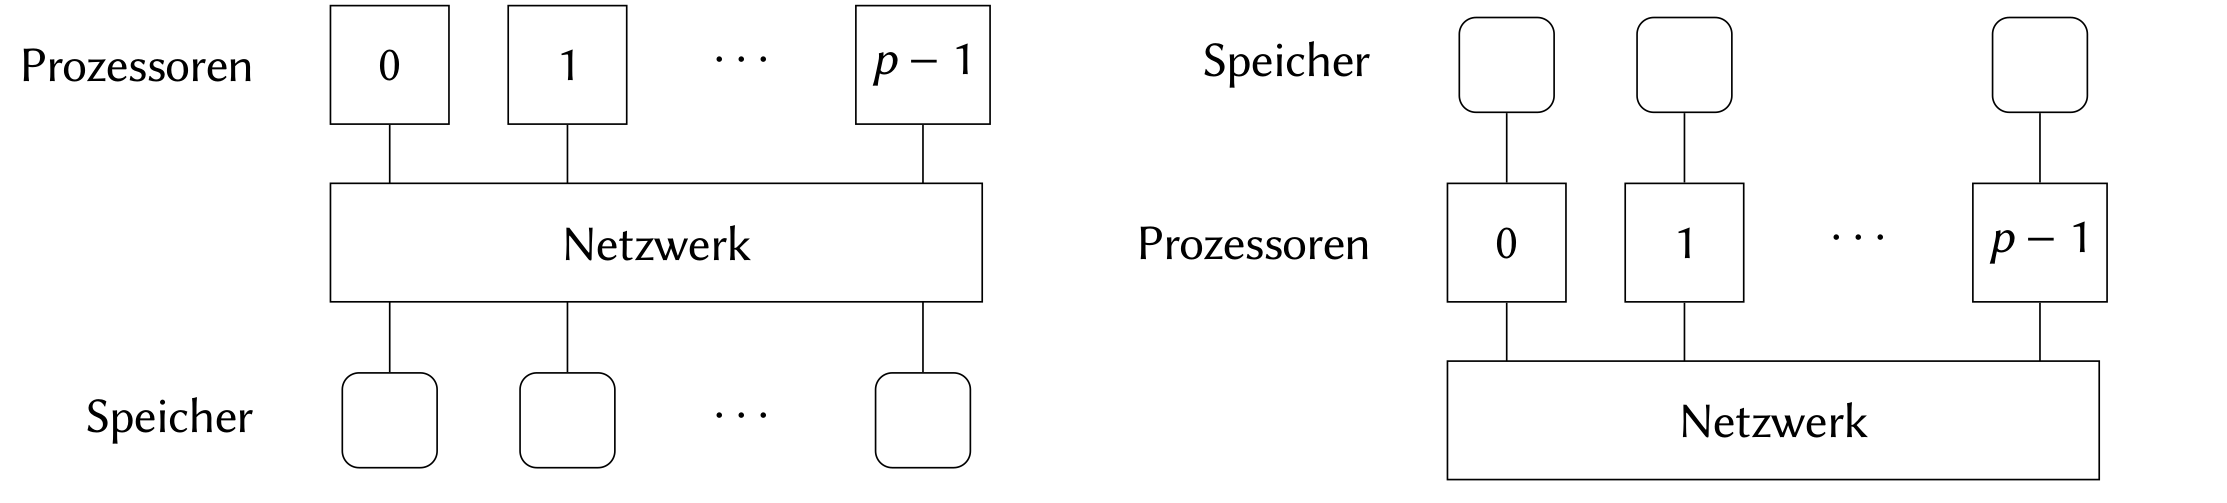
\includegraphics[width=0.9\textwidth]{ParallelArchitectures}
  \caption{Vergleich zwischen \emph{parallelen Registermaschinen mit Speicherkopplung} (links) und einem \emph{Prozessornetzwerk mit Nachrichtenkopplung} (rechts)}
\end{figure}

\subsection{Nachrichtenkopplung vs. Speicherkopplung}

Neben den oben erläuterten Vorteilen von Parallelverarbeitung haben beide Modelle auch Nachteile:

\begin{itemize}
  \item \textbf{Nachrichtenkopplung}:
  \begin{itemize}
    \item Zwei Prozessoren werden zum Datentransport benötigt. Das passt dem Empfänger nicht immer.
    \item Parallelismus muss explizit programmiert werden.
  \end{itemize}
  \item \textbf{Speicherkopplung}:
  \begin{itemize}
    \item \emph{Skalierbarkeit}: Ist eine große Anzahl an Prozessoren sinnvoll?
    \item \emph{Kostenmaß} bei Speicherzugriffskonflikten?
  \end{itemize}
\end{itemize}

Als eine gute Strategie hat es sich erwiesen, den Entwurf für einen verteilten Speicher durchzuführen, da dieser einen viel breiteren Bereich abdecken kann. Die Implementierung erfolgt dann gegebenenfalls für einen gemeinsamen Speicher.

\section{Nachrichtengekoppelte Parallelrechner}

\subsection{Modell}

\begin{itemize}
  \item \textbf{Netzwerk}: Vollständig verknüpftes Punkt-zu-Punkt-Netzwerk
  \begin{itemize}
    \item voll-duplex
    \item Nachrichten überholen sich nicht
  \end{itemize}
  \item \textbf{Prozessoren}: können jeweils maximal gleichzeitig
  \begin{itemize}
    \item eine Nachricht an einen beliebigen Empfänger senden (send(smsg,to))
    \item eine Nachricht von einem beliebigen Sender empfangen (rmsg \( \coloneqq \) recv(from))
    \item \emph{oder} beides gleichzeitig (rmsg \( \coloneqq \) sendRecv(smsg, to, from))
  \end{itemize}
\end{itemize}

Als \emph{Kostenmodell} für das Senden oder Empfangen von \( l \) Bytes verwenden wir
\begin{equation*}
  T_\text{comm}(l) = T_\text{start} + l*T_\text{byte}\text{,}
\end{equation*}
wobei in der Praxis meist \( T_\text{byte} \ll T_\text{start} \). Ignoriert wird hier unter anderem der ``Abstand'' zwischen Sender und Empfänger.

Als \emph{Programmiermodell} verwenden wir \term{SPMD}\index{SPMD} (\emph{single program multiple data}). Alle PEs führen hier dasselbe Programm aus, unterschieden wird lediglich durch ``Ränge'' der PEs (paarweise verschiedene PE-Nummern).

\subsection{Parallele Reduktion}

Im Folgenden gehen wir über die grundlegenden Werkzeuge, die wir benötigen, um parallele Programme analysieren zu können.

\begin{definition}[Reduktion]
  Sei \( \otimes \) eine binäre, assoziative Operation auf einer Menge \( M \).

  Für \( x = (x_0,\dots,x_{p-1}) \in M \) definieren wir
  \begin{equation*}
    R_\otimes(x) = \bigotimes_{i < p}x_i = x_0 \otimes \cdots \otimes x_{p-1}\text{.}
  \end{equation*}
\end{definition}

Nun gilt folgender Satz:

\begin{theorem}
  Wenn \( \otimes \) eine binäre, assoziative Operation ist und \( p \) Elemente \( x_0,\dots,x_{p-1} \) auf \( p \) PEs verteilt sind, dann kann man \( \bigotimes_{i < p}x_i \) in Zeit \( O(\log p) \) auf PE \( 0 \) berechnen.
\end{theorem}

\begin{figure}[H]
  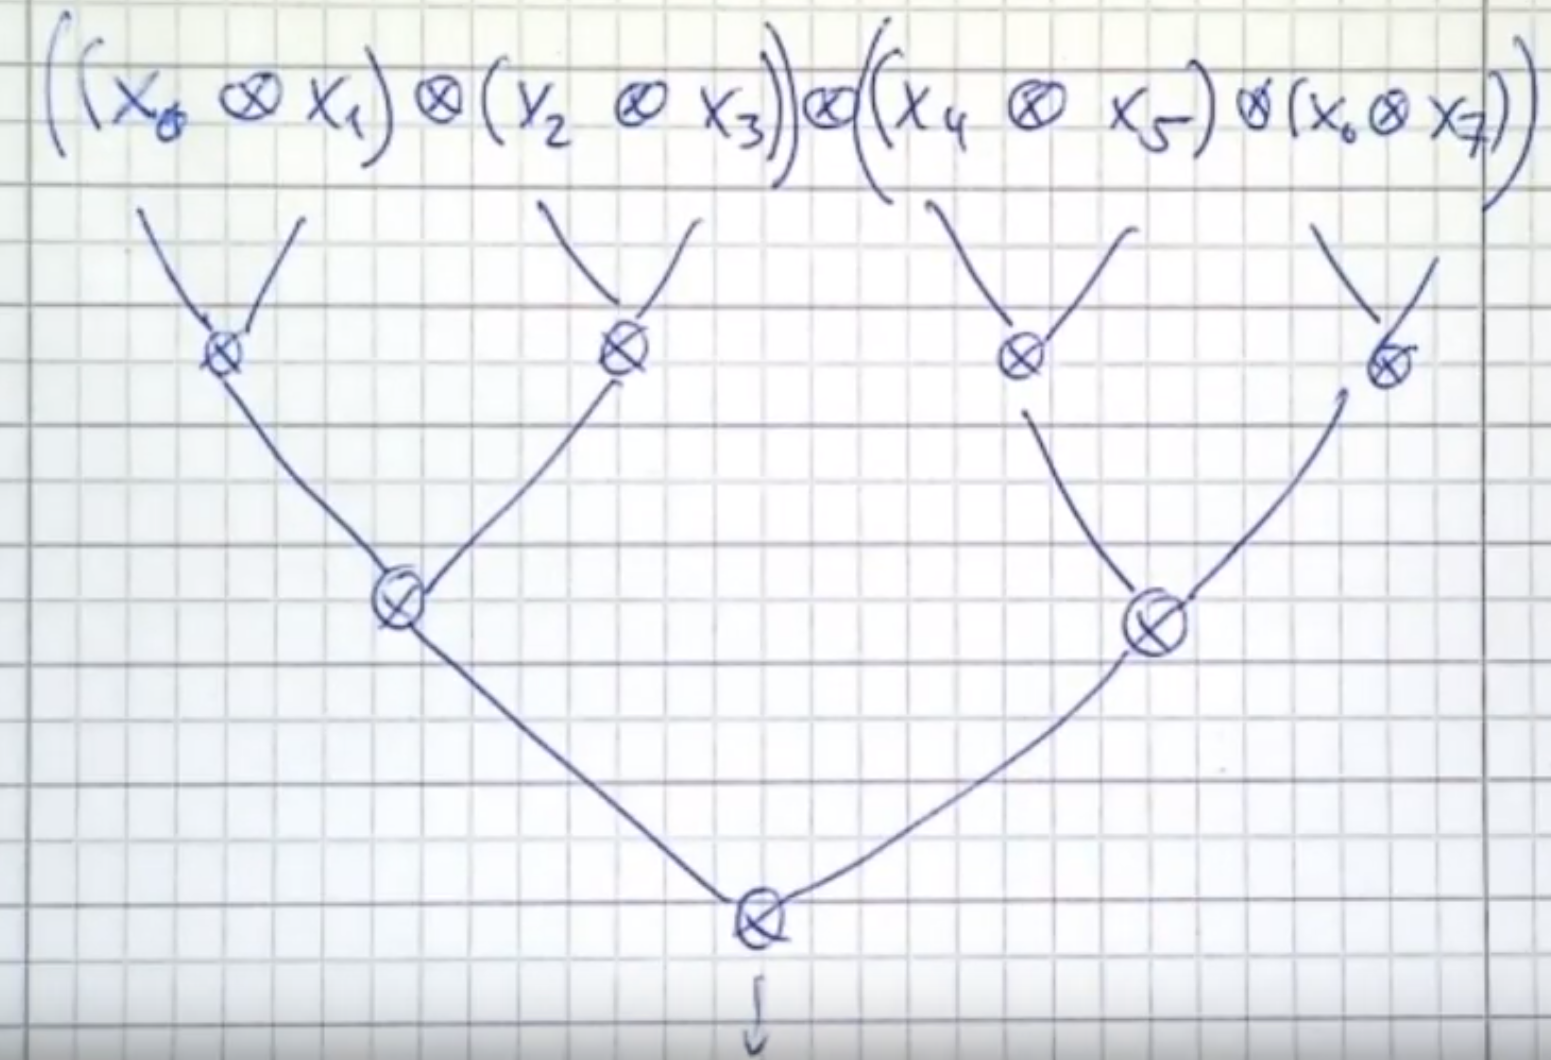
\includegraphics[width=0.6\textwidth]{parallelExecution}
  \caption{Idee hinter obigem Satz}
\end{figure}

Sequenziell wäre die optimale Laufzeit \( O(n) \) gewesen. Auf \( p = n \) PEs hätte man nach obigem Satz eine Laufzeit von \( O(\log n) \) erreicht, also eine Beschleunigung von \( O\left( \frac{n}{\log n} \right) \). ``Ideal'' wäre eine Beschleunigung von \( O(p) = O(n) \) gewesen.

Wie kann man die Beschleunigung noch weiter verbessern?

\subsection{Parallele Reduktion mit \( p < n \)}

Verwenden wir nun \( p < n \) viele PEs, um eine Reduktion auf \( n \) Elementen durchzuführen, so erhält jedes PE \( n/p \) Datenelemente. Die PEs berechnen zuerst die Reduktion der lokalen Elemente, und anschließend wird auf diesen Reduktionen eine parallele Reduktion durchgeführt.
Laufzeit hierfür ist \( O(n/p) + O(\log p) \) und die Beschleunigung somit
\begin{equation*}
  \frac{O(n)}{O(n/p + \log p)}\text{.}
\end{equation*}
Ist \( p \in O(n/\log n) \), so ist die Beschleunigung \( O(p) \).

Man kann also durch Verringerung der Prozessorzahl \( p \) die Beschleunigung in die Nähe von \( p \) bringen. Dieses Prinzip nennt man \term{Brent's Prinzip}\index{Brent's Prinzip}.

\subsection{Analyse paralleler Programme}

Wir interessieren uns in erster Linie für
\begin{itemize}
  \item Laufzeit,
  \item Beschleunigung und
  \item verrichtete Arbeit.
\end{itemize}

Es ist
\begin{itemize}
  \item \( T_\text{par}(I,p) \) die parallele Laufzeit der Probleminstanz \( I \), bearbeitet mit \( p \) PEs,
  \item \( T_\text{seq}(I) \) die sequenzielle Laufzeit der Probleminstanz \( I \) mit dem ``besten bekannten Algorithmus''.
\end{itemize}

Im Allgemeinen ist \( T_\text{seq}(I) < T_\text{par}(I,1) \). Man erhält aber leicht Gleichheit, indem man den parallelen Algorithmus einfach den sequenziellen ausführen lässt, falls nur ein PE zur Verfügung steht.

\begin{definition}[Speedup]
  Wir definieren den \term{Speedup}\index{Speedup} als
  \begin{equation*}
    S(I,p) = \frac{T_\text{seq}(I)}{T_\text{par}(I,p)}\text{.}
  \end{equation*}
  Vergröbert für alle Probleminstanzen der Größe \( n \):
  \begin{equation*}
    S(n,p) = \inf\left \{ S(I,p) : n = \left\vert I \right\vert \right \}\text{.}
  \end{equation*}
\end{definition}

Zur Berechnung des Speedups können wir praktischerweise folgende Spezialfälle benutzen, die für Instanzen \( I \), \( I' \) gleicher Größe \( n \) gelten:
\begin{itemize}
  \item \( T_\text{par}(I,p) = T_\text{par}(I',p) = T_\text{par}(n,p) \),
  \item \( T_\text{seq}(I) = T_\text{seq}(I') = T_\text{seq}(n) \)
\end{itemize}

Simuliert man \( p \) Prozessoren durch einen Prozessor, so sehen wir, dass ein sequenzieller Algorithmus nie langsamer als \( O(p*T_\text{par}(I,p)) \) sein kann, weswegen immer \( \frac{T_\text{seq}(I)}{T_\text{par}(I,p)} \in O(p) \) ist und \( S(n,p) \in O(p) \) ebenfalls.

\begin{definition}[Effizienz]
  Wir definieren die \term{Effizienz}\index{Effizienz} eines parallelen Algorithmus als
  \begin{equation*}
    E(n,p) \coloneqq \frac{S(n,p)}{p}\text{.}
  \end{equation*}
  Es ist \( S(n,p) \in O(p) \) und daher \( E(n,p) \in O(1) \). Tatsächlich ist sogar \( E(n,p) > 1 \) möglich (sogenannter \emph{superlinearer Speedup}).
\end{definition}

Es ist
\begin{equation*}
  E(n,p) \in \frac{T_\text{par}(n,p)}{p*T_\text{seq}(n)}\text{.}
\end{equation*}

\begin{definition}[Arbeit]
  Wir definieren \term{Arbeit}\index{Arbeit} als
  \begin{equation*}
    W(n,p) \coloneqq p*T_\text{par}(n,p) \text{.}
  \end{equation*}
\end{definition}

Mit obiger Definition gilt
\begin{equation*}
  E(n,p) = \frac{S(n,p)}{p} = \frac{T_\text{seq}(n)}{T_\text{par}(n,p)*p} = \frac{T_\text{seq}(n)}{W(n,p)}\text{.}
\end{equation*}

Wir können nun die parallele Reduktion mit \( p < n \) von vorhin genauer analysieren:
\begin{itemize}
  \item Es werden zuerst \( \tfrac{n}{p} \) Elemente sequenziell und anschließend \( p \) partielle Summen reduziert.
  \item \textbf{Laufzeit}: \( T_\text{par}(n,p) = O(n/p) + O(\log p) \)
  \item \textbf{Beschleunigung}: \( S(n,p) = \frac{O(n)}{O(n/p + \log p)} \)
  \item \textbf{Effizienz}: \( E(n,p) = \frac{O(n)}{O(n+p\log p)} \)
\end{itemize}

Wir betrachten noch die zwei Sonderfälle:
\begin{itemize}
  \item \( p = n \):
  \begin{itemize}
    \item \( S(n,n) \in O\left( \frac{n}{\log n} \right) \)
    \item \( E(n,n) \in O\left( \frac{1}{\log n} \right) \)
  \end{itemize}
  \item \( p \in O\left( \frac{n}{\log n} \right) \):
  \begin{itemize}
    \item \( S(n,p) = O(p) \)
    \item \( E(n,p) = O(1) \)
  \end{itemize}
\end{itemize}

Wir erkennen hier die größere Effizienz für kleinere \( p \) (nach Brents Prinzip).

\subsection{Parallele Präfixsummen}

Wir verwenden \( \otimes \) wie oben definiert. Wir definieren nun
\begin{align*}
  &P_\otimes(x) = y = (y_0,\dots,y_{p-1}) \\
  \text{mit } &y_i = \bigotimes_{k \leq i}x_k\text{.} %\text{ oder } y_i = \bigotimes_{k < i}x_k \text{ falls neutrales Element \( e \).}
\end{align*}
Es ist also \( y_0 = x_0 \) und \( y_{i+1} = y_i \otimes x_{i+1} \).

\subsection{Präfixsummen --- Hyperwürfel-Algorithmus}

Wir machen es uns hier einfach und legen fest, dass \( p = n = 2^d \) (für \( d \in \N \)) und \( \otimes \) kommutativ.

Jede PE erhält nun eine ``Koordinate'' \( 0 \leq i \leq 2^d-1 \). Diese wird als Bitvektor
\begin{equation*}
  i = (i_{d-1}\cdots i_0) \quad \text{mit} \quad i_j \in \left \{ 0,1 \right \}
\end{equation*}
repräsentiert. Hier ist \( i_k \) das \( k \)-te Bit von rechts in \( i \).

Wir erlauben Kommunikation zwischen zwei PE \( i \) und \( i' \) nur, wenn die Hammingdistanz ihrer Bitvektoren \( 1 \) ist, sie sich also nur in einer Stelle unterscheiden. Wir erhalten so einen \emph{Hyperwürfel} aus PEs.

Wir berechnen nun Präfixsummen auf einem solchen Hyperwürfel:

\begin{pseudocode}
  \textbf{\textsc{prefixSum}}\( (x,\otimes) \) \\
  \( y \coloneqq x \) \enskip \textcolor{gray}{// auf PE \( i \) liegt \( x_i \)} \\
  \( s \coloneqq x \) \enskip \textcolor{gray}{// für Summe von Elementen in Unterwürfel} \\
  \textbf{for} \( k \coloneqq 0 \) \textbf{to} \( d - 1 \) \textbf{do} \\
  \phantom{\enskip} \( s' \coloneqq \textsc{sendRecv}(s,i \oplus 2^k, i \oplus 2^k) \) \\
  \phantom{\enskip} \( s \coloneqq s \otimes s' \) \\
  \phantom{\enskip} \textbf{if} \( i_k \equiv 1 \) \textbf{then} \( y \coloneqq y \otimes s' \) \\
  \textcolor{gray}{// auf PE \( i \) liegt \( y_i = x_0 \otimes \cdots \otimes x_i \)}
\end{pseudocode}

Wir erhalten eine Laufzeit
\begin{equation*}
  T_\text{prefix} \in O((T_\text{start} + l * T_\text{byte}) * \log p)\text{.}
\end{equation*}

Diese Laufzeit ist nicht optimal. Wie man sie optimieren kann wird in der Vorlesung ``Parallele Algorithmen'' näher erläutert.

\subsection{Paralleles Sortieren}

Hier gibt es zwei verschiedene Aufgabenvarianten:

\begin{enumerate}
  \item Alle \( n \) Elemente liegen zu Beginn auf PE 0. Deswegen muss jedes Element von PE 0 mindestens einmal angefasst werden. Die Laufzeit ist daher in \( \Omega(n) \).
  \item Je \( n/p \) Elemente liegen zu Beginn auf PE \( i \). Dieser Fall ist wesentlich interessanter.
\end{enumerate}

Zunächst betrachten wir den einfachen Fall \( p = n \) (Prozessor \( i \) hat Eingabeelement \( x_i \)). Wir behalten die Grundidee von Quicksort bei:
\begin{itemize}
  \item Wir wählen ein Element pv als Pivot.
  \item Elemente werden umverteilt:
  \begin{itemize}
    \item kleiner als pv: auf Prozessoren mit kleineren Rängen
    \item größer als pv: auf Prozessoren mit großen Rängen
  \end{itemize}
  \item Parallele Rekursion.
\end{itemize}
  \chapter{Fortgeschrittene Datenstrukturen}

Wir werden uns in diesem Kapitel mit Prioritätslisten beschäftigen. Es gibt noch viele weitere fortgeschrittene Datenstrukturen, z.B.
\begin{itemize}
  \item monotone ganzzahlige Prioritätslisten (später im Kapitel ``kürzeste Wege'')
  \item perfektes Hashing
  \item Suchbäume mit fortgeschrittenen Operationen
  \item externe Prioritätslisten (später im Kapitel ``Externe Algorithmen'')
  \item Geometrische Datenstrukturen (siehe Kapitel ``Geometrische Algorithmen'')
\end{itemize}

\section{Adressierbare Prioritätslisten}

Eine \term{adressierbare Prioritätsliste}\index{Adressierbare Prioritätsliste} muss folgene Funktionen implementieren:

\begin{pseudocode}
  \begin{tabular}{ll}
    \textbf{\textsc{build}}\( (\left \{ e_1,\dots,e_n \right \}) \) & \( M \coloneqq \left \{ e_1,\dots,e_n \right \} \) \\
    \textbf{\textsc{size}} & \textbf{return} \( \left\vert M \right\vert \) \\
    \textbf{\textsc{insert}}\( (e) \) & \( M \coloneqq M \cup \left \{ e \right \} \) \\
    \textbf{\textsc{min}} & \textbf{return} \( \min M \) \\
    \textbf{\textsc{deleteMin}} & \( e \coloneqq \min \); \enskip{} \( M \coloneqq M \setminus \left \{ e \right \} \); \enskip{} \textbf{return} \( e \) \\
    \textbf{\textsc{remove}}\( (h : \text{Handle}) \) & \( e \coloneqq h \); \enskip{} \( M \coloneqq M \setminus \left \{ e \right \} \); \enskip{} \textbf{return} \( e \) \\
    \textbf{\textsc{decreaseKey}}\( (h : \text{Handle}, k : \text{Key}) \) & \( \text{key}(h) \coloneqq k \) \\
    \textbf{\textsc{merge}}\( (M') \) & \( M \coloneqq M \cup M' \)
  \end{tabular}
\end{pseudocode}

Adressierbare Prioritätslisten haben viele Anwendungen, beispielsweise im \emph{Dijkstra-Algorithmus} für kürzeste Wege oder in der Graphpartitionierung. Allgemein lassen sich adressierbare Prioritätslisten gut bei Greedy-Algorithmen verwenden, bei denen sich die Prioritäten (begrenzt) ändern.

\subsection{Datenstruktur}

Als grundlegende Datenstruktur wird ein Wald heap-geordneter Bäume verwendet. Hier wird also der Binary Heap verallgemeinert
\begin{itemize}
  \item Baum \( \to \) Wald
  \item zwei Kindknoten \( \to \) beliebig viele Kindknoten
\end{itemize}

Wir verwenden folgende grundlegende Operationen zur Bearbeitung solcher Wälder:
\begin{itemize}

  \begin{minipage}{.475\textwidth}
    \item \textbf{cut}: Teilbaum ausschneiden und als neuen Baum speichern
  \end{minipage}
  \hfill
  \begin{minipage}{.475\textwidth}
    \begin{figure}[H]
      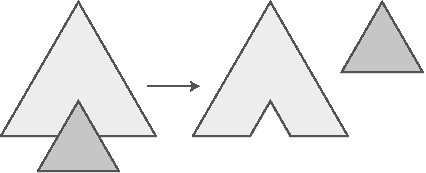
\includegraphics[width=0.8\textwidth]{Cut}
    \end{figure}
  \end{minipage}

  \begin{minipage}{.475\textwidth}
    \item \textbf{link}: Baum 2 mit größerem Wurzelknoten als Baum 1 an Baum 1 als Kindknoten des Wurzelknotens anhängen
  \end{minipage}
  \hfill
  \begin{minipage}{.475\textwidth}
    \begin{figure}[H]
      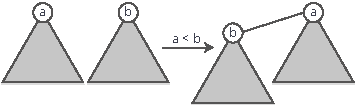
\includegraphics[width=\textwidth]{Link}
    \end{figure}
  \end{minipage}

  \item \textbf{union}: \( \text{union}(a,b) = \text{link}(\min(a,b), \max(a,b)) \)
\end{itemize}

\subsection{Dijkstras Algorithmus}

\term{Dijkstras Algorithmus}\index{Dijkstras Algorithmus} kann die Distanz zwischen einem Startknoten \( s \) und jedem anderen Knoten des Graphen berechnen.

\begin{pseudocode}
  \textbf{\textsc{Dijkstra}}\( (s : \text{Node}, T : \text{Tree}) \) \\
  \textcolor{gray}{// Initialisieren: Distanz zu jedem Knoten ist \( \infty \), zu Startknoten \( 0 \).} \\
  \( d = \left\langle \infty,\ldots,\infty \right\rangle \) \\
  \( d[s] = 0 \) \\
  \textcolor{gray}{// Startknoten zu PQ hinzufügen.} \\
  \( Q\text{.insert}(s) \)
\end{pseudocode}

\begin{itemize}
  \item \( d = \left\langle \infty,\ldots,\infty \right\rangle \)
  
  Zu Beginn ist die Distanz zu jedem Knoten \( \infty \).

  \item \( \text{parent}[s] = s \), \( d(s) = 0 \)
  
  Der Startknoten wird initialisiert.

  \item \( Q\text{.insert}(s) \) 

  Prioritätsliste wird mit Startknoten initialisiert.
\end{itemize}

\section{Pairing Heaps}

\term{Pairing Heaps}\index{Pairing Heaps} müssen folgende Funktionen implementieren:
\begin{pseudocode}
  \textbf{\textsc{insertItem}}\( (h: \text{Handle}) \) \\
  \phantom{\enskip} \( \text{newTree}(h) \) \\
  \textbf{\textsc{newTree}}\( (h: \text{Handle}) \) \\
  \phantom{\enskip} \( \text{forest} \coloneqq \text{forest} \cup \left \{ h \right \} \) \\
  \phantom{\enskip} \textbf{if} \( \ast h < \min \) \textbf{then} \( \text{minPtr} \coloneqq h \) \\
  \textbf{\textsc{decreaseKey}}\( (h : \text{Handle}, k : \text{Key}) \) \\
  \phantom{\enskip} \( \text{key}(h) \coloneqq k \) \\
  \phantom{\enskip} \textbf{if} \( h \) not a root \textbf{then} \( \text{cut}(h) \) \textbf{else} \( \text{updateMinPtr}(h) \) \\
  \textbf{\textsc{deleteMin}}\( () : \text{Handle} \) \\
  \phantom{\enskip} \( m \coloneqq \text{minPtr} \) \\
  \phantom{\enskip} \( \text{forest} \coloneqq \text{forest} \setminus \left \{ m \right \} \) \\
  \phantom{\enskip} \textbf{foreach} child \( h \) of \( m \) \textbf{do} \( \text{newTree}(h) \) \\
  \phantom{\enskip} pairwiseRootUnion\( () \) \\
  \phantom{\enskip} updateMinPtr\( () \) \\
  \phantom{\enskip} \textbf{return} \( m \) \\
  \textbf{\textsc{pairwiseRootUnion}}\( () \) \\
  \phantom{\enskip} \textcolor{gray}{// see picture} \\
  \textbf{\textsc{merge}}\( (o: \text{AdressablePQ}) \) \\
  \phantom{\enskip} \textbf{if} \( \ast\text{minPtr} > \ast(o\text{.minPtr}) \) \textbf{then} \( \text{minPtr} \coloneqq o\text{.minPtr} \) \\
  \phantom{\enskip} \( \text{forest} \coloneqq \text{forest} \cup o\text{.forest} \) \\
  \phantom{\enskip} \( o\text{.forest} \coloneqq \varnothing \)
\end{pseudocode}

Einige Funktionalitäten lassen sich gut veranschaulichen:

\begin{minipage}{.475\textwidth}
  \begin{figure}[H]
    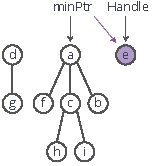
\includegraphics[width=0.5\textwidth]{NewTree}
    \caption{\code{newTree}: Element \( e \) wird hinzugefügt (ggf. auch ein ganzer Baum) und --- falls nötig --- der \code{minPtr} angepasst}
  \end{figure}
\end{minipage}
\hfill
\begin{minipage}{.475\textwidth}
  \vspace{1cm}
  \begin{figure}[H]
    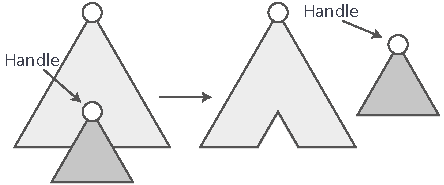
\includegraphics[width=\textwidth]{DecreaseKey}
    \caption{\code{decreaseKey}: Durch Herabsetzen des Keys wird eventuell die Heap-Eigenschaft verletzt, deswegen wird der Teilbaum ausgeschnitten und als neuer Baum hinzugefügt}
  \end{figure}
\end{minipage}

\begin{figure}[H]
  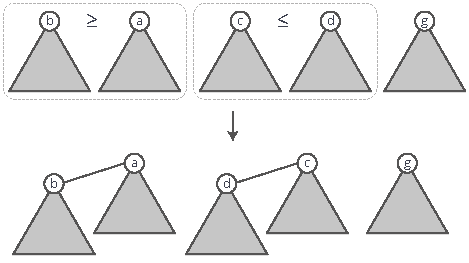
\includegraphics[width=0.6\textwidth]{PairWiseRootUnion}
  \caption{\code{pairwiseRootUnion} fügt jeweils zwei Bäume des Waldes zu einem größeren Baum zusammen, indem die beiden Wurzeln miteinander verglichen werden und eine der beiden Wurzeln Kindknoten der anderen wird}
\end{figure}

\subsection{Repräsentation}

Meistens speichert man Pairing Heaps als doppelt verkettete Liste der Wurzeln. Die Baum-Items können beispielsweise folgendermaßen gespeichert werden:

\begin{figure}[H]
  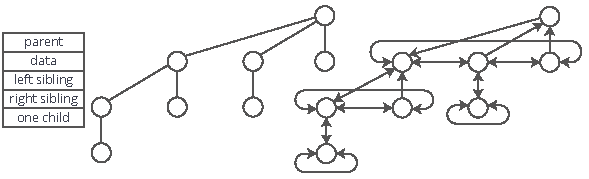
\includegraphics[width=0.8\textwidth]{PairingHeapRepresentation}
  \caption{Speichern der Baum-Items. Man kann hier noch Speicherplatz einsparen, indem man \emph{left sibling} und \emph{parent} zusammenfasst. Allerdings muss man dann alle Geschwisterknoten traversieren, damit man zum Elternknoten kommen kann, da nur der linkeste Kindknoten den Elternknoten speichert}
\end{figure}

\subsection{Analyse}

\begin{itemize}
  \item \code{insert} und \code{deleteMin} gehen in \( O(1) \).
  \item \code{deleteMin} und \code{remove} gehen jeweils in \( O(\log n) \) amortisiert.
  \item \code{decreaseKey} ist schwieriger zu analysieren, geht aber amortisiert in \( O(\log\log n) \leq T \leq O(\log n) \) und ist in der Praxis sehr schnell.
\end{itemize}

Wir werden als nächstes \emph{Fibonacci-Heaps} verwenden, um noch mehr Leistung rauszukitzeln.

\section{Fibonacci-Heaps}

Mithilfe von Fibonacci-Heaps erhalten wir eine amortisierte Komplexität von \( O(\log n) \) für \code{deleteMin} und \( O(1) \) für alle anderen Operationen.

Fibonacci-Heaps speichern ein paar Zusatzinformationen pro Knoten ab, wodurch neue Hilfsfunktionen kreiert werden könnnen, die diese Beschleunigung ermöglichen:

\begin{itemize}
  \item \textbf{Rank} eines Knotens: Anzahl direkter Kinder
  \item \textbf{Mark}: Knoten, die ein Kind verloren haben, werden markiert
  \item \textbf{Vereinigung nach Rank}: Union nur für gleichrangige Wurzeln
  \item \textbf{Kaskadierende Schnitte}: Knoten, die beide markiert sind (also ein Kind verloren haben), werden geschnitten
\end{itemize}

\subsection{Repräsentation}

\begin{minipage}{.725\textwidth}
  Die Repräsentation ist analog zu der von Pairing Heaps, die Wurzeln werden wieder als doppelt verkettete Liste gespeichert und die Baum-Items als Parameterliste:
\end{minipage}
\hfill
\begin{minipage}{.25\textwidth}
  \begin{figure}[H]
    \begin{tabular}{| c |}
      \hline
      parent \\
      \hline
      data, \emph{rank}, \emph{mark} \\
      \hline
      left sibling \\
      \hline
      right sibling \\
      \hline
      one child \\
      \hline
    \end{tabular}
  \end{figure}
\end{minipage}

\subsection{Funktionalität}

\code{insert} und \code{merge} werden wie gehabt implementiert. \code{decreaseKey} verwendet die neue \code{cascadingCut}-Methode und \code{deleteMin} Union-by-Rank. Wir beschleunigen Union-by-Rank, indem wir ein Feld pro Rank bereitstellen und Knoten in diese Felder eintragen. Sollte das passende Feld bereits belegt sein, so wird der neue Knoten mit dem Knoten, der sich im Feld befindet gelinkt und entsprechend verschoben.

\begin{minipage}{.625\textwidth}
  \begin{pseudocode}
    \textbf{\textsc{deleteMin}}\( () : \text{Handle} \) \\
    \phantom{\enskip} \( m \coloneqq \text{minPtr} \) \\
    \phantom{\enskip} \( \text{forest} \coloneqq \text{forest} \setminus \left \{ m \right \} \) \\
    \phantom{\enskip} \textbf{foreach} child \( h \) of \( m \) \textbf{do} \( \text{newTree}(h) \) \\
    \phantom{\enskip} \textbf{while} \( \exists \ a,b \in \text{forest} : \text{rank}(a) \equiv \text{rank}(b) \) \textbf{do} \\
    \phantom{\enskip} \phantom{\enskip} \( \text{union}(a,b) \) \\
    \phantom{\enskip} \( \text{updateMinPtr}() \) \\
    \phantom{\enskip} \textbf{return} \( m \) \\
    \textbf{\textsc{decreaseKey}}\( (h: \text{Handle}, k : \text{Key}) \) \\
    \phantom{\enskip} \( \text{key}(h) \coloneqq k \) \\
    \phantom{\enskip} \( \text{cascadingCut}(h) \) \\
    \textbf{\textsc{cascadingCut}}\( h : \text{Handle} \) \\
    \phantom{\enskip} \textbf{assert} \( h \) is not a root \\
    \phantom{\enskip} \( p \coloneqq \text{parent}(h) \) \\
    \phantom{\enskip} \( \text{unmark}(h) \) \\
    \phantom{\enskip} \( \text{cut}(h) \) \\
    \phantom{\enskip} \textbf{if} \( p \) is marked \textbf{then} \\
    \phantom{\enskip} \phantom{\enskip} \( \text{cascadingCut}(p) \) \\
    \phantom{\enskip} \textbf{else} \( \text{mark}(p) \)
  \end{pseudocode}
  
  Eine amortisierte Analyse von \code{deleteMin} ergibt \( \Omega(\log n) \) für vergleichsbasiertes \code{deleteMin}.
\end{minipage}
\hfill
\begin{minipage}{.35\textwidth}
  \begin{figure}[H]
    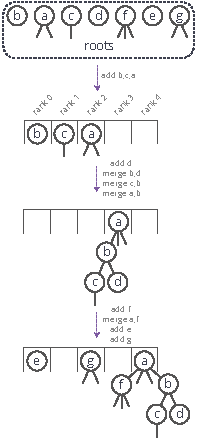
\includegraphics[width=\textwidth]{FastUnionByRank}
    \caption{Fast Union-by-Rank}
  \end{figure}
\end{minipage}
  \chapter{Kürzeste Wege}

Wir betrachten einen Graph \( G = (V,E) \) mit Kantengewicht \( c: E \to \R \) und Anfangsknoten \( s \in V \).

Gesucht ist die Länge \( \mu(v) \) des \term{kürzesten Pfades}\index{Kürzester Pfad} von \( s \) nach \( v \) für alle \( v \in V \), wobei
\begin{equation*}
  \mu(v) \coloneqq \min\left \{ c(p) : p \text{ ist Pfad von \( s \) nach \( v \)} \right \}
\end{equation*}
und
\begin{equation*}
  c\left( \left\langle e_1,\dots,e_k \right\rangle \right) \coloneqq \sum_{i=1}^k c(e_i) \text{.}
\end{equation*}
Oft suchen wir auch eine ``geeignete'' Repräsentation des kürzesten Pfades.

\section{Allgemeine Definitionen}

Wir benutzen im Allgemeinen zwei Knotenarrays:
\begin{itemize}
  \item \( d[v] = \) aktuelle (= vorläufige) Distanz von \( s \) nach \( v \).

  \emph{Invariante}: \( d[v] \geq \mu(v) \).

  \item \( \text{parent}[v] = \) Vorgänger von \( v \) auf (vorläufigem) kürzesten Pfad von \( s \) nach \( v \).

  \emph{Invariante}: Dieser Pfad bezeugt \( d[v] \).
\end{itemize}
Initial ist
\begin{itemize}
  \item \( d[s] = 0 \), \( \text{parent}[s] = s \) und
  \item \( d[v] = \infty \), \( \text{parent}[v] = \perp \).
\end{itemize}
Kern ist das \emph{Relaxieren} der Kanten \( (u,v) \in E \):
\begin{pseudocode}
  \textbf{if} \( d[u] + c(u,v) < d[v] \) \textbf{then} \enskip \textcolor{gray}{// z.B. wenn \( d[v] \equiv \infty \)} \\
  \phantom{\enskip} \( d[v] \coloneqq d[u] + c(u,v) \) \\
  \phantom{\enskip} \( \text{parent}[v] \coloneqq u \)
\end{pseudocode}
Die oben genannten Invarianten werden dadurch nicht verletzt. \( d[v] \) kann sich also problemlos mehrmals ändern.

\section{Dijkstras Algorithmus}

Dijkstras Algorithmus ist der wohl einfachste Algorithmus, um dieses Problem zu lösen. In Pseudocode:

\begin{pseudocode}
  \textcolor{gray}{// \( d \) und parent initialisieren} \\
  \textcolor{gray}{// alle Knoten als ungescannt setzen} \\
  \textbf{while} \( \exists \) non-scanned node \( u \) with \( d[u] < \infty \) \textbf{do} \\
  \phantom{\enskip} \( u \coloneqq \) non-scanned node \( v \) with minimal \( d[v] \) \\
  \phantom{\enskip} relax all edges \( (u,v) \) out of \( u \) \\
  \phantom{\enskip} set \( u \) scanned
\end{pseudocode}

Ist \( v \in V \) von \( s \) aus erreichbar, so wird \( v \) irgendwann gescannt. Wird \( v \) gescannt, so ist \( \mu(v) = d[v] \).

Am Ende definiert \( d \) die optimalen Entfernungen und \code{parent} die zugehörigen Wege. Dieser Algorithmus wurde bereits in Algorithmen I ausführlich diskutiert.

\subsection{Analyse}

Es ist
\begin{equation*}
  T_{\text{Dijkstra}} = O(m*T_\text{decreaseKey}(n) + n*(T_\text{deleteMin}(n) + T_\text{insert}(n)))\text{.}
\end{equation*}
Nutzen wir also Fibonacci-Heaps, so kriegen wir
\begin{equation*}
  T_\text{DijkstraFib} = O(m+n\log n)\text{.}
\end{equation*}

\section{Monotone ganzzahlige Prioritätslisten}

Wir beobachten, dass Dijkstras Algorithmus die Prioritätsliste \emph{monoton} benutzt --- \code{insert} und \code{decreaseKey} benutzen nämlich Distanzen der Form \( d[u] + c(e) \). Die Werte nehmen also ständig zu.

Sind alle Kantengewichte \( \in [0,C] \), so gilt
\begin{equation*}
  \forall v \in V: d[v] \leq (n-1)C\text{.}
\end{equation*}
Ist insbesondere min der letzte Wert, der aus \( Q \) entfernt wurde, so sind in \( Q \) \emph{immer} nur Knoten mit Distanzen im Intervall \( [\min, \min+C] \).

\subsection{Bucket-Queue}

\begin{minipage}{.55\textwidth}
  Eine \term{Bucket-Queue}\index{Bucket-Queue} ist ein zyklisches Array \( B \) von \( C+1 \) doppelt verketteten Listen. Knoten der Distanz \( d[v] \) werden in \( B[d[v] \mod (C+1)] \) gespeichert.  
\end{minipage}
\hfill
\begin{minipage}{.5\textwidth}
  \begin{figure}[H]
    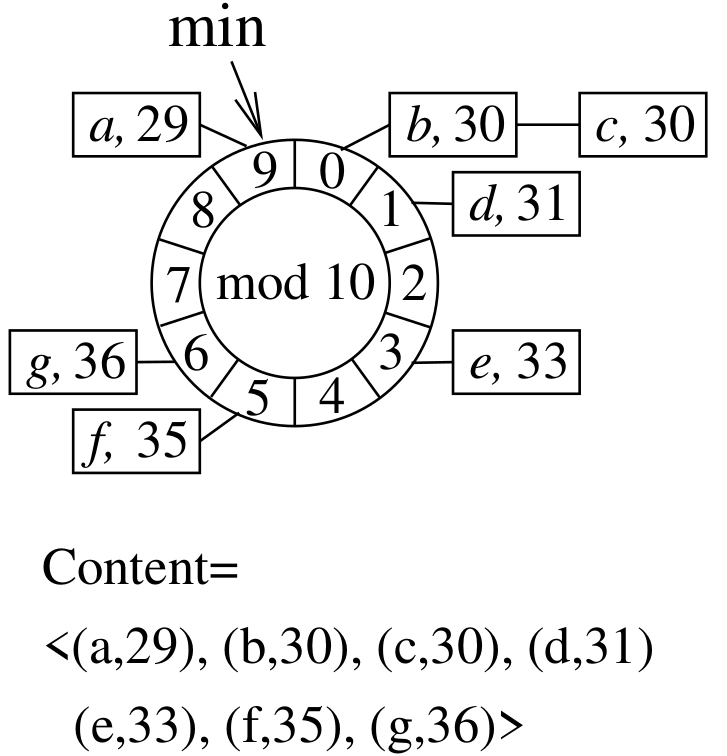
\includegraphics[width=.7\textwidth]{bucketQueue}
    \caption{Bucket-Queue mit \( C = 9 \)}
  \end{figure}
\end{minipage}

Folgende Operationen werden auf einer Bucket Queue implementiert:
\begin{itemize}
  \item \textbf{Initialisierung}: \( C+1 \) leere Listen werden angelegt, \( \min = 0 \).
  \item \textbf{\code{insert(v)}}: fügt \( v \) in \( B[d(v) \text{ mod } (C+1)] \) ein 
  
  \( \Rightarrow O(1) \)

  \item \textbf{\code{decreaseKey(v)}}: schiebt \( v \) von seiner Liste nach \( B[d(v) \text{ mod } (C+1)] \)

  \( \Rightarrow O(1) \)

  \item \textbf{\code{deleteMin}}: fängt bei \( B[\text{min mod } (C+1)] \) an; falls leer, \( \text{min} \coloneqq \text{min}+1 \), \( \circlearrowright \)
  
  \( \Rightarrow O(nC) \)
\end{itemize}

Mit Bucket-Queues kriegen wir also den Dijkstra-Algorithmus auf \( O(m+\text{maxPathLength}) \) gedrückt.

\subsection{Radix-Heaps}

Radix-Heaps sind eine Variante von Bucket Queues, die Buckets von \( -1 \) bis \( K \) für \( K = 1 + \lfloor \log C \rfloor \) benutzt. Wie vorhin schon betrachtet sei \( \min \) die zuletzt aus \( Q \) entfernte Distanz und somit
\begin{equation*}
  \forall v \in Q : d[v] \in [\min,\dots,\min+C]\text{.}
\end{equation*}

Wir betrachten die \emph{binäre Repräsentation} der möglichen Distanzen in \( Q \). Wir speichern \( v \) in Bucket \( B[i] \), falls sich \( d[v] \) und min zuerst an der \( i \)-ten Stelle unterscheiden (Ausnahmen: \( B[K] \) falls \( i > K \), \( B[-1] \) falls sie sich nicht unterscheiden).

Das definiert die \term{Most Significant Digit}\index{Most Significant Digit} (kurz MSD) --- das ist die Position der höchstwertigen Ziffer in der Binärdarstellung von \( a \) und \( b \), an der sich die beiden unterscheiden. \( \text{msd}(a,b) \) kann mit Maschinenbefehlen sehr schnell berechnet werden.

Wir nutzen folgende \emph{Radix-Heap-Invariante}:

\begin{center}
  \( v \) ist gespeichert in Bucket \( B[i] \), wo \( i = \min\left \{ \text{msd}(\min,d[v]),K \right \} \)
\end{center}

Wir können nun \code{deleteMin} folgendermaßen implementieren:

\begin{pseudocode}
  \textbf{\textsc{deleteMin}}\( () : \) Element \\
  \textbf{if} \( B[-1] = \varnothing \) \textbf{then} \\
  \phantom{\enskip} \( i \coloneqq \min\left \{ j \in 0\dots K : B[j] \neq \varnothing \right \} \) \\
  \phantom{\enskip} move \( \min B[i] \) to \( B[-1] \) and to min \\
  \phantom{\enskip} \textbf{foreach} \( e \in B[i] \) \textbf{do} \enskip{} \textcolor{gray}{// exactly here the invariant is violated!} \\
  \phantom{\enskip} \phantom{\enskip} move \( e \) to \( B[\min\left \{ \text{msd}(\min, d[v]), K \right \}] \) \\
  \textbf{return} \( B[-1]\text{.popFront}() \)
\end{pseudocode}

Die \code{deleteMin}-Laufzeit ist \( O(K) \), insgesamt lässt sich also die Laufzeit des Dijkstra-Algorithmus hierdurch auf \( O(m + n\log C) \) drücken.

\section{All-Pairs Shortest Paths}

Herausforderung in diesem Abschnitt ist es, nicht die Abstände zu einem festgelegten Startknoten zu berechnen, sondern zwischen allen Knotenpaaren \( (u,v) \in V^2 \) für \( G = (V,E) \). Zusätzlich erlauben wir negative Kantenkosten, allerdings keine negativen Kreise.

Wir werden zwei verschiedene Lösungen erhalten:

\begin{enumerate}
  \item \( n \) mal den \emph{Bellman-Ford-Algorithmus} ausführen

  \( \Rightarrow O(n^2m) \)

  \item \emph{Knotenpotentiale} verwenden

  \( \Rightarrow O(nm + n^2\log n) \)
\end{enumerate}

\subsection{Bellman-Ford-Algorithmus}

Der \term{Bellman-Ford-Algorithmus}\index{Bellman-Ford-Algorithmus} wurde bereits in Algorithmen I behandelt, deswegen hier nur eine kurze Wiederholung. Wie Dijkstras Algorithmus findet er den kürzesten Pfad zwischen einem festgelegten Startknoten und allen anderen Knoten des Graphen, unterstützt aber auch negative Kantengewichte.

\begin{enumerate}
  \item Distanzen initialisieren: \( d[s] = 0 \), \( d[v] = \infty \) für alle anderen Knoten
  \item Von \( s \) ausgehend alle Knoten des Graphen durchgehen und pro Knoten \( v \) die ausgehenden Kanten betrachten.
  \begin{itemize}
    \item Eintragen, ob \( v \) von \( s \) in \( < \infty \) erreicht werden kann.
    \item Ist \( d[v] + c(v,u) < d[u] \) für einen Nachbar von \( v \)? Wenn ja, \( d[u] \) aktualisieren.
  \end{itemize}
\end{enumerate}

Der zweite Schritt wird maximal \( \left\vert V \right\vert - 1 \) mal wiederholt. Sollte sich schon davor bei einem Durchgang nichts mehr ändern, so kann man aufhören.

Die Laufzeit des Bellman-Ford-Algorithmus ist \( O(nm) \), nutzt man ihn als Basis für All-Pairs Shortest Paths kriegt man also \( O(n * nm) = O(n^2m) \).

\subsection{Knotenpotentiale}

Jeder Knoten erhält ein Potential \( \text{pot}(v) \). Mit diesen Knotenpotentialen lassen sich die \term{reduzierten Kosten} \( \overline{c}(e) \) für eine Kante \( e = (u,v) \in E \) als
\begin{equation*}
  \overline{c}(e) = \text{pot}(u) + c(e) - \text{pot}(v)
\end{equation*}
definieren.

Ist \( p \) ein Pfad von \( u \) nach \( v \) mit Kosten \( c(p) \), dann ist
\begin{equation*}
  \overline{c}(p) = \text{pot}(u) + c(p) - \text{pot}(v)\text{.}
\end{equation*}

Ist \( p' \) ein anderer \( u \)-\( v \)-Pfad, dann gilt
\begin{equation*}
  c(p) \leq c(p') \Leftrightarrow \overline{c}(p) \leq \overline{c}(p')\text{.}
\end{equation*}

Wir berechnen die gewünschten Informationen nun so:
\begin{enumerate}
  \item Wir fügen einen \emph{Hilfsknoten} \( s \) zu \( G \) hinzu.
  \item Wir fügen \( (s,v) \) für alle \( v \in V \setminus \left \{ s \right \} \) mit Kosten \( 0 \) hinzu.
  \item Berechne die kürzesten Pfade von \( s \) aus mit Bellman-Ford.
  \item Definiere \( \text{pot}(v) \coloneqq \mu(v) \) für alle \( v \in V \).

  Die reduzierten Kosten sind jetzt alle nicht-negativ, also können wir Dijkstra benutzen und ggf. \( s \) wieder entfernen.
  \item Für eine beliebige Kante \( (u,v) \in E \) gilt
  \begin{equation*}
    \mu(u) + c(e) \geq \mu(v) \enskip \text{und deshalb} \enskip \overline{c}(e) = \mu(u) + c(e) - \mu(v) \geq 0\text{.}
  \end{equation*}
\end{enumerate}

\begin{pseudocode}
  neuen Knoten \( s \) und alle Kanten \( s,v \) hinzufügen \enskip{} \textcolor{gray}{// \( O(n) \)} \\
  \( \text{pot} \coloneqq \mu \coloneqq \textsc{BellmanFordSSSP}(s,c) \) \enskip{} \textcolor{gray}{// \( O(nm) \)} \\
  \textbf{foreach} \( x \in V \) \textbf{do} \\
  \phantom{\enskip} \( \overline{\mu}(x,\cdot) \coloneqq \textsc{DijkstraSSSP}(x,\overline{c}) \) \\
  \ \\
  \textcolor{gray}{// zurück zur ursprünglichen Kostenfunktion} \\
  \textbf{foreach} \( e = (v,w) \in V^2 \) \textbf{do} \enskip \textcolor{gray}{// \( O(n^2) \)} \\
  \phantom{\enskip} \( \mu(v,w) \coloneqq \overline{\mu}(v,w) + \text{pot}(w) - \text{pot}(v) \)
\end{pseudocode}

Die Gesamtlaufzeit beträgt also \( O(nm + n^2\log n) \).

\section{Distanz zu Zielknoten}

Wir haben bisher zwei Fälle diskutiert:
\begin{enumerate}
  \item Abstände aller Knoten zu einem Startknoten \( s \)
  \item Abstände zwischen allen Knotenpaaren \( \left \{ u,v \right \} \in V^2 \)
\end{enumerate}

Als nächstes schauen wir uns an, wie man den kürzesten Pfad zwischen einem Startknoten \( s \) und einem Zielknoten \( t \) ermittelt.

\subsection{Trick 0 --- Dijkstra abbrechen}

Am einfachsten ist es, einfach Dijkstra abzubrechen, wenn \( t \) aus \( Q \) entfernt wird. Das spart ``im Schnitt'' die Hälfte des Scans.

\subsection{Bidirektionale Suche}

Idee ist hier, abwechselnd von \( s \) und \( t \) aus zu suchen. Von \( s \) aus sucht man auf \( G = (V,E) \), von \( t \) aus auf dem zugehörigen \emph{Rückwärtsgraphen} \( G^r = (V,E^r) \).

Die vorläufige kürzeste Distanz wird in jedem Schritt gespeichert:
\begin{equation*}
  d[s,t] = \min\left \{ d[s,t],d_\text{forward}[u] + d_\text{backward}[u] \right \}
\end{equation*}

Abgebrochen wird, wenn die Suche einen Knoten scannt, der in die andere Richtung bereits gescannt wurde.

\subsection{\( A^\ast \)-Suche}

Idee der \( A^\ast \)-Suche ist es, ``in die Richtung'' des Ziels zu suchen. Dazu benötigen wir eine Funktion \( f(v) \), die für alle \( v \in V \) die eigentliche Funktion \( \mu(v,t) \) schätzen kann.

Anschließend können wir \( \text{pot}(v) = f(v) \) setzen und \( \overline{c}(u,v) = c(u,v) + f(v) - f(u) \).

\( f(v) \) muss diese Eigenschaften haben:
\begin{itemize}
  \item \textbf{Konsistenz}: \( c(e) + f(v) \geq f(u) \) (\( \forall e = (u,v) \)). 

  Die reduzierten Kosten dürfen also nicht negativ sein.

  \item \( f(v) \leq \mu(v,t) \) (\( \forall v \in V \)).

  Dann ist \( f(t) = 0 \) und wir können aufhören wenn \( t \) aus \( Q \) entfernt wird.
\end{itemize}

Ist \( p \) ein beliebiger Pfad von \( s \) nach \( t \), so ist \( d[t] \leq c(p) \) (alle Kanten auf \( p \) seien relaxiert). Wie finden wir jetzt aber so eine Funktion \( f(v) \)?

Wir benötigen eine Heuristik für \( f(v) \).

\begin{itemize}
  \item Betrachtet man eine Strecke im Straßennetzwerk, so kann \( f(v) \) beispielsweise der euklidische Abstand \( \left\Vert v - t \right\Vert_2 \) sein. Damit erhält man eine deutliche, aber keine überragende Beschleunigung.
  \item \term{Landmarks}\index{Landmarks} sind deutlich geeigneter, benötigen allerdings Vorberechnung.

  Man wähle eine \emph{Landmarkmenge} \( L \). Berechne und speichere \( \mu(v,l) \) für alle \( l \in L, v \in V \).

  Während einer Query suche man jetzt ein Landmark \( l \in L \) ``hinter'' dem Ziel und benutze die untere Schranke
  \begin{equation*}
    f_l(v) = \mu(v,l) - \mu(t,l)
  \end{equation*}
  \emph{Vorteile} sind, dass Landmarks konzeptuell einfach sind, eine erhebliche Beschleunigung bringen (um den Faktor 20) und mit anderen Techniken kombinierbar sind.

  \emph{Allerdings} ist die Landmarkauswahl schwierig und der Platzverbrauch sehr groß (besonders für große \( V \)).
\end{itemize}
  \chapter{Anwendungen von DFS}

\section{Starke Zusammenhangskomponenten}

\term{Zusammenhangskomponenten}\index{Zusammenhangskomponente} in einem ungerichteten Graph sind Teilgraphen, in denen es zwischen je zwei beliebigen Knoten einen Pfad gibt.

In gerichteten Graphen sind \term{starke Zusammenhangskomponenten}\index{Zusammenhangskomponente!stark} Teilgraphen \( G \subseteq H \), in denen ebenfalls gilt: für jedes Knotenpaar \( u,v \in G \) gibt es einen \( u \)-\( v \)-Pfad \emph{und} einen \( v \)-\( u \)-Pfad.

Insbesondere werden starke Zusammenhangskomponenten durch Zyklen erzeugt (dann kann man einfach im Kreis laufen von einem Knoten zum anderen). Das bedeutet im Umkehrschluss, dass der \term{Schrumpfgraph}\index{Schrumpfgraph} --- das ist der Graph, den man erhält, indem man jede starke Zusammenhangskomponente als einen Knoten zusammenfasst --- zyklenfrei ist.

\begin{figure}[H]
  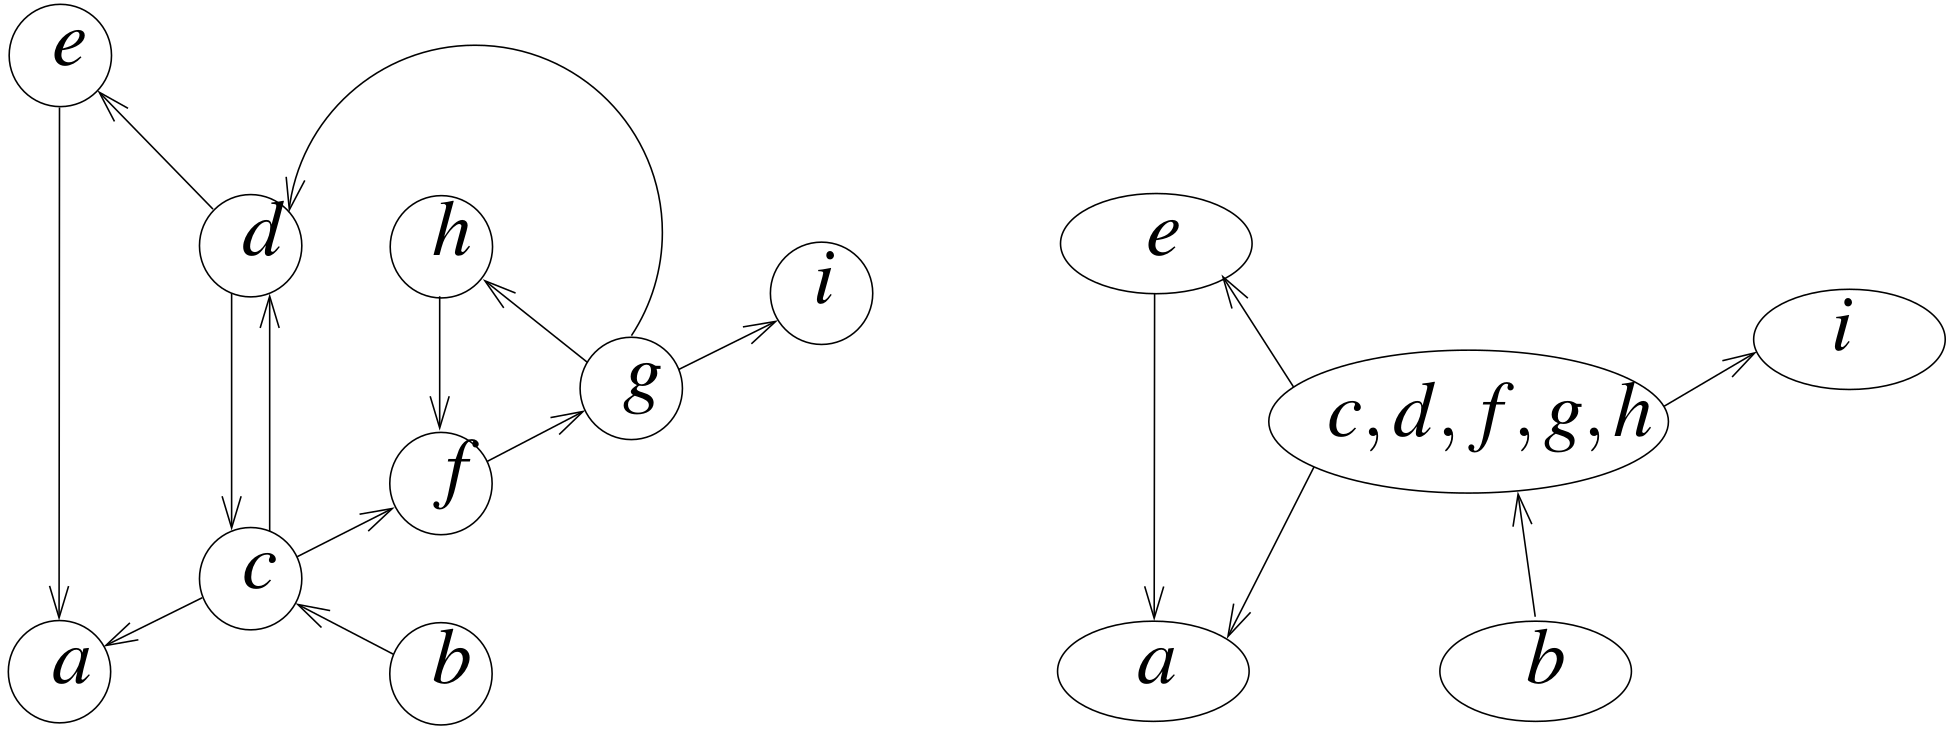
\includegraphics[width=0.6\textwidth]{schrumpfgraph}
  \caption{Gerichteter Graph \( G \) und zugehöriger Schrumpfgraph \( G_S \)}
\end{figure}

\subsection{Tiefensuchschema}

Um später SCCs ermitteln zu können konstruieren wir ein Tiefensuchschema:

\begin{pseudocode}
  unmark all nodes \\
  \textcolor{red}{init}\( () \) \\
  \textbf{foreach} \( s \in V \) \textbf{do} \\
  \phantom{\enskip} \textbf{if} \( s \) is not marked \textbf{then} \\
  \phantom{\enskip} \phantom{\enskip} mark s \\
  \phantom{\enskip} \phantom{\enskip} \textcolor{red}{root}\( (s) \) \\
  \phantom{\enskip} \phantom{\enskip} DFS\( (s,s) \) \\
  \ \\
  \textbf{\textsc{DFS}}\( (u,v : \text{Node}) \) \\
  \phantom{\enskip} \textbf{foreach} \( (v,w) \in E \) \textbf{do} \\
  \phantom{\enskip} \phantom{\enskip} \textbf{if} \( w \) is marked \textbf{then} \\ \phantom{\enskip} \phantom{\enskip} \phantom{\enskip} \textcolor{red}{traverseNonTreeEdge}\( (v,w) \) \\
  \phantom{\enskip} \phantom{\enskip} \textbf{else} \\
  \phantom{\enskip} \phantom{\enskip} \phantom{\enskip} \textcolor{red}{traverseTreeEdge}\( (v,w) \) \\
  \phantom{\enskip} \phantom{\enskip} \phantom{\enskip} mark w \\
  \phantom{\enskip} \phantom{\enskip} \phantom{\enskip} DFS\( (v,w) \) \\
  \phantom{\enskip} \textcolor{red}{backtrack}\( (u,v) \)
\end{pseudocode}

Dieses Tiefensuchschema kann auf unterschiedliche Graphtraversierungsprobleme angepasst werden.

Wir verwenden nun zwei Arrays zum Zwischenspeichern unserer Resultate:
\begin{itemize}
  \item \code{oNodes} speichert die bereits besuchten Knoten,
  \item \code{oReps} speichert die Repräsentanten der einzelnen SCCs.
\end{itemize}

Beim Durchlaufen des Graphen werden die Knoten mit \code{dfsNum} inkrementell durchnummeriert.

Außerdem gibt es drei Invarianten, die wir im Folgenden nicht verletzen dürfen:
\begin{enumerate}
  \item Kanten von abgeschlossenen Knoten gehen zu abgeschlossenen Knoten
  \item Offene Komponenten \( S_1,\dots,S_k \) bilden einen Pfad in \( G_C^s \).
  \item Repräsentanten partitionieren die offenen Komponenten bezüglich ihrer \code{dfsNum}.
\end{enumerate}

Für das Finden von SCCs brauchen wir folgende Implementierungen für die rot gekennzeichneten Prozesuren:
\begin{itemize}
  \item \textbf{\code{root(s)}}:
  \begin{pseudocode}
    oReps.push\( (s) \) \\
    oNodes.push\( (s) \)
  \end{pseudocode}
  Hierdurch wird eine neue offene Komponente gebildet und \( s \) als besucht gekennzeichnet.

  \item \textbf{\code{traverseTreeEdge(v,w)}}:
  \begin{pseudocode}
    oReps.push\( (w) \) \\
    oNodes.push\( (w) \)
  \end{pseudocode}
  Hier wird \( \left \{ w \right \} \) als neue offene Komponente angelegt.

  \item \textbf{\code{traverseNonTreeEdge(v,w)}}:
  \begin{pseudocode}
    \textbf{if} \( w \in \text{oNodes} \) \textbf{then} \\
    \phantom{\enskip} \textbf{while} \( w\text{.dfsNum} < \text{oReps.top.dfsNum} \) \textbf{do} oReps.pop
  \end{pseudocode}
  Ist \( w \not \in \text{oNodes} \) ist \( w \) abgeschlossen und die Kante somit uninteressant. Ist \( w \) allerdings in oNodes, so werden die auf dem Kreis befindlichen SCCs kollabiert.

  \item \textbf{\code{backtrack(u,v)}}:
  \begin{pseudocode}
    \textbf{if} \( v \equiv \text{oReps.top} \) \textbf{then} \\
    \phantom{\enskip} \text{oReps.pop} \\
    \phantom{\enskip} \textbf{repeat} \\
    \phantom{\enskip} \phantom{\enskip} \( w \coloneqq \text{oNodes.pop} \) \\
    \phantom{\enskip} \phantom{\enskip} \( \text{component}[w] \coloneqq v \) \\
    \phantom{\enskip} \textbf{until} \( w = v \)
  \end{pseudocode}
\end{itemize}

Damit haben wir alles was wir brauchen, um die Suche nach SCCs durchführen zu können. Wir kriegen sie sogar in \( O(m+n) \), also in Linearzeit, hin!

\begin{figure}[H]
  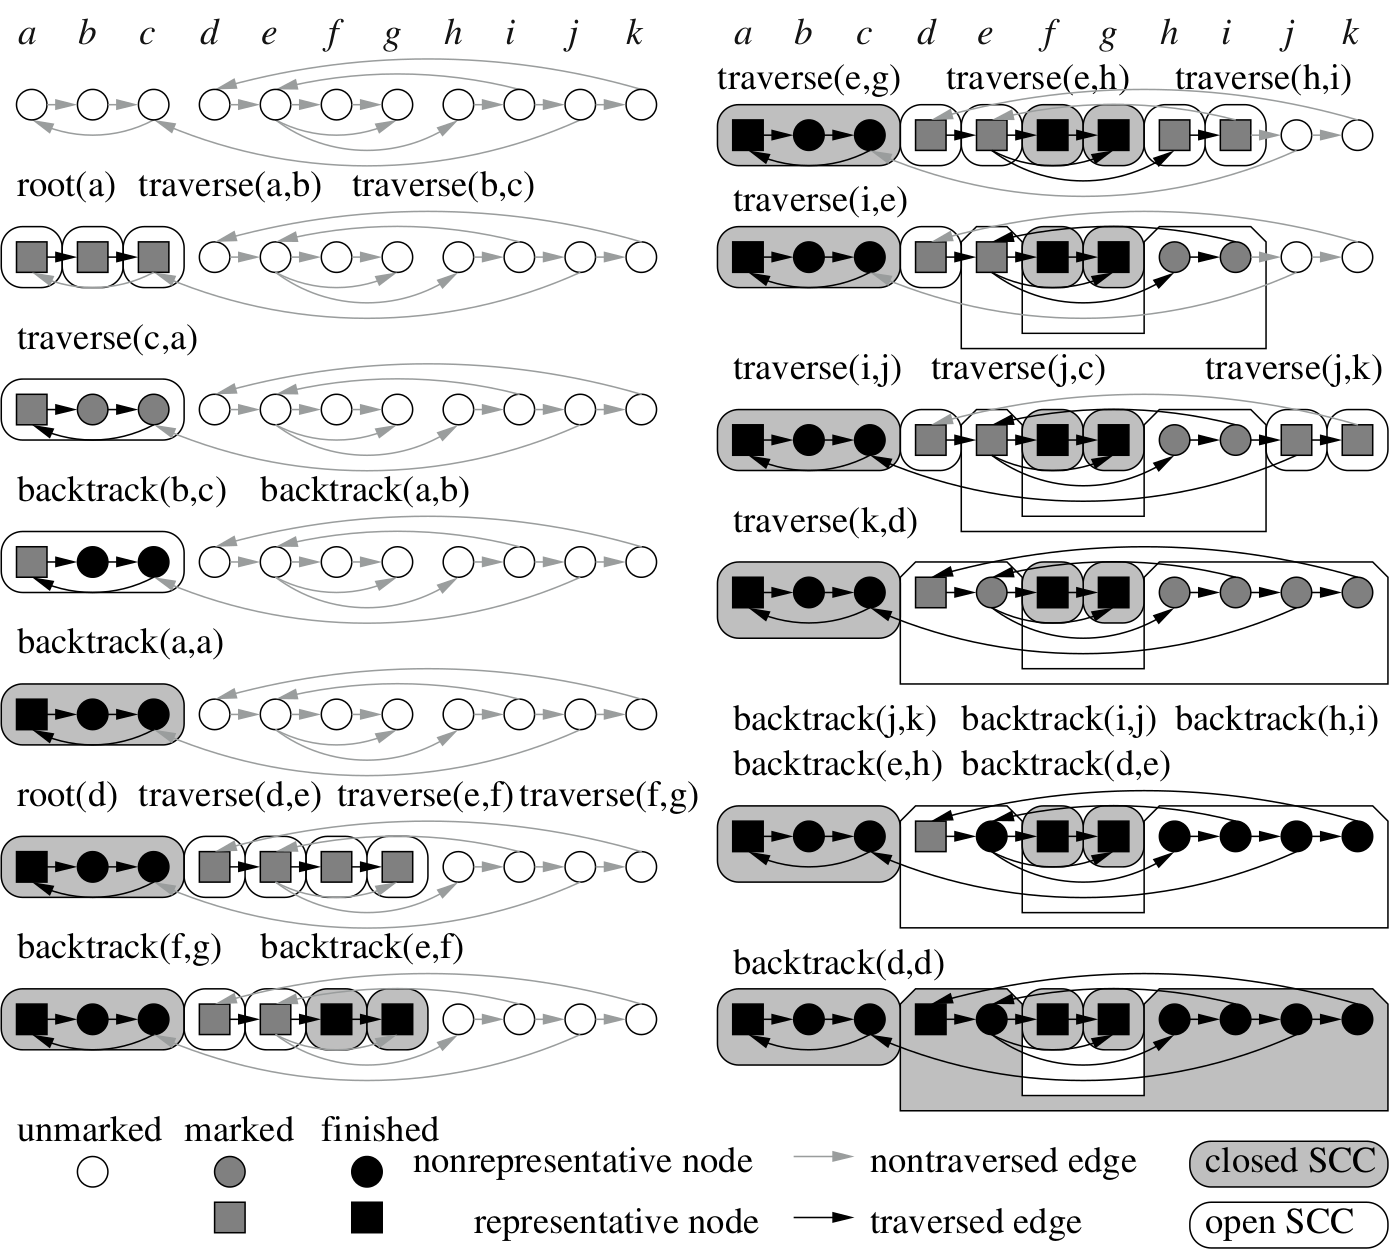
\includegraphics[width=0.6\textwidth]{SCC}
  \caption{Kompletter Durchlauf des Algorithmus}
\end{figure}
  \chapter{Maximale Flüsse und Matchings}

% helpers
\newcommand{\pluseq}{\mathrel{+}=}
\newcommand{\minuseq}{\mathrel{-}=}

\section{Definitionen}

\subsection{Netzwerk}

Ein \term{Netzwerk}\index{Netzwerk} ist ein gerichteter und gewichteter Graph mit zwei speziellen Knoten --- einer \term{Quelle}\index{Netzwerk!Quelle} und einer \term{Senke}\index{Netzwerk!Senke}.

Unterschied zwischen \( s \), \( t \) und dem Rest der Knoten ist, dass \( s \) keine eingehenden und \( t \) keine ausgehenden Kanten hat. 

Das Gewicht \( c_e \) der Kante \( e \) nennen wir die \term{Kapazität}\index{Netzwerk!Kapazität} der Kante. Diese muss nicht-negativ sein.

\begin{figure}[H]
  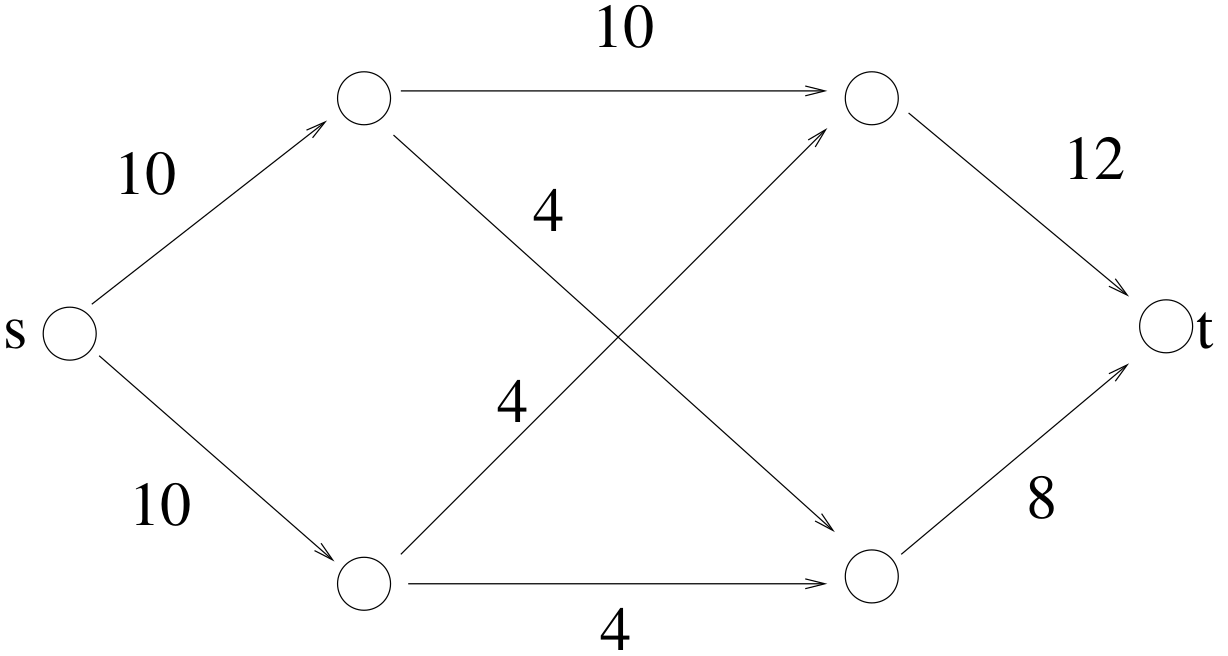
\includegraphics[width=0.6\textwidth]{network}
  \caption{Beispiel für ein Netzwerk mit Quelle \( s \) (\emph{source}) und Senke \( t \) (\emph{sink})}
\end{figure}

\subsection{Fluss}

Ein \term{Fluss}\index{Fluss} in einem Netzwerk ist eine Funktion \( f_e \) auf den Kanten des Netzwerks. Ein Fluss hat folgende Eigenschaften:

\begin{itemize}
  \item \( 0 \leq f_e \leq c_e \) (\( \forall e \in E \))
  \item \( \forall v \in V \setminus \left \{ s,t \right \} : \) Summe eingehender Flüsse = Summe ausgehender Flüsse
\end{itemize}

Wir definieren außerdem den \term{Wert}\index{Fluss!Wert} eines Flusses \( f \) als
\begin{equation*}
  \text{val}(f) = \Sigma \text{ von \( s \) ausgehender Fluss} \equiv \Sigma \text{ zu \( t \) eingehender Fluss}
\end{equation*}

Ziel ist es in der Regel, einen Fluss in einem festgelegten Netzwerk mit \emph{maximalem Wert} zu finden.

\section{Cuts}

\begin{definition}[Cut]
  Ein \( s \)-\( t \)-\term{Cut}\index{Cut} ist eine Partitionierung eines Graphen \( G \) in zwei Mengen \( S \) und \( T \), sodass \( s \in S \) und \( t \in T \).

  Die \term{Kapazität}\index{Cut!Kapazität} eines Cuts ist
  \begin{equation*}
    \sum\left \{ c_{(u,v)} : u \in S \wedge v \in T \right \}\text{,}
  \end{equation*}
  also die Summe der Kapazitäten aller Kanten, die durch den Cut ``durchgeschnitten'' werden.
\end{definition}

\begin{figure}[H]
  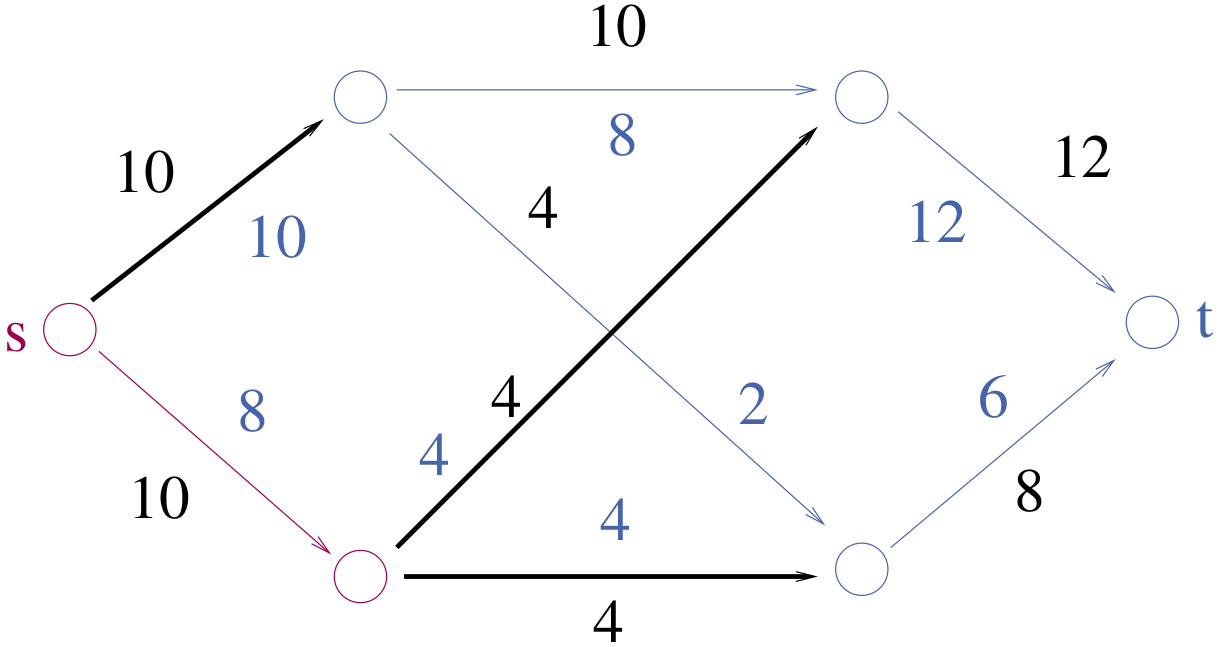
\includegraphics[width=0.6\textwidth]{flow}
  \caption{Die blauen Zahlen stellen einen möglichen Fluss in obigem Netzwerk dar. Die schwarzen Kanten sind ein möglicher Cut. Der Wert dieses Flusses ist 18}
\end{figure}

Es gilt folgender extrem praktischer Satz:

\begin{theorem}[Fluss-Cut-Dualität]
  Der Wert eines maximalen \( s \)-\( t \)-Flusses ist die minimale Kapazität eines \( s \)-\( t \)-Cuts.
\end{theorem}

Wie können wir nun diesen Satz nutzen, um einen maximalen Fluss zu finden? Eine Möglichkeit ist \emph{Lineare Programmierung}, aber es gibt bessere Lösungen.

\section{Pfade augmentieren}

Idee ist folgende:
\begin{enumerate}
  \item Wähle einen \( s \)-\( t \)-Pfad, der noch Kapazität übrig hat.
  \item Sättige die Pfadkante mit der kleinsten Restkapazität.
  \item Korrigiere die Kapazitäten aller anderen Kanten mithilfe des \emph{Residualgraphen} und starte wieder von vorne.
\end{enumerate}

\subsection{Residualgraph}

Ist ein Netzwerk \( G = (V, E, c) \) mit Fluss \( f \) gegeben, so erhalten wir den \term{Residualgraphen}\index{Residualgraph} \( G_f = (V, E_f, c^f) \). Dabei gilt für jedes \( e \in E \):
\begin{equation*}
  \begin{cases}
    e \in E_f \text{ mit } c_e^f = c_e - f(e) \quad &\text{falls } f(e) < c(e)  \\
    e^\text{rev} \in E_f \text{ mit } c_{e^\text{rev}}^f = f(e) \quad &\text{falls } f(e) > 0
  \end{cases}
\end{equation*}
Dabei ist für \( e = (u,v) \in E \) die Kante \( e^\text{rev} = (v,u) \).

Die Kanten in die ``normale'' Richtung sind also diejenigen, die noch Restkapazität haben; die neue Kapazität ist die Restkapazität.

Die Kanten in umgekehrte Richtung sind die Kanten, wo der Fluss \( > 0 \) ist (das heißt insbesondere, dass auch beide Fälle eintreten können). Das Gewicht dieser Kanten entspricht dem Fluss der Kanten in normale Richtung.

\begin{minipage}{.475\textwidth}
  \begin{figure}[H]
    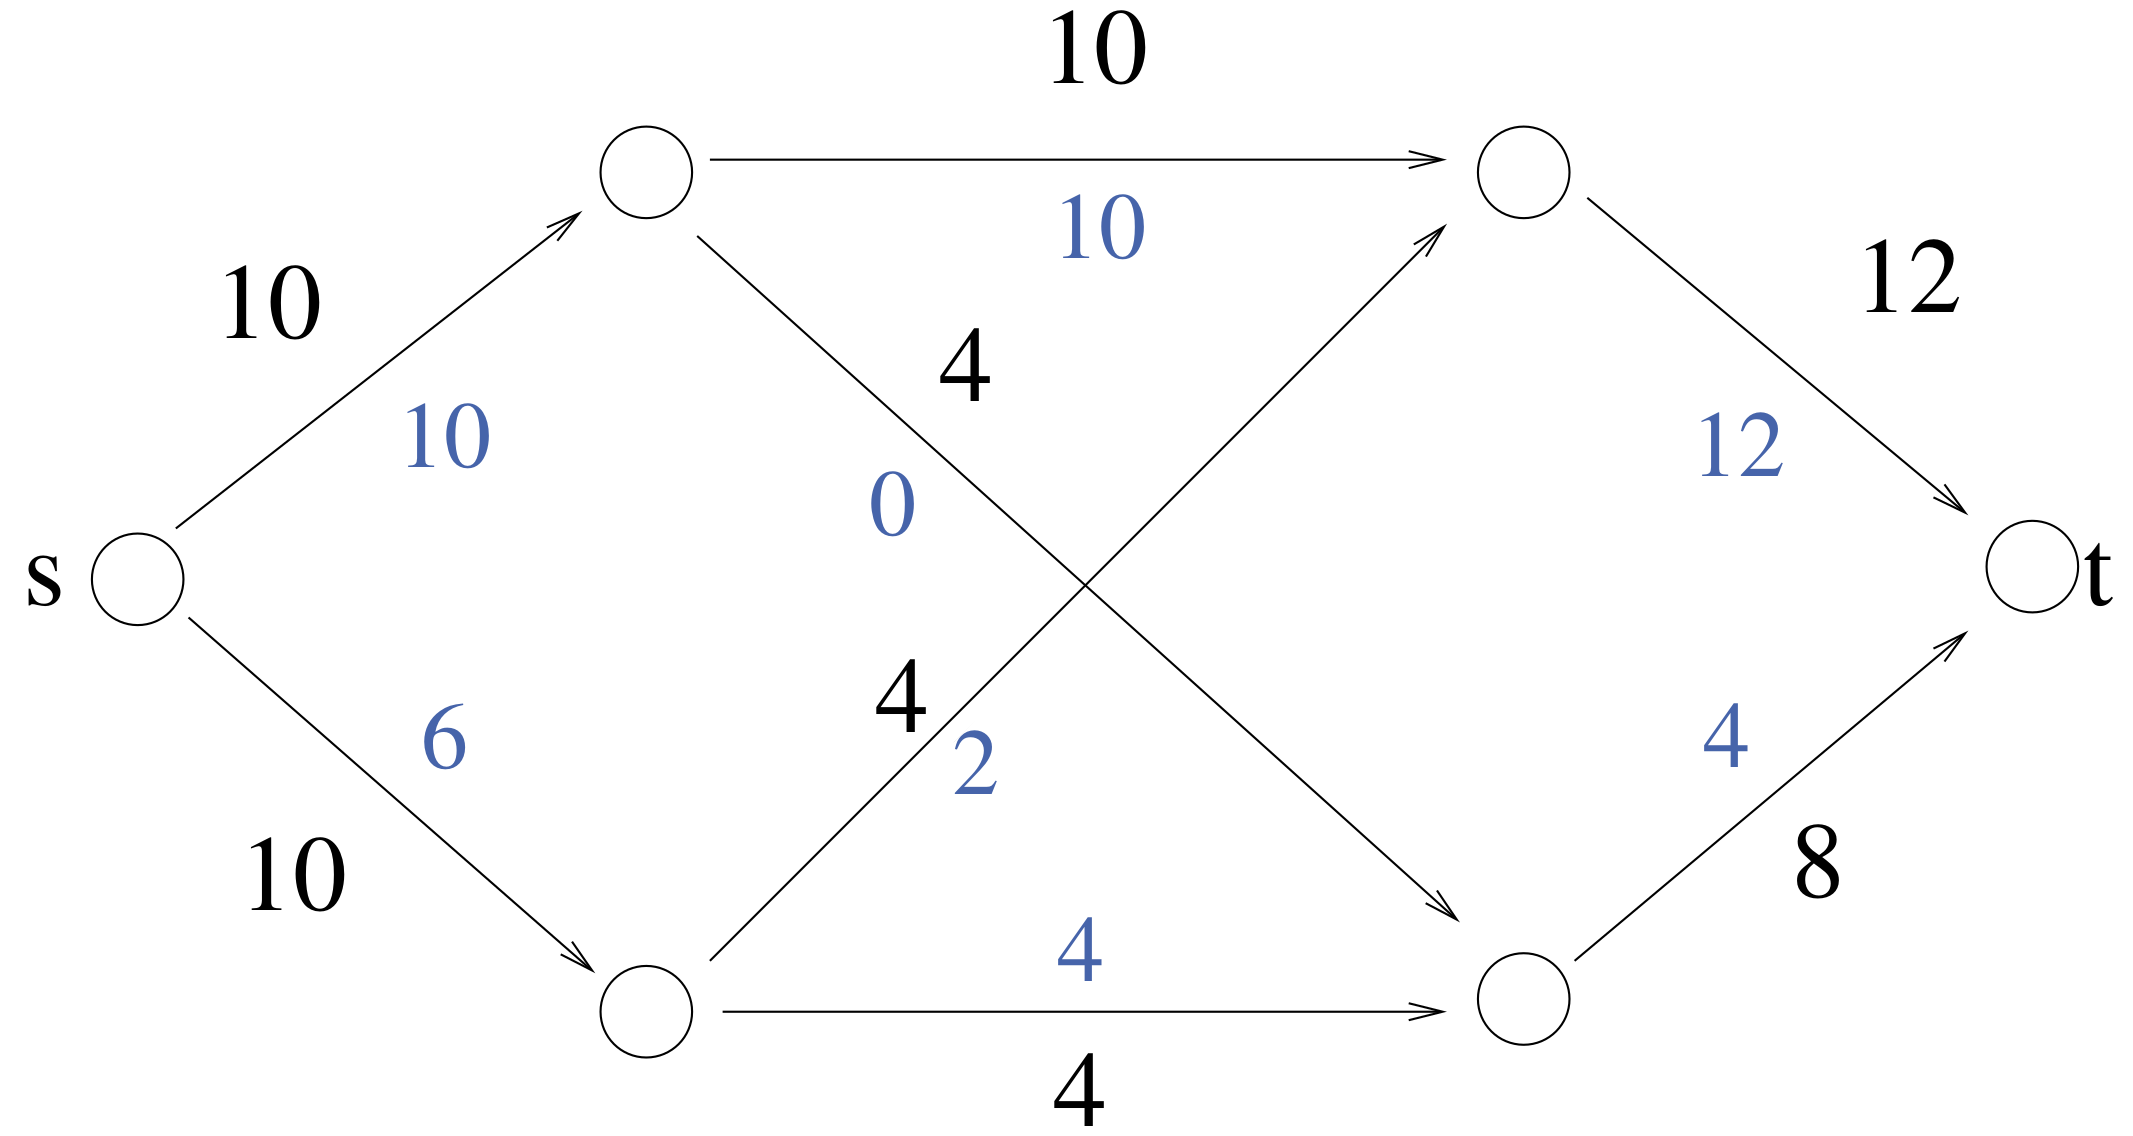
\includegraphics[width=\textwidth]{flow2}
    \caption{Nochmal der Fluss von oben}
  \end{figure}
\end{minipage}
\hfill
\begin{minipage}{.475\textwidth}
  \vspace{6.8mm}
  \begin{figure}[H]
    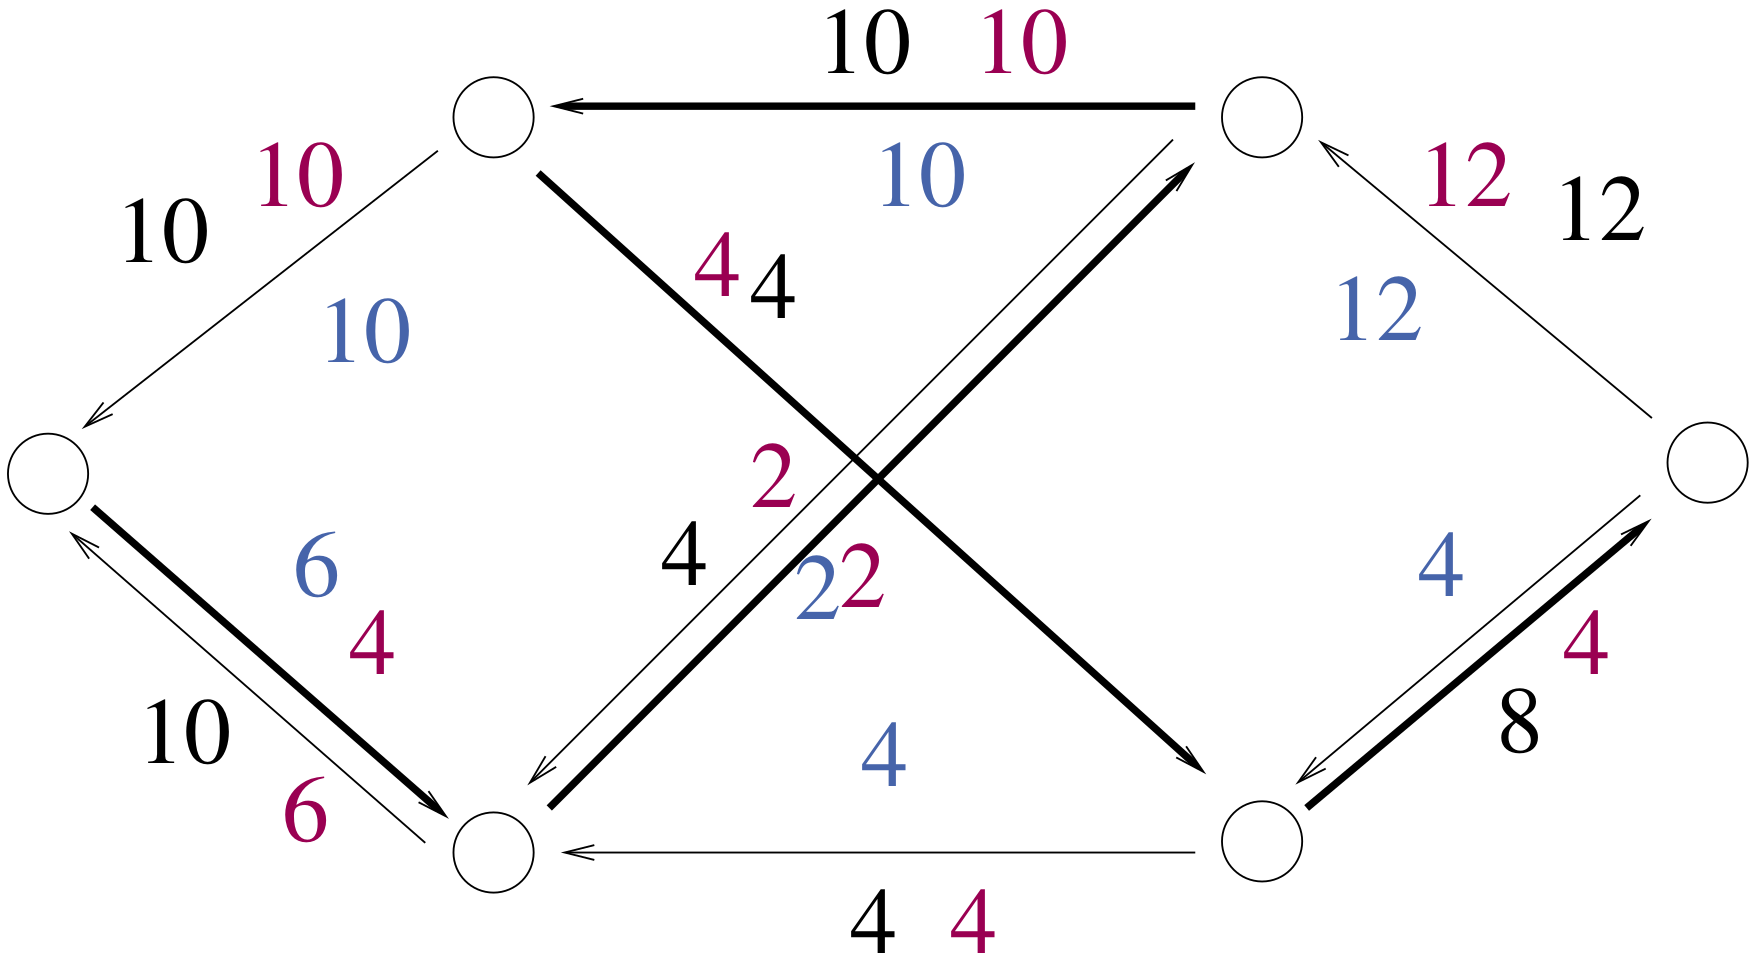
\includegraphics[width=\textwidth]{residualFlow}
    \caption{Der zu nebenstehendem Fluss gehörende Residualgraph. Schwarz die Kapazität, Blau der Fluss, Rot die residuale Kapazität}
  \end{figure}
\end{minipage}

Wir suchen jetzt nach einem \( s \)-\( t \)-Pfad \( p \), sodass jede Kante residuale Kapazität \( c_e^f \neq 0 \) hat:

\begin{pseudocode}
  \( \Delta f \coloneqq \min_{e \in p}c_e^f \) \\
  \textbf{foreach} \( (u,v) \in p \) \textbf{do} \\
  \phantom{\enskip} \textbf{if} \( (u,v) \in E \) \textbf{then} \( f_{(u,v)} \pluseq \Delta f \) \\
  \phantom{\enskip} \textbf{else} \( f{(v,u)} \minuseq \Delta f \)
\end{pseudocode}

Wir können nun den \term{Ford-Fulkerson-Algorithmus}\index{Ford-Fulkerson-Algorithmus} implementieren:

\begin{pseudocode}
  \textbf{\textsc{FFMaxFlow}}\( (G = (V,E), s, t, c: E \to \N) : E \to \N \) \\
  \phantom{\enskip} \( f \coloneqq 0 \) \\
  \phantom{\enskip} \textbf{while} \( \exists \) path \( p = (s,\dots,t) \) in \( G_f \) \textbf{do} \\
  \phantom{\enskip} \phantom{\enskip} augment \( f \) along \( p \) \\
  \phantom{\enskip} \textbf{return} f
\end{pseudocode}

Die Zeitkomplexität ist \( O(m*\text{val}(f)) \), da bei jedem Durchgang der Fluss um mindestens \( 1 \) erhöht wird und jedes Mal DFS \( O(m) \) ausgeführt werden muss.

\subsection{Problem --- Blocking Flows}

\begin{minipage}{.6\textwidth}
  Es gibt Netzwerke, in denen der Ford-Fulkerson-Algorithmus tatsächlich die längstmögliche Laufzeit braucht, obwohl die Lösung sehr trivial ist. Grund dafür sind sogenannte \term{Blocking Flows}\index{Fluss!Blocking Flow}.

  \( f_b \) ist ein \emph{blocking flow} in \( H \), falls für jeden \( s \)-\( t \)-Pfad \( p \) gilt:
  \begin{equation*}
    \exists \ e \in p : f_b(e) = c(e)\text{.}
  \end{equation*}
  Das bedeutet, dass jeder \( s \)-\( t \)-Pfad eine vollständig ausgelastete Kante beinhaltet.
\end{minipage}
\hfill
\begin{minipage}{.35\textwidth}
  \begin{figure}[H]
    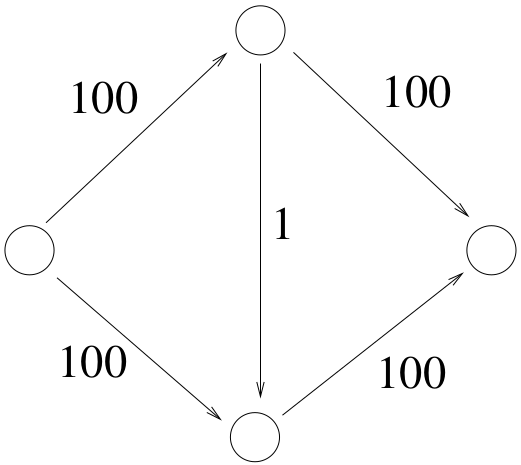
\includegraphics[width=\textwidth]{fulkersonBad}
    \caption{In diesem Netzwerk könnte der Ford-Fulkerson-Algorithmus stets einen Pfad über die mittlere Kante augmentieren und würde deswegen 200 Schritte brauchen}
  \end{figure}
\end{minipage}

\section{Dinic-Algorithmus}

Der \term{Dinic-Algorithmus}\index{Dinic-Algorithmus} sieht so aus:

\begin{pseudocode}
  \textbf{\textsc{DinitzMaxFlow}}\( (G = (V, E), s, t, c: E \to \N) : E \to \N \) \\
  \phantom{\enskip} \( f \coloneqq 0 \) \\
  \phantom{\enskip} \textbf{while} \( \exists \) path \( p = (s,\dots,t) \) in \( G_f \) \textbf{do} \\
  \phantom{\enskip} \phantom{\enskip} \( d = G_f\text{.\textcolor{red}{reverseBFS}}(t) : V \to \N \) \\
  \phantom{\enskip} \phantom{\enskip} \( \textcolor{red}{L_f} \coloneqq (V, \left \{ (u,v) \in E_f : d(v) = d(u) - 1 \right \}) \) \enskip{} \textcolor{gray}{// layer graph} \\
  \phantom{\enskip} \phantom{\enskip} \textcolor{red}{find blocking flow} \( f_b \) in \( L_f \) \\
  \phantom{\enskip} \phantom{\enskip} augment \( f \pluseq f_b \) \\
  \phantom{\enskip} \textbf{return} \( f \)
\end{pseudocode}

Die rot gekennzeichneten Funktionen/Objekte müssen wir noch klären.

Der Ablauf lässt sich folgendermaßen zusammenfassen:

\begin{enumerate}
  \item Berechne Distanz-Labels (Abstand zur Senke) für alle Knoten des Graphen.

   (Rückwärtsgerichtete Breitensuche von \( t \) aus)
  \item Stelle auf Basis der Distanz-Labels den Layer-Graph auf.
  \item Suche auf dem Layer-Graph einen blockierenden Fluss zwischen \( s \) und \( t \).
  \item Führe den gefundenen blockierenden Fluss auf dem Residualgraph aus und aktualisiere diesen entsprechend.
  \item Konstruiere den aktualisierten Layer-Graphen und gehe zu Schritt 3.
  \item Breche ab, sobald kein weiterer Fluss im Layer-Graph existiert.
\end{enumerate}

\subsection{Abstandsfunktion}

Die Abstandsfunktion \( d \) gibt den Abstand eines Knotens zur Senke \( t \) an.

\subsection{Layer-Graph}

Den \term{Layer-Graph}\index{Layer-Graph} eines Netzwerks erhält man, indem man alle Kanten aus dem Residualgraphen entfernt, die nicht von einer Schicht in die vorherige führen. Es werden also alle Kanten
\begin{itemize}
  \item innerhalb einer Schicht und
  \item zwischen Schicht \( i \) und \( i + k \) (\( k \in \N \))
\end{itemize}
entfernt. Formal ist das
\begin{equation*}
  L_f = (V, \left \{ (u,v) \in E_f : d(v) = d(u) - 1 \right \})\text{.}
\end{equation*}

Die Laufzeit des Dinic-Algorithmus ist damit in \( O(mn^2) \).
  \chapter{Externe Algorithmen}

\begin{minipage}{.6\textwidth}
  Greift man auf sehr große Datenbestände zu, so sind diese in der Regel auf Sekundärspeicher wie Platte oder Band gespeichert, weil diese sehr günstig sind. Problem ist, dass der Zugriff auf den Speicher sehr viel Zeit benötigt.
  
  \term{Externe Algorithmen}\index{Externe Algorithmen} nehmen an, dass die \emph{interne Arbeit}, also die Rechenarbeit, kostenlos ist. Minimiert werden soll die Anzahl an Zugriffen auf den Sekundärspeicher.
\end{minipage}
\hfill
\begin{minipage}{.35\textwidth}
  \begin{figure}[H]
    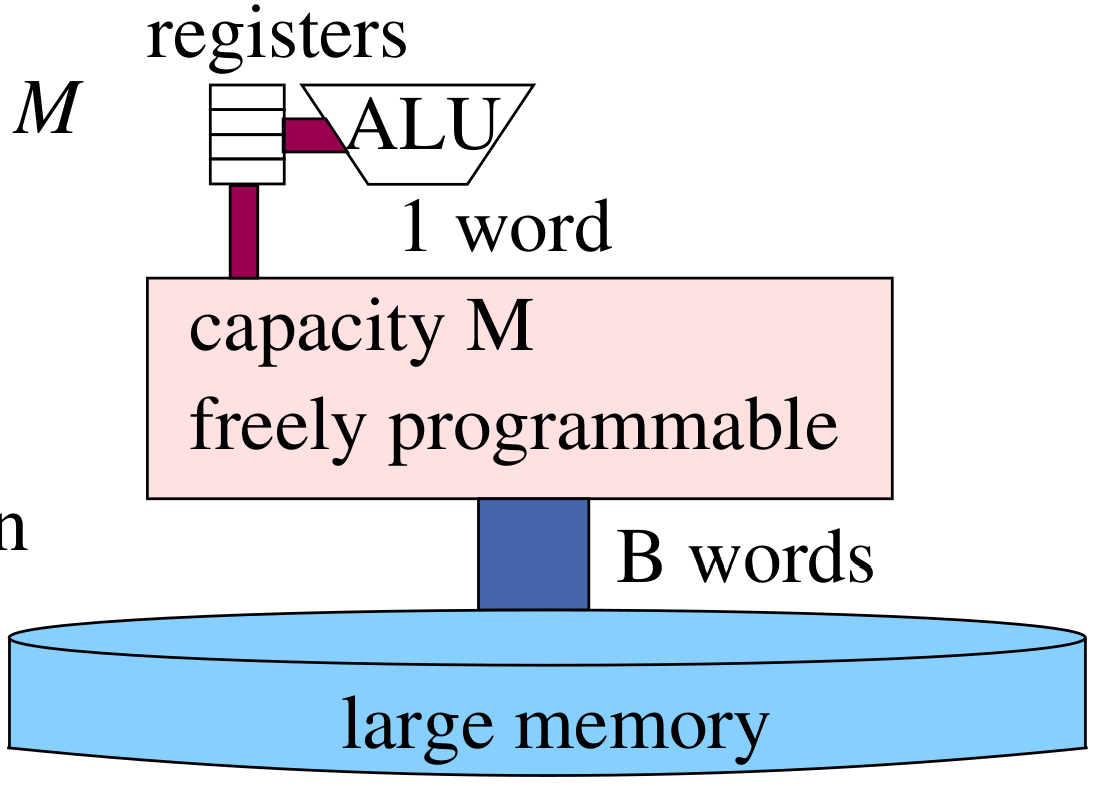
\includegraphics[width=\textwidth]{externalModel}
    \caption{Sekundärspeicher-modell mit schnellem internen Speicher der Größe \( M \) und einem beliebig großem externen Speicher, der über einen \( B \) Wörter breiten Bus angebunden ist}
  \end{figure}
\end{minipage}

\section{Mehrwegemischen}

Als nichttriviales Beispiel werden wir \term{Mehrwegemischen}\index{Mehrwegemischen} betrachten:

\begin{pseudocode}
  \textbf{\textsc{multiwayMerge}}\( (a_1,\dots,a_k,c : \text{File \textbf{of} Element}) \) \\
  \phantom{\enskip} \textbf{for} \( i \coloneqq 1 \) \textbf{to} \( k \) \textbf{do} \( x_i \coloneqq a_i\text{.readElement} \) \\
  \phantom{\enskip} \textbf{for} \( j \coloneqq 1 \) \textbf{to} \( \sum_{i=1}^k \left\vert a_i \right\vert \) \textbf{do} \\
  \phantom{\enskip} \phantom{\enskip} find \( i \in 1\dots k \) that minimizes \( x_i \) \enskip{} \textcolor{gray}{// no IOs, \( O(\log k) \) time} \\
  \phantom{\enskip} \phantom{\enskip} \( c\text{.writeElement}(x_i) \) \\
  \phantom{\enskip} \phantom{\enskip} \( x_i \coloneqq a_i\text{.readElement} \)
\end{pseudocode}

Der Aufwand beträgt

\begin{itemize}
  \item \textbf{I/O}: \( a_i \) lesen \( \approx \frac{\left\vert a_i \right\vert}{B} \), \( c \) schreiben \( \approx \sum_{i=1}^k \frac{\left\vert a_i \right\vert}{B} \)

  \( \Rightarrow \) Insgesamt \( \leq \approx 2\frac{\sum_{i=1}^k \left\vert a_i \right\vert}{B} \)

  \emph{Bedigungung}: brauchen \( k+1 \) Pufferblöcke.

  \item \textbf{Interne Arbeit} durch Benutzung einer Prioritätsliste:
  \begin{equation*}
    O\left( \log k \sum_{i=1}^k \left\vert a_i \right\vert \right)
  \end{equation*}
\end{itemize}

\subsection{Sortieren durch Mehrwegemischen}

Wir können Mehrwegemischen verwenden, um zu sortieren:

\begin{enumerate}
  \item Sortiere \( \left\lceil \tfrac{n}{M} \right\rceil \) runs mit je \( M \) Elementen.
  \item Mische jeweils \( \tfrac{M}{B} \) runs, bis nur noch ein run übrig ist.
\end{enumerate}

Die Anzahl an I/Os setzt sich aus \( 2\tfrac{n}{B} \) I/Os für das sortieren, \( 2\tfrac{n}{B} \) I/Os für das Mischen und \( \left\lceil \log_{M/B} \tfrac{n}{M} \right\rceil \) Mischphasen zusammen, insgesamt also

\begin{equation*}
  \text{sort}(n) \cong \frac{2n}{B}\left( 1 + \left\lceil \log_{M/B} \frac{n}{M} \right\rceil \right) \enskip \text{I/Os.}
\end{equation*}

Die interne Arbeit setzt sich zusmamen aus
\begin{itemize}
  \item run formation: \( O(n\log M) \),
  \item Zugriffe auf die Prioritätsliste pro Phase: \( O\left( n\log \tfrac{M}{B} \right) \),
  \item Anzahl Phasen: \( \left\lceil \log_{M/B} \tfrac{n}{M} \right\rceil \)
\end{itemize}
zusammen, insgesamt

\begin{equation*}
  O\left( n \log M + n\log \tfrac{M}{B} * \left\lceil \log_{M/B} \tfrac{n}{M} \right\rceil \right) = O(n\log n)\text{.}
\end{equation*}

  \printindex
  
\end{document}
